%You can delete all the comments after you have finished your document
%this sets up the defaults for the documents, 12pt font and A4 size. The article type sets this up as such as opposed to letter or memo.
%for the finer points LaTeX see https://en.wikibooks.org/wiki/LaTeX or http://tex.stackexchange.com/

\documentclass[12pt,a4paper]{article}
\usepackage{titlesec} %these are how we import packages, one helps set up footers and title layout
\usepackage{fancyhdr}

% !TEX TS-program = pdflatex
% !TEX encoding = UTF-8 Unicode
\usepackage[utf8]{inputenc} % set input encoding (not needed with XeLaTeX)
%\usepackage[margin=3.5cm]{geometry}

\usepackage{graphicx} % support the \includegraphics command and options

% \usepackage[parfill]{parskip} % Activate to begin paragraphs with an empty line rather than an indent

%%% PACKAGES
\usepackage{booktabs} % for much better looking tables
\usepackage{array} % for better arrays (eg matrices) in maths
\usepackage{paralist} % very flexible & customisable lists (eg. enumerate/itemize, etc.)
\usepackage{verbatim} % adds environment for commenting out blocks of text & for better verbatim
\usepackage{subfig} % make it possible to include more than one captioned figure/table in a single float
\usepackage[british]{babel}
\usepackage[style=apa,backend=biber]{biblatex}
\DeclareLanguageMapping{british}{british-apa}
\usepackage[toc,page]{appendix}
% These packages are all incorporated in the memoir class to one degree or another...

\usepackage{tikz}
\usetikzlibrary{matrix,chains,positioning,decorations.pathreplacing,arrows}

% MY PACKAGES
%\usepackage[table]{xcolor}
\usepackage{color, colortbl}
\usepackage{amsmath}
\usepackage{adjustbox}
\usepackage{pdfpages}
\usepackage{pgfplots}
\usepackage{multicol}
\usepackage{float}
\usepackage{blindtext}
\usepackage{longtable}
\usepackage{subcaption}
\usepackage{xr}

% EXTERNAL DOCUMENTS
\externaldocument{figures/kfoldfigure}
\externaldocument{figures/onehot}
\externaldocument{tables/kddattacks}
\externaldocument{tables/classifierconfig}


\makeatletter
\renewcommand\paragraph{\@startsection{paragraph}{4}{\z@}%
  {-2.5ex\@plus -1ex \@minus -.25ex}%
  {1.25ex \@plus .25ex}%
  {\normalfont\normalsize\bfseries}}
\makeatother

\setcounter{secnumdepth}{4} % how many sectioning levels to assign numbers to
\setcounter{tocdepth}{4} % how many sectioning levels to show in ToC


%header and footer settings
\pagestyle{fancyplain}
\fancyhf{}
\renewcommand{\headrulewidth}{0.5pt}
\renewcommand{\footrulewidth}{0.5pt}
\setlength{\headheight}{15pt}
\fancyhead[L]{Jack Anderson - 40208539}
\fancyhead[R]{ SOC10101 Honours Project}
\fancyfoot[L]{}
\fancyfoot[C]{\thepage}

%set better section layout
\makeatletter
\renewcommand\subsection{\@startsection {subsection}{1}{2mm} % name, level, indent
      {3pt plus 2pt minus 1pt} % before skip
      {3pt plus 0pt} % after skip
      {\normalfont\bfseries}}
\makeatother
\makeatletter
\renewcommand\section{\@startsection {section}{1}{0mm} % name, level, indent
      {4pt plus 2pt minus 1pt} % before skip
      {4pt plus 0pt} % after skip
      {\bfseries}}
\makeatother

\addbibresource{bibliography.bib}

%this starts the document
\begin{document}

%you can import other documents into your main one, these layout the Title and Declarations on its own page.
%you might need to change these to \ if your on Microsoft Windows.
\newcommand{\HRule}{\rule{\linewidth}{0.5mm}}

\begin{titlepage}
	\begin{center}

	\HRule \\[0.4cm]
    	{\Large \bfseries A Comparison Of Machine Learning Algorithms to Detect Network Intrusions\par}
	\vspace{0.2cm}
	\HRule \\[1.5cm]

	
    	\vspace{3cm}
	\begin{minipage}{0.4\textwidth}
	\begin{center} \large
        \emph{}\\
        	Jack Anderson - 40208539
				
   	 \end{center}
    	\end{minipage}
	
	\vspace{2cm}
    	\begin{minipage}{1\textwidth}
    	\begin{center} \large
        
		Submitted in partial fulfilment of \\
		the requirements of Edinburgh Napier University \\
		for the Degree of \\
        	BEng (Hons) Software Engineering
    	\end{center}
    	\end{minipage}

    	\vfill

    	% Bottom of the page
	\begin{minipage}{1\textwidth}
    	\begin{center} \large
		School of Computing
    	\end{center}
    	\end{minipage}
	
	\vspace{1cm}
    	{\large \today}


	\end{center}
\end{titlepage}
%{\large Submitted in partial fulfilment of the requirements of Edinburgh Napier University for the Degree of }

\section*{Authorship Declaration}
\vspace{0.5cm}
\begin{flushleft}
I, (Insert Name eg. Norman Stanley Fletcher), confirm that this dissertation and the work presented in it are my own achievement.\newline

Where I have consulted the published work of others this is always clearly attributed;\newline

Where I have quoted from the work of others the source is always given. With the exception of such quotations this dissertation is entirely my own work;\newline

I have acknowledged all main sources of help; \newline

If my research follows on from previous work or is part of a larger collaborative research project I have made clear exactly what was done by others and what I have contributed myself;\newline

I have read and understand the penalties associated with Academic Misconduct.\newline

I also confirm that I have obtained informed consent from all people I have involved in the work in this dissertation following the School's ethical guidelines.\newline
\end{flushleft}

\begin{flushleft} \large
\emph{Signed:} \\
\end{flushleft}

\vspace{.5cm}

\begin{flushleft} \large
\emph{Date:} \\
\end{flushleft}

\vspace{.5cm}

\begin{flushleft} \large
\emph{Matriculation no: }  \\
\end{flushleft}
\pagebreak

\section*{Data Protection Declaration}
\vspace{0.5cm}
\begin{flushleft}
Under the 1998 Data Protection Act, The University cannot disclose your grade to an unauthorised person. However, other students benefit from studying dissertations that have their grades attached. \newline

\vspace{0.5cm}

Please sign your name below one of the options below to state your preference.\newline
\vspace{0.5cm}

The University may make this dissertation, with indicative grade, available to others.\newline
\vspace{1cm}
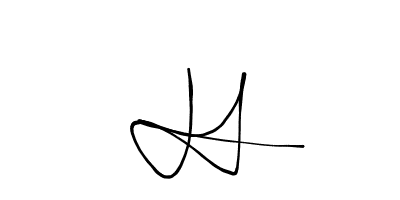
\includegraphics[width=0.4\textwidth, center]{figures/signature}

The University may make this dissertation available to others, but the grade may not be disclosed.\newline
\vspace{3cm}


The University may not make this dissertation available to others.\newline
\end{flushleft}


\pagebreak

%LaTeX let you define the abstract separately so it wont get sucked into the main document.
\begin{abstract}
% fill the abstract in here
\end{abstract}
\pagebreak

\tableofcontents % is generated for you
\newpage

\listoftables
%generated in same way as figures
\newpage

\listoffigures
%you may have captions such as equations, listings etc they should all appear as required
%these are done for you as long as you use \begin{figure}[placement settings] .. bla bla ... \end{figure}
\newpage

\section*{Acknowledgements}
Insert acknowledgements here
\newpage

\section{Introduction}
\subsection{Background}
	For any major company or business security is of the utmost concern, with a study finding that in the UK in 2016 an estimated 46\% of all businesses experienced a cyber security breach or attack \cite{securitysurvey2017}. These breaches are particularly dangerous as even if a network is compromised a single time a company can have its entire database destroyed, or customer data leaked, leading to legal repercussions. When it comes to preventing these intrusions firewalls alone are insufficient for anything but the most rudimentary of attacks and so a Network Intrusion Detection System (NIDS) is employed to further bolster the security of the network. Traditional NIDS are placed strategically on a network to monitor all incoming traffic. It analyses the passing traffic and then compares it to a large library of known attacks and if it matches will flag the traffic. While these systems do provide some degree of protection they are unable to detect novel attacks or zero-day vulnerabilities and so some other method of identifying suspicious traffic is required. Introducing machine learning to a NIDS is one way of attempting to solve this problem first proposed by \cite{denning1987intrusion}. In using machine learning to detect network intrusions the system can be trained to recognise patterns of intrusive behaviour, allowing it to detect attacks which it may not have seen before but have characteristics of similar attacks. Machine learning also allows systems to be easily retrained to accommodate for new data on attacks as it emerges. There are two main categories of NIDS: misuse detection, and anomaly detection; both of which have their own advantages and disadvantages. This literary review aims to discuss the different kinds of network intrusion detection systems, the algorithms that these systems employ, and the gap in papers which directly compare the performance of single stage and two-stage classifiers in the domain of network intrusion detection.
		
\subsection{Research Questions}
	For this honours thesis there are a number of research questions which have been collated, and an attempt made to answer them. These questions in which I am interested in answering are the following: 
		
		\begin{itemize}
			\item What is the rate of accurate detection and classification of network intrusions by single stage machine learning classification methods?
			\item What is the rate of accurate detection and classification of network intrusions by two stage machine learning classification methods?
			\item Which method of classification i.e. single stage or two stage, is more accurate and by what amount?
			\item Which configuration of algorithms in the two stage classifier produces the most accurate results?
		\end{itemize}
		
In this context, accuracy is defined as a high number of true positives and true negatives, and a low number of false positives and false negatives when classifying network intrusions. \\

	First research will be completed in order to gain an understanding of the history and current state of machine learning for network intrusion detection, through reading relevant research papers and articles. Next the individual algorithms and methods which go into detecting network intrusions will be researched and understood. This knowledge will then be put into developing a piece of software capable of running these algorithms and extracting metrics which will be used to answer these research questions.

\subsection{Aims and Objectives}
	The aim of this project is to create a piece of software which is capable of running both single and two stage classification algorithm arrangements on a number of datasets and displaying the results in a clear manner. In doing so this will assist in answering the research questions put forward.

	These research questions, specifically whether or not two stage classification provides more accurate results than single stage classification will be answered by meeting the following objectives:
\begin{itemize}
\item{Perform a review of existing literature.}
\item{Perform a review of existing software.}
\item{Select appropriate machine learning classification algorithms.}
\item{Select appropriate datasets for use in network intrusion detection.}
\item{Implementation of software to assist in comparison of classification algorithms.}
\item{Evaluation of software with regards to specification and other software.}
\item{Evaluation of classification algorithm performance.}
\end{itemize}

\subsection{Scope and Limitations}
	\subsubsection{Deliverables}
	The list of deliverables for this project are the following:
	\begin{itemize}
	\item{A review of literature on related topics and a report detailing the findings of such reports.}
	\item{A review of existing software which performs a similar role to the proposed software.}
	\item{A software requirement specification.}
	\item{A description of all testing which will be carried out.}
	\item{A report detailing the results of each classification algorithm and configuration of two stage classification algorithms}
	\item{An evaluation of the implemented software with regards to how well it meets the proposed specification, and how it compares to existing software.}
	\end{itemize}
	\subsubsection{Boundaries}
	There exists a large number of different classification algorithms and methods to perform network intrusion detection, therefore this project must focus on a few specifically. This project will focus on performing misuse detection rather than anomaly detection, and will limit the classification algorithms used to: k-Nearest Neighbour, Multi-layer Perceptron, and a Support Vector Machine.
	\subsubsection{Constraints}
	The largest constraint facing this project is that of time. There is a large amount of literature to be reviewed, and also a considerable amount of results which must be collected and results drawn from in a short amount of time.
	Time
	Knowledge
	Misuse detection only
\subsection{Structure of this Dissertation}
This dissertation can be divided into three main parts. Part one is literature review and past projects within the field, and existing software. Second part details the planning design and implementation of the software and the third consists of an analysis and evaluation of results and software.

part one reviews the literature on the subject and examines results of past projects and individual algorithms, also reviews existing software for machine learning comparison.

part two describes the detailed software requirements and specific functionality which should be implemented. Also includes a description of technologies and libraries used, and a testing plan. 

part three is an evaluation of the final software product against its design. Analysis and evaluation of classifier results. also has an evaluation of the overall project how well it met its aims and suggestions for future work.

\section{Literature Review}

	\subsection{Introduction}
		For any major company or business security is of the utmost concern, with a study finding that in the UK in 2016 an estimated 46\% of all businesses experienced a cyber security breach or attack \cite{securitysurvey2017}. These breaches are particularly dangerous as even if a network is compromised a single time a company can have its entire database destroyed, or customer data leaked, leading to legal repercussions. When it comes to preventing these intrusions firewalls alone are insufficient for anything but the most rudimentary of attacks and so a Network Intrusion Detection System (NIDS) is employed to further bolster the security of the network. Traditional NIDS are placed strategically on a network to monitor all incoming traffic. It analyses the passing traffic and then compares it to a large library of known attacks and if it matches will flag the traffic. While these systems do provide some degree of protection they are unable to detect novel attacks or zero-day vulnerabilities and so some other method of identifying suspicious traffic is required. Introducing machine learning to a NIDS is one way of attempting to solve this problem first proposed by \cite{denning1987intrusion}. In using machine learning to detect network intrusions the system can be trained to recognise patterns of intrusive behaviour, allowing it to detect attacks which it may not have seen before but have characteristics of similar attacks. Machine learning also allows systems to be easily retrained to accommodate for new data on attacks as it emerges. There are two main categories of NIDS: misuse detection, and anomaly detection; both of which have their own advantages and disadvantages. This literary review aims to discuss the different kinds of network intrusion detection systems, the algorithms that these systems employ, and the gap in papers which directly compare the performance of single stage and two-stage classifiers in the domain of network intrusion detection.
		
	\subsection{Research Questions}
		For this honours thesis there are a number of research questions which have been collated, and an attempt made to answer them. These questions in which I am interested in answering are the following: 
		
		\begin{itemize}
			\item What is the rate of accurate detection and classification of network intrusions by single stage machine learning classification methods?
			\item What is the rate of accurate detection and classification of network intrusions by two stage machine learning classification methods?
			\item Which method of classification i.e. single stage or two stage, is more accurate and by what amount?
			\item Which configuration of algorithms in the two stage classifier produces the most accurate results?
		\end{itemize}
		
In this context, accuracy is defined as a high number of true positives and true negatives, and a low number of false positives and false negatives when classifying network intrusions. \\

		First research will be completed in order to gain an understanding of the history and current state of machine learning for network intrusion detection, through reading relevant research papers and articles. Next the individual algorithms and methods which go into detecting network intrusions will be researched and understood. This knowledge will then be put into developing a piece of software capable of running these algorithms and extracting metrics which will be used to answer these research questions.
	\subsection{Search Strategy}
While searching for relevant papers on the subject of network intrusion detection, a number of key terms were identified which could be used to find papers within the field. The main search term which was used was \textit{'Network Intrusion Detection'} which was used to find papers which were generally related to the topic. A number of suplemental search terms were identified and used in conjuntion with the main search term when attempting to find papers which used a specific technology within network intrusion detection. These included: 'Nearest Neighbor', 'k-NN', 'Neural', 'Self Organising Map', 'SOM', 'Recurrent', 'Hybrid', 'Stage', and 'Ensemble'. Using a combination of the main search term and these additions search terms allowed the discovery of papers directly relevant to the project. If two terms were required to be included within the search then the \textbf{AND} operator would be used to ensure that both were matched. Similarly if there were multiple terms for the same technique or technology, i.e. 'Nearest Neighbor' and 'k-NN' then the \textbf{OR} operator would be used, to reduce the number of individual searches which were required to be carried out. When papers were found and deemed relevant to the project, a review of citations included within those papers would also be carried out, which allows the finding of papers which are directly related to the subject but which may have been missed by the search terms specified. A seperate search was also performed when researching a relevant dataset by searching for the title of each dataset, such as: 'KDD Cup', 'NSL-KDD', 'DARPA', etc. 

	\subsection{Databases}
		To find appropriate research papers, Google Scholar and the Edinburgh Napier University Library Search were used to locate articles and other databases which could also be searched. The databases from which the papers were retrieved were:
		\begin{itemize}
			\item ScienceDirect
			\item IEEE Xplore
			\item ACM Digital Library
			\item Society for Industrial and Applied Mathematics
		\end{itemize}
		
	\subsection{Paper Selection}
	At first a large range of papers were collected by title and held on to that could be relevant to the subject matter. Then the abstract and conclusion were read through to determine whether or not the paper was relevant to the research questions. Once the pool of papers had been reduced to a manageable size the entire paper was read through to attempt to make links between the content of the paper and the work which would be carried out and how they could assist in answering the research questions. 

	\vspace{5mm}

	\noindent During this process, papers would be selected for use if they met all of the following criteria:
	\begin{itemize}
	\item Peer reviewed.
	\item If the paper is older than five years and has at least 50 citations.
	\item The paper is directly relevant to the research questions.
	\end{itemize} 
		
	\vspace{5mm}
	
	\noindent Papers would be rejected if they met any of the following critera:
	\begin{itemize}
	\item Too broad.
	\item Cannot be directly applied to the research questions.
	\item The paper has less than fifty citations and is older than five years.
	\item A newer more relevant paper on topic was found.
	\end{itemize}
	
	\subsection{Network Intrusion Detection}
	The field of network intrusion detection was conceived by \cite{denning1987intrusion}, a paper in which the author describes a model for a "real-time intrusion-detection expert system" capable of discerning between normal and abnormal network activity.
	NIDS can be broadly categorized as performing either: misuse detection or anomaly detection. 
	Misuse detection systems are first trained using some kind of learning algorithm on a set of labelled data where each entry is defined as being either 'normal' or 'intrusive'. Using this the system can create a sophisticated model of attacks, with a very high accuracy in detecting previously observed attacks and variations of such attacks. However, these types of systems perform poorly when faced with novel attacks being unable to accurately detect and classify them.
	
	Anomaly detections systems are trained on a set of data in which every entry is an example of 'normal' network traffic. Training the system in such a way means that \textit{"behavior is flagged as a potential intrusion if it deviates significantly from expected behavior"}\cite{Javitz1994TheNS}. This allows such systems to easily detect novel attacks which have not been observed before. Although these systems perform well at detecting novel attacks they also have a much higher false positive rate than misuse detection systems. The reason for this is that \textit{"previously  unseen  (yet  legitimate)  system  behaviors are also recognized as anomalies, and hence flagged as potential intrusions"} \cite{lazarevic2003comparative}. Anomaly detection systems also suffer from a so called \textit{"semantic gap"} where anomalies can be detected yet there is no further information on what type of attack has been performed \cite{sommer2010outside}.
	
	In the beginning of network intrusion detection research methods were proposed for an expert system NIDS \cite{Ilgun1995rule}, in which took knowledge from experts within the network security field and encoded them into rules with which the system could use to check traffic with to determine if it was intrusive. Then in \cite{Lee1999framework} a framework was proposed for the use of data mining for building NIDS. This was the first to employ machine learning in its approach to detecting intrusions, a method which today has been explored extensively. In using this approach to network intrusion detection the NIDS can detect attacks which have not been seen before, and can also be retrained quickly on data of new which have appeared, whereas an expert system would need updated in an expensive and slow process.
	
	More recently hybrid approaches to network intrusion detection have been proposed in papers such as; \cite{powers2008hybrid} and, \cite{panda2012hybrid}, which employ a two stage classification approach. This two stage classification functions by first classifying network traffic as either 'normal' or 'intrusive'. Once intrusive traffic has been identified it is fed into a second stage which then determines the type of intrusion. Performing the detection and classification in this manner is beneficial as two separate classifiers can be used, allowing each to specialise, producing a higher rate of intrusion detection and a lower false positive rate.
	
	The research questions which this dissertation aims to answer are surrounding the comparison of these hybrid approaches in comparison to single stage monolithic detectors, which is discussed in more detail in section \ref{Research Contribution}. 
	
	\subsection{Machine Learning Algorithms}
	This section will detail the Machine learning algorithms which have been chosen to be evaluated and compared in this thesis.
	\subsubsection{k-Nearest Neighbours}
	The k-nearest neighbours (k-NN) is one of the most simple machine learning classification and regression algorithms. k-NN is a lazy algorithm meaning that it uses the training dataset directly and therefore does not require any training time. The algorithm functions by first taking a training set of labelled vectors. A vector which is to be classified is then input, and the algorithm calculates the distance from the input vector to each other point in the training set and selects the k nearest points from the training set. For each of these k nearest points their classifications are totalled and the classification which makes up the most of these neighbours is then output as the class of the input vector.
	In both \cite{liao2002use}, and in \cite{hautamaki2004outlier}, it has been demonstrated that k-NN based network intrusion detection methods can produce good results. The k-NN algorithm has been selected for this thesis mainly because of its simplicity and according to \cite{jain2000statistical} it \textit{"can  be  conveniently  used  as  a benchmark  for  all  the  other  classifiers  since  it  appears  to always  provide  a  reasonable  classification  performance  inmost applications."}.
	
	\subsubsection{Artificial Neural Network}
	According to \cite{caudill1987neural} an artificial neural network (ANN) is \textit{"a computing system made up of a number of simple, highly interconnected processing elements, which process information by their dynamic state response to external inputs"}. The ANN is inspired by and aims to recreate the operation of a biological neural network, found within the brains of living animals. The neural network consists of several layers of neurons or nodes, which are interconnected by axioms each of which has its own associated weight which is altered over the course of the training of the network. These weights are adjusted through a method called backpropagation. A network will typically consist of three layers; the input layer, the hidden layer(s), and the output layer, shown in Figure \ref{fig:ANN}.
	
	\begin{figure}[h]
\centering
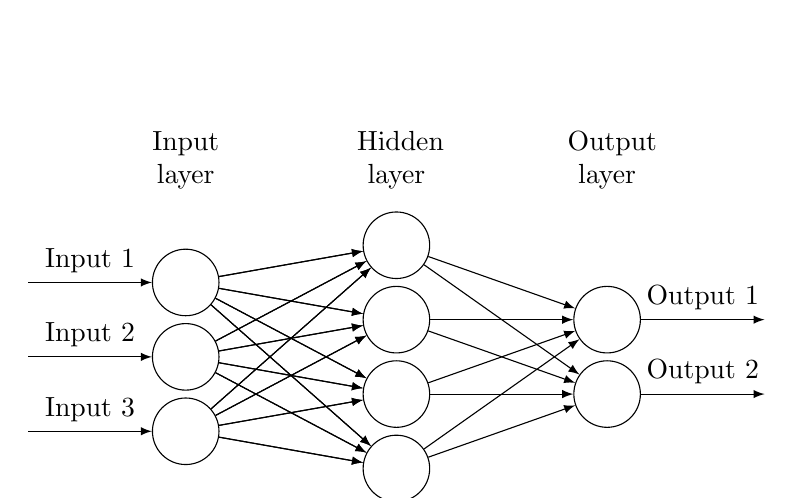
\begin{tikzpicture}[
plain/.style={
    draw=none,
    fill=none,
},
net/.style={
    matrix of nodes,
    nodes={
        draw,
        circle,
        inner sep=8.5pt
    },
    nodes in empty cells,
    column sep=0.6cm,
    row sep=-11pt
},
>=latex
]

\matrix[net] (mat)
{
    |[plain]| \parbox{1cm}{\centering Input\\layer} & |[plain]| \parbox{1cm}{\centering Hidden\\layer} & |[plain]| \parbox{1cm}{\centering Output\\layer} \\
    |[plain]| & \\
    & |[plain]| \\
    |[plain]| & &  \\
    & |[plain]| \\
    |[plain]| & &  \\
    & |[plain]| \\
    |[plain]| & \\
};
\foreach \ai [count=\mi ]in {3,5,7}
\draw[<-] (mat-\ai-1) -- node[above] {Input \mi} +(-2cm,0);
\foreach \ai in {3,5,7}
{\foreach \aii in {2,4,...,8}
    \draw[->] (mat-\ai-1) -- (mat-\aii-2);
}
\foreach \ai in {2,4,...,8}
\draw[->] (mat-\ai-2) -- (mat-6-3);

\foreach \ai in {2,4,...,8}
\draw[->] (mat-\ai-2) -- (mat-4-3);

\foreach \ai [count=\mi ]in {4,6}
\draw[->] (mat-\ai-3) -- node[above] {Output \mi} +(2cm,0);
\foreach \ai in {3,5,7}
{\foreach \aii in {2,4,...,8}
    \draw[->] (mat-\ai-1) -- (mat-\aii-2);
}
\end{tikzpicture}
\caption{Artificial Neural Network Layers}
\label{fig:ANN}
\end{figure}
	
	The input layer is where the neural network receives the data which it is to process. This input layer is then connected via weighted axioms to the hidden layer(s). The hidden layer may consist of many layers and is responsible for the recognition of patterns within the input data. These hidden layers are then connected to the output layer, which gives the result or classification of the input data.
	The ANN is trained by feeding in a labelled dataset containing inputs and expected output(s). Each data entry which is fed into the network slightly alters the weights of all axioms within the network depending on the inputs and outputs, which when performed a large number of times allows the network to recognise patterns within input data and attempt to predict the correct output.
	Neural networks were first proposed for use within the field of network detection intrusion by \cite{debar1992neural}, who found them to be a promising method. ANNs are especially good for use with data classification problems and in turn with network intrusion detection as they can recognise complex patterns within datasets with a large number of features, such as network traffic \cite{sung1998ranking}. Some early methods of network intrusion detection were also unable to make any sort of classification beyond a binary one, i.e. normal or intrusive, whereas ANNs can classify data into any number of categories allowing for a greater amount of information about an attack to be gained from the detection \cite{moradi2004neural}.
	
	However, while neural networks excel at classifying information and recognising complex patterns within data, they do suffer from a semantic gap. \cite{garcia2009anomaly} explain that \textit{"they do not provide a descriptive model that explains why a particular detection decision has been taken."} meaning that the network is essentially a black box, and without the details of the operation of the network it is difficult to determine what features of a connection identify it as intrusive and how effectively it may perform on other tasks and in other areas. The remainder of this section will discuss several different kinds of ANN which have been successfully applied to network detection intrusion.

This basic form of neural network is also called a feed forward neural network (FFNN) and is the most simple class of neural network available in which the connections between neurons do not form a cycle unlike in a RNN, i.e. information only travels forward from input neurons to output neurons.
	These kinds of neural networks have been employed in a number of research papers to great effect. \cite{mukkamala2002intrusion} found that with the use of a neural network intrusions could be accurately detected more than 99\% of the time. The same result was also found in \cite{zhang2001hide} with a 99\% detection rate.
\cite{linda2009neural}, \cite{lee2001training}, and \cite{moradi2004neural} also all achieved the same results as other studies. Using these results it is clear that using a FFNN is a viable method detecting network intrusions, as well as being simple to implement within a limit time frame. \cite{lee2001training} also found that these networks are extremely adept at detecting novel attacks which is a desirable trait in a NIDS. It is for these reasons that a FFNN has been chosen to be implemented in this thesis.

	\subsubsection{Self Organising Map}
	The self organising map (SOM) is a type of ANN first proposed in the paper \cite{kohonen1982self} and is used to map high dimensional data into lower dimensions. The SOM is unlike the other neural networks which are to be examined as it can learn to classify data without supervision. This means that whereas a regular neural network will require an input vector and and output vector, the SOM will learn to classify data without the need for an output vector. This lack of need for supervised training can be extremely useful in the context of network intrusion detection as described by \cite{rhodes2000multiple} \textit{"This approach is particularly powerful because the self-organizing map never needs to be told what intrusive behaviour looks like.  By learning to characterize normal behaviour, it implicitly prepares itself to detect any aberrant network activity."} both in anomaly detection and especially in misuse detection as normal behaviour can be continuously fed into it without the need for examples of intrusive behaviour.
	
	The SOM has been implemented and tested within a number of research papers with great success. In \cite{powers2008hybrid} and \cite{depren2005intelligent} it was found that the use of an SOM showed favourable false positive rates and attack classification results over other intrusion detection methods using the KDD 1999 Cup dataset. Similarly, in \cite{lichodzijewski2002dynamic} the researchers found that a SOM produced good results on the DARPA 1998 dataset with a low false positive rate and a correct classification rate of more than 95\%. \cite{kayacik2003som} too found SOM to be an effective method of classification with results much similar to the previous studies performed on the KDD 1999 Cup dataset however with a much higher rate of false positives.
	
	These papers demonstrate that the SOM is a viable method for the detection of network intrusions giving high rate of correct classifications and low false positive rate, however this algorithm will not be implemented as part of this thesis. This algorithm has been chosen to not be implemented due to an unfamiliarity on the part of the researcher and also time constraints of the project associated with this unfamiliarity regarding the research and implementation it, with other methods being less time consuming to implement.
	
	\subsubsection{Recurrent Neural Network}
	A recurrent neural network (RNN) is a class of artificial neural network where the connections within the network connect back to previous neurons in order to form a cycle of nodes as shown in Figure \ref{fig:RNN}. Having the neural network be structured in this manner allows it to process a sequence of input vectors allowing it to process data which relies on other vectors for context. RNNs are typically applied to problems such as handwriting recognition or speech recognition, however they can be particularly effective in network detection intrusion in recognising sequences of network traffic which alone are not suspicious but in a specific order can then be classified as intrusive behaviour.

		\tikzset{%
  every neuron/.style={
    circle,
    draw,
    minimum size=1cm
  },
  neuron missing/.style={
    draw=none, 
    scale=4,
    text height=0.333cm,
    execute at begin node=\color{black}$\vdots$
  },
}

    \def\layersep{2.5cm}

\begin{figure}[h]
\begin{center}
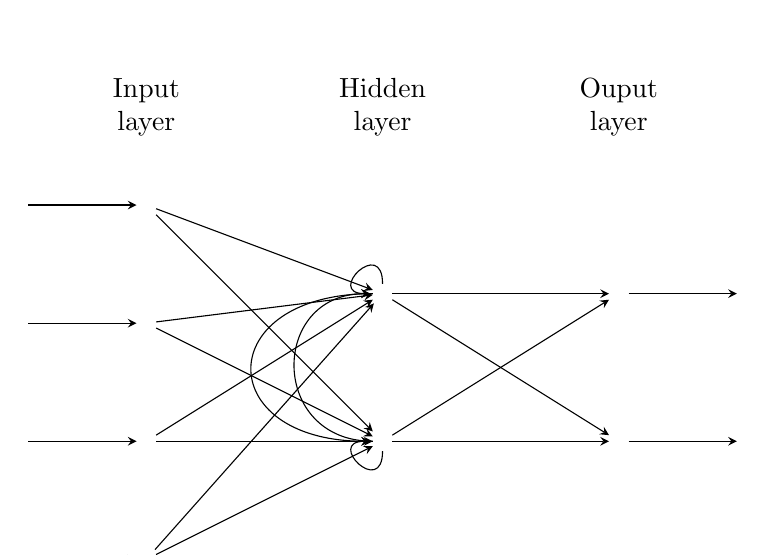
\begin{tikzpicture}[x=1.5cm, y=1.5cm, >=stealth]

\foreach \m/\l [count=\y] in {1,2,3,4}
  \node [every neuron/.try, neuron \m/.try] (input-\m) at (0,2.5-\y) {};

\foreach \m [count=\y] in {1,2}
  \node [every neuron/.try, neuron \m/.try ] (hidden-\m) at (2,2-\y*1.25) {};

\foreach \m [count=\y] in {1,2}
  \node [every neuron/.try, neuron \m/.try ] (output-\m) at (4,2-\y*1.25) {};

\foreach \l [count=\i] in {1,2,3,n}
  \draw [<-] (input-\i) -- ++(-1,0)
    node [above, midway] {};

\foreach \l [count=\i] in {1,n}
  \node [above] at (hidden-\i.north) {};

\foreach \l [count=\i] in {1,n}
  \draw [->] (output-\i) -- ++(1,0)
    node [above, midway] {};

\foreach \i in {1,...,4}
  \foreach \j in {1,...,2}
    \draw [->] (input-\i) -- (hidden-\j);

\foreach \i in {1,...,2}
  \foreach \j in {1,...,2}
    \draw [->] (hidden-\i) -- (output-\j);

\draw[->,shorten >=1pt] (hidden-1) to [out=90,in=180,loop,looseness=8.8] (hidden-1);
\draw[->,shorten >=1pt] (hidden-2) to [out=-90,in=180,loop,looseness=8.8] (hidden-2);

\draw[->,shorten >=1pt] (hidden-1) to [out=180,in=180,loop,looseness=2.8] (hidden-2);
\draw[->,shorten >=1pt] (hidden-2) to [out=180,in=180,loop,looseness=1.8] (hidden-1);


\foreach \l [count=\x from 0] in {Input, Hidden, Ouput}
  \node [align=center, above] at (\x*2,2) {\l \\ layer};

\end{tikzpicture}
\caption{Recurrent Neural Network}
\label{fig:RNN}
\end{center}
\end{figure}
	
	The first paper to advocate for the use of RNNs within the field of network intrusion detection was \cite{debar1992application} in which it was found RNNs to be a promising method of detecting intrusions. A later paper \cite{ryan1998intrusion} re-enforces this statement finding this method to be very effective when employed on real worlds data. Two papers using RNNs in order to detect network intrusions, \cite{tong2009research} and \cite{ghosh1999study} found this approach to have high rate of correct detection of 90\%-100\%, however with a slightly higher false positive rate than other methods of intrusion detection such as the SOM. 
	
	There are however some issues in using RNNs for network intrusion detection. In order to train the network for use in detection, sequenced data such as timed network traffic is required. In this thesis, the data set used is the KDD 1999 Cup dataset in which none of the data is sequenced therefore making it unsuitable for testing with a RNN, which is the main reason why this type of neural network will not be implemented.
	
	\subsubsection{Negative Selection}
	Negative selection is an algorithm in the field of artificial immune systems. Artificial immune systems are a class of algorithm which seek to imitate the immune system of a living creature. \cite{de2002artificial} describes artificial immune systems as \textit{"adaptive systems, inspired by theoretical immunology and observed immune functions, principles and models, which are applied to problem solving."}. There are several algorithms related artificial immune systems such as: Clonal Selection, Immune Network, and Dendritic Cell, however the algorithm which will be examined is the negative selection algorithm. 
	
	The negative selection algorithm takes its inspiration from the generation of T cells in the immune system. These T cells are capable of distinguishing between the bodies own cells and foreign cells, and are created pseudo-randomly. These cells then undergo a censoring process called negative selection in which cells that recognise the body's own cells are destroyed leaving only ones which detect foreign cells. This process is the basis for the negative selection algorithm where detectors (T cells) are generated by some method, randomly or otherwise, and detectors which detect self are deleted \cite{forrest1994self}.
	
	In the negative selection algorithm detectors must be represented by some means. In papers such as \cite{dasgupta1996novelty} and \cite{kim2001towards} detectors are represented by fixed length bit string where each portion of the string is a binary representation of some feature of the input data. In order to determine whether or not these detectors match self, the detector is checked against each entry in the training set and if both of the strings contain the same stretch of \textit{r} uninterrupted bits then the strings are said to match \cite{powers2008hybrid}. The detectors which do not match self are then used to detect intrusive behaviour by attempting to match incoming data represented as bit strings. If the incoming bit string matches any of the detectors it is flagged as intrusive. The use of binary strings as detectors however presents similar problems as found in neural networks. When a string is flagged as being intrusive it is difficult to extract semantic meaning from the detectors, i.e. it is apparent that the string is intrusive but information about what features of the connection made it intrusive are not readily available \cite{gonzalez2003anomaly}. \cite{kim2001evaluation} also found that the use of bit strings for detectors becomes infeasible when using a dataset which contains a lot of different features for each entry, such as in the KDD 1999 Cup dataset.
	A solution to this problem lies in the use of real-valued detectors in the place of bit string detectors. Through the use of real values when defining detectors this allows a great amount of domain knowledge to be extracted from subsequent results. For example when a detector is activated and a connection flagged as being intrusive the detector can be examined and the exact features and values of the connection which triggered the detector can be viewed and higher level information can be extracted. In comparison it can be extremely difficult and time consumting to try and extract semantic knowledge from a bit string as it can be unclear what triggered the detector.
	In order to evolve detectors, there are two main methods of doing so: through random generation, or by means of a genetic algorithm. In the random generation method, a set of self is required, in the form of a dataset of non intrusive behaviour only. Detectors are then generated at random and tested to see whether or not they match the set of self using some method, i.e. r-contiguous bits, r-chunk matching, hamming distance etc. If the generated detector matches self it is discared and a new detector is generated until the detector does not match self and it is stored. Generating detectors by means of a genetic algorithm is described by \cite{powers2008hybrid}. In this paper a population of detectors is initialised where each feature of the detector has a 50\% chance to be initialised as blank and ignored in detection. Leaving fields blank in this way increases the generality of the detector, allowing it to cover as large an area of non-self as possible and to detect more kinds of attacks. The fields which were not left blank during the initialisation are then randomly assigned a value from a list of allowed values for that feature. When evolving the population two parents are bred using a uniform crossover to produce a single child which then has a small probability of mutation. This mutation takes a field from the child and replaces its value with another value which is randomly chosen from the list of allowed values. This newly created child will then replace the parent which it is most similar to if it has a greater fitness. At the end of the evolution process detectors which match self are removed by comparing each detector with the self-set. Generating detectors in such a manner is advantageous as it allows detectors to be created quickly when compared to a purely random generation process.
	
	This method of intrusion detection through the use of the negative selection algorithm has been implemented in a number of papers to great effect. \cite{powers2008hybrid} shows that the negative selection algorithm evolved using a genetic algorithm can acheive detection rates of up to 98\%. \cite{dasgupta2002immunity} found similar results similarly using a genetic algorithm with a self detection rate of 96\% and a non-self detection rate of up to 86\%. This demonstrates that negative selection is an effective and viable method of network intrusion detection.
	
	\subsection{Research Contribution} \label{Research Contribution}
	
During this dissertation the there are a number of goals which are aimed to be met and questions answered in order to ultimatley contribute to the research of network intrusion detection is some way. The main question which is to be answered is what is the difference in performance between a single stage classifier and a two stage classifier in the context of network intrusion detection, and to determine what the configuration of machine learning classifiers discussed within this project produces the highest accuracy network intrusion detection and classification of intrusive network connections, where accuracy is defined as a high number of true positives and a low number of false positives.
	
	Within the field of network intrusion detection there have been numerous papers describing methods of detecting intrusion using single stage classifiers such as {citations} wherein network traffic data is fed into the classifier and the single classifier will determine whether or not the connection is intrusive, and if it is intrusive what class of intrusion it is. Hybrid intrusion detection systems function similarly however the main difference is that there are two stages to the classification process. The first stage will be some form of anomaly detector which reads in network data and determines whether or not a connection is intrusive or not without specifying the type of attack that the intrusive connection is. Then the first stage of the classifier will send all data deemed as intrusive to the second stage of the classifier which will then determine the type of attack. Building an intrusion detection system in a manner such as this allows each stage of the system to specialise in detecting different aspects of a connection and therefore producing a higher detection and classification accuracy. While there have been several papers on hybrid classifiers in the domain of network intrusion detection such as \cite{powers2008hybrid}, \cite{panda2012hybrid}, and \cite{zhang2006hybrid}, there is an apparent distinct lack of papers which directly compare the performance of a single stage monolithic classifier to that of a two-stage stage classifier and investigate different arrangements of machine learning algorithms to evaluate their performance. This gap in research papers is what this dissertation aims to fill.
	
	The project will achieve that goal in the following manner: A number of machine learning algorithms will be chosen to be implemented, i.e. k-nearest neighbors, artificial neural networks, and negative selection. These algorithms will be housed by a peice of software which will be written to run them, obtain metrics and display information on the performance of each algorithm, in the form of tables and graphs, etc. Once this information has been extracted from each algorithm, an analysis and evauluation will be performed on the accuracy of each method, and a conclusion drawn.
		
	\subsection{Dataset}
	The dataset which was to perform the evaluation of the network intrusion detection methods is the KDD Cup 1999 dataset. This dataset comes from the Third International Knowledge Discovery and Data Mining Tools Competition and is based on data captured in the DARPA'98 IDS evaluation program \cite{Lippmann2000darpa}, \cite{tavallaee2009detailed}. 
	
	This dataset has been widely criticized by researchers and experts due to several factors such as; having a large number of redundant records \textit{"which  cause  the  learning  algorithm  to  be  biased  towards  the  most  frequent  records,  thus  prevent  it  from  recognizing  rare  attack  records"} \cite{panda2012hybrid} , and in \cite{vasudevan2011ssenet}, for being outdated meaning that it does not account for new developments in network attacks. This is not of concern during this project as the dataset is used purely as a proof of concept and will not be deployed into an actual network intrusion detection role. There are other datasets which have been proposed for use such as the NSL-KDD which is a revised version of the KDD99 dataset which has been shown to have eliminated many of the faults of the KDD99 dataset while also achieving better performance in the training of network intrusion detection systems \cite{dhanabal2015study}. While all of the criticisms against the KDD Cup 1999 dataset are well founded and a legitimate cause for concern it has been chosen as it is the single most used dataset and researched dataset in the entire network intrusion detection field. With this large amount of research having been performed on this dataset the results from such studies can be used as confirmation that the algorithms which are to be implemented are performing correctly, and also can be used to make an accurate comparisons of results. The KDD Cup 99 dataset also has a version released which has all redundant entries removed while maintaining the correct ratio of non-intrusive entries to attacks, allowing for much faster training of algorithms and collection of data, which is a priority as there is a time constraint which must be followed during this project.
	
	\subsection{Literature Conclusion}
	The research field of Network Intrusion Detection is one of upmost important due to the widespread prevelance of network security breaches and attacks. There have been a large number of studies performed in this area, with each resulting in varying levels of success. The algorithms chosen for this investigation have been proven to be effective at detecting network intrusions, and studies have also shown that through the use of hybrid network intrusion detection systems which make use of multiple classification stages and methods an increase in accurate classification rate. However, machine learning techniques have not yet proven accurate enough in their classification and detection rates to be deployed in a commercial setting, without substantial supervision. There is also a distinct lack within the research in making direct comparisons between different configurations of multiple stage classifiers, and also in making direct comparisons to their single stage counterparts. As a result of this, the conclusion has been reached that conducting an investigation into this area may prove beneficial for future studies, and may provide an insight into what configurations of multiple stage classifiers are effective in the context of network intrusion detection.


\section{Existing Software}
\subsection{WEKA}
\subsection{SPLUNK}
\section{Software}
This section of the report will provide a high level description of the functionality and requirements of the software as well as describing the role of the user which will interact with the system. Detailed descriptions of functionality will also be included, and a list of hardware and software constraints, dependencies and assumptions made about the system and users. A detailed testing description will then be given outlining any and all unit testing and functional testing which will take place. Finally an evaluation will take place assessing how well the produced software meets its initial requirements and design.
\subsection{Overall Description}
\subsubsection{Product Perspective}
\subsubsection{Product Functions}
\subsubsection{User Characteristics}
This software is primarily focused towards researchers and students interested in comparing machine learning classification algorithms with a single stage against those with multiple stages. The software may be used by them in order to quickly make comparisons between different configurations of classifiers and to assess the effectiveness of these configurations. They will be able to enter their own datasets and classifiers and receive results in a standard format, and to view these results in a graph.
\subsubsection{Operating Environment}
In order to run the software the following requirements must be met:
\begin{itemize}
	\item{Python 3.6.4+ with the following packages:}
	\begin{itemize}
		\item{NumPy 1.14.0+}
		\item{Pandas 0.22.0+}
		\item{Pandas-ml 0.5.0+}
		\item{Scikit-learn 0.19.1+}
		\item{Scipy 1.0.0}
		\item{Matplotlib 2.1.1+}
		\item{PyQt 5.9.1+}
	\end{itemize}
\item{One of the following operating systems:}
	\begin{itemize}
		\item{Windows 7 (x86) or greater}
		\item{macOS 10.11 or greater}
		\item{Linux with X11}
	\end{itemize}
	\item{A system capable of running one of the above operating systems.}
\end{itemize}

\subsection{Specific Requirements}
\subsubsection{User Interface}
\begin{figure}[H]
	\makebox[\textwidth][c]{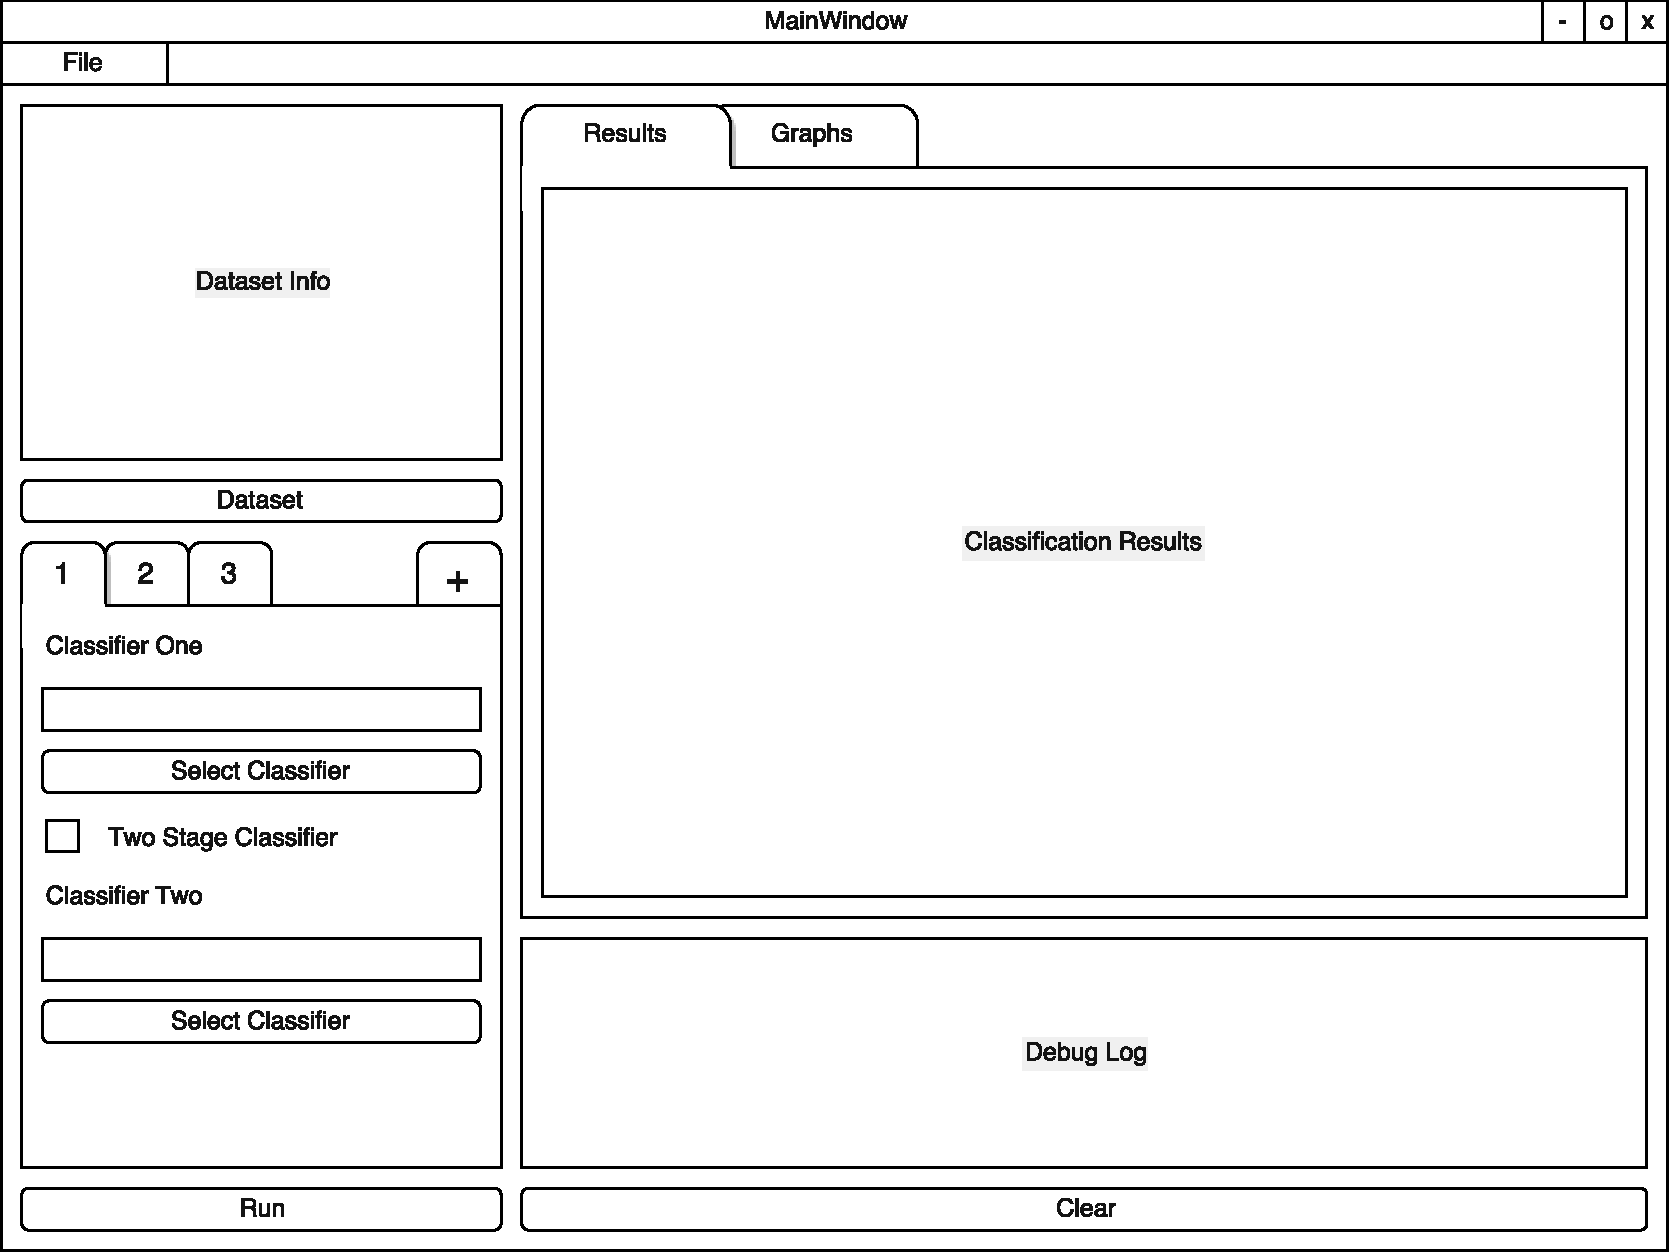
\includegraphics[width=\textwidth, center]{figures/Mainwindow.pdf}}
\caption{Main Window Result Tab Wireframe}
\label{mainwf}
\end{figure}
\begin{figure}[H]
	\makebox[\textwidth][c]{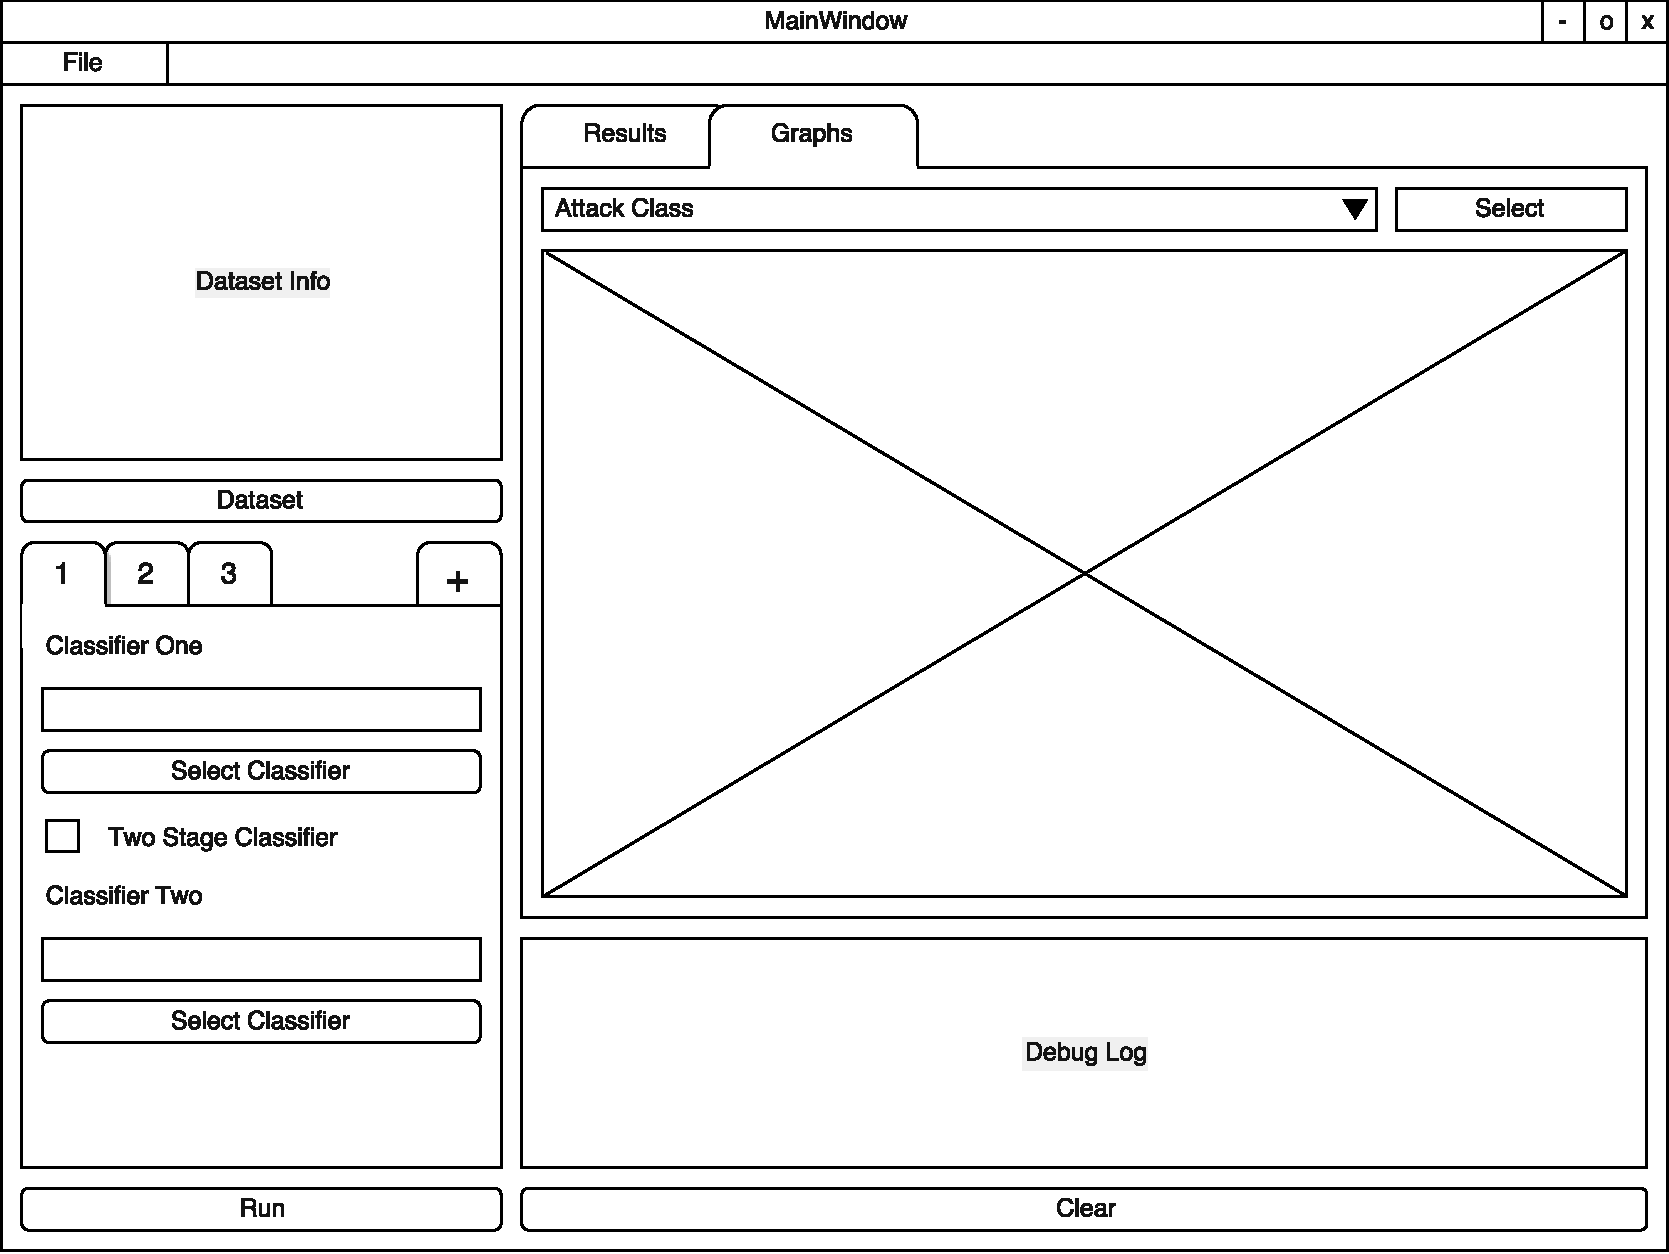
\includegraphics[width=\textwidth, center]{figures/mainwindowgraph.pdf}}
\caption{Main Window Graph Tab Wireframe}
\label{graphwf}
\end{figure}
\begin{figure}[H]
	\makebox[\textwidth][c]{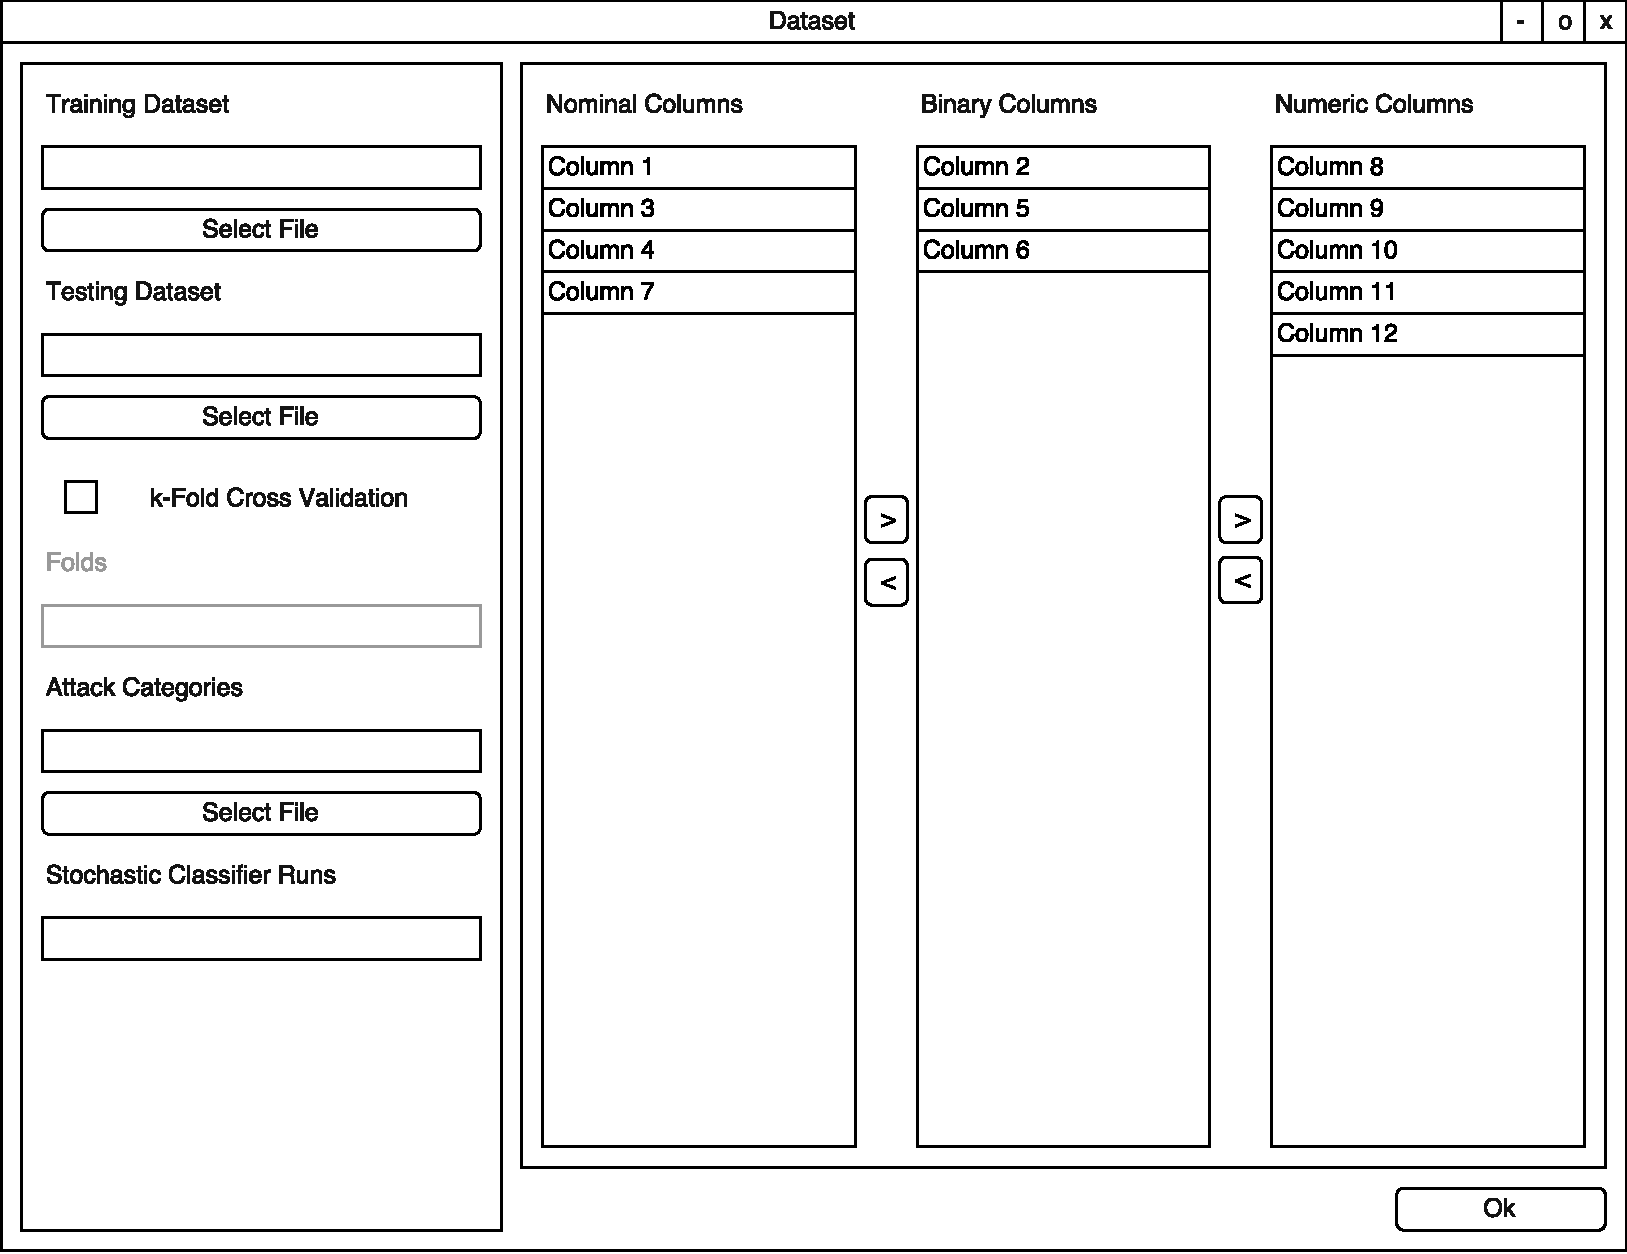
\includegraphics[width=\textwidth, center]{figures/datasetwindow.pdf}}
\caption{Dataset Window Wireframe}
\label{datasetwf}
\end{figure}

\subsubsection{Functional Requirements}
\paragraph*{FR1 - Select Classifiers}
\textbf{ID:} FR1 \\
\textbf{TITLE:} Select Classifiers \\
\textbf{PRIORITY:} High \\
\textbf{DESC:}   \\
\textbf{DEP:} N/A
\paragraph*{FR2 - Two Stage Classification}
\textbf{ID:} FR2 \\
\textbf{TITLE:} Two Stage Classification \\
\textbf{PRIORITY:} High \\
\textbf{DESC:}   \\
\textbf{DEP:} N/A
\paragraph*{FR3 - Run Classifiers}
\textbf{ID:} FR3 \\
\textbf{TITLE:} Run Classifiers \\
\textbf{PRIORITY:} High \\
\textbf{DESC:}   \\
\textbf{DEP:} FR1, FR2
\paragraph*{FR4 - Create New Classifier}
\textbf{ID:} FR4 \\
\textbf{TITLE:} Create New Classifier \\
\textbf{PRIORITY:} Low \\
\textbf{DESC:}   \\
\textbf{DEP:} N/A
\paragraph*{FR5 - Debug Output}
\textbf{ID:} FR5 \\
\textbf{TITLE:} Debug Output \\
\textbf{PRIORITY:} Medium \\
\textbf{DESC:}   \\
\textbf{DEP:} N/A
\paragraph*{FR6 - Multiple Classifier Configurations}
\textbf{ID:} FR6 \\
\textbf{TITLE:} Multiple Classifier Configurations \\
\textbf{PRIORITY:} Medium \\
\textbf{DESC:}   \\
\textbf{DEP:} FR1, FR2
\paragraph*{FR7 - Aggregate Results by Attack}
\textbf{ID:} FR7 \\
\textbf{TITLE:} Aggregate Results by Attack \\
\textbf{PRIORITY:} High \\
\textbf{DESC:}   \\
\textbf{DEP:} FR3
\paragraph*{FR8 - Write Results to File}
\textbf{ID:} FR8 \\
\textbf{TITLE:} Write Results to File \\
\textbf{PRIORITY:} Medium \\
\textbf{DESC:}   \\
\textbf{DEP:} N/A
\paragraph*{FR9 - Get Classification Results}
\textbf{ID:} FR9 \\
\textbf{TITLE:} Get Classification Results \\
\textbf{PRIORITY:} High \\
\textbf{DESC:}   \\
\textbf{DEP:} FR3
\paragraph*{FR10 - Graph Results}
\textbf{ID:} FR10 \\
\textbf{TITLE:} Graph Results \\
\textbf{PRIORITY:} High \\
\textbf{DESC:}   \\
\textbf{DEP:} FR9
\paragraph*{FR11 - Select Training Dataset}
\textbf{ID:} FR11 \\
\textbf{TITLE:} Select Training Dataset \\
\textbf{PRIORITY:} High \\
\textbf{DESC:}   \\
\textbf{DEP:} N/A
\paragraph*{FR12 - Select Testing Dataset}
\textbf{ID:} FR12 \\
\textbf{TITLE:} Select Testing Dataset \\
\textbf{PRIORITY:} High \\
\textbf{DESC:}   \\
\textbf{DEP:} N/A
\paragraph*{FR13 - k-Fold Cross Validation}
\textbf{ID:} FR13 \\
\textbf{TITLE:} k-Fold Cross Validation \\
\textbf{PRIORITY:} High \\
\textbf{DESC:}   \\
\textbf{DEP:} FR11
\paragraph*{FR14 - Select Dataset Column Labels}
\textbf{ID:} FR14 \\
\textbf{TITLE:} Select Dataset Column Labels \\
\textbf{PRIORITY:} High \\
\textbf{DESC:}   \\
\textbf{DEP:} N/A
\paragraph*{FR15 - Select Dataset Attack Categories}
\textbf{ID:} FR15 \\
\textbf{TITLE:} Select Dataset Attack Categories \\
\textbf{PRIORITY:} High \\
\textbf{DESC:}   \\
\textbf{DEP:} N/A
\paragraph*{FR16 - Categorise Dataset Fields}
\textbf{ID:} FR16 \\
\textbf{TITLE:} Categorise Dataset Fields \\
\textbf{PRIORITY:} High \\
\textbf{DESC:}   \\
\textbf{DEP:} FR14
\paragraph*{FR17 - One Hot Encoding}
\textbf{ID:} FR17 \\
\textbf{TITLE:} One Hot Encoding \\
\textbf{PRIORITY:} High \\
\textbf{DESC:}  \\
\textbf{DEP:} FR18
\paragraph*{FR18 - Load Data}
\textbf{ID:} FR18 \\
\textbf{TITLE:} Load Data \\
\textbf{PRIORITY:} High \\
\textbf{DESC:}   \\
\textbf{DEP:} FR11, FR12, FR14, FR15
\paragraph*{FR19 - k-Nearest Neighbour Classifier}
\textbf{ID:} FR19 \\
\textbf{TITLE:} k-Nearest Neighbour Classifier \\
\textbf{PRIORITY:} High \\
\textbf{DESC:}   \\
\textbf{DEP:} N/A
\paragraph*{FR20 - Multi-layer Perceptron Classifier}
\textbf{ID:} FR20 \\
\textbf{TITLE:} Multi-layer Perceptron Classifier \\
\textbf{PRIORITY:} High \\
\textbf{DESC:}   \\
\textbf{DEP:} N/A
\paragraph*{FR21 - Negative Selection Classifier}
\textbf{ID:} FR21 \\
\textbf{TITLE:} Negative Selection Classifier \\
\textbf{PRIORITY:} High \\
\textbf{DESC:}   \\
\textbf{DEP:} N/A
\paragraph*{FR22 - Support Vector Machine Classifier}
\textbf{ID:} FR22 \\
\textbf{TITLE:} Support Vector Machine Classifier \\
\textbf{PRIORITY:} High \\
\textbf{DESC:}   \\
\textbf{DEP:} N/A
\paragraph*{FR23 - Stochastic Classifier Averaging}
\textbf{ID:} FR23 \\
\textbf{TITLE:} Stochastic Classifier Averaging \\
\textbf{PRIORITY:} High \\
\textbf{DESC:}   \\
\textbf{DEP:} FR1, FR2
\paragraph*{FR24 - Feature Selection}
\textbf{ID:} FR24 \\
\textbf{TITLE:} Feature Selection \\
\textbf{PRIORITY:} Low \\
\textbf{DESC:}   \\
\textbf{DEP:} N/A

\subsubsection{Non-Functional Requirements}
\paragraph*{QR1 - Robustness}
\textbf{ID:} QR1 \\
\textbf{TITLE:} Robustness \\
\textbf{PRIORITY:} High \\
\textbf{DESC:}   \\
\paragraph*{QR2 - Responsiveness} 
\textbf{ID:} QR2 \\
\textbf{TITLE:} Responsiveness \\
\textbf{PRIORITY:} Medium \\
\textbf{DESC:} UI should not hang during stuff.   \\
\paragraph*{QR3 - Usability}
\textbf{ID:} QR3 \\
\textbf{TITLE:} Usability \\
\textbf{PRIORITY:} Medium \\
\textbf{DESC:}   \\
\paragraph*{QR4 - Maintainability}
\textbf{ID:} QR4 \\
\textbf{TITLE:} Maintainability \\
\textbf{PRIORITY:} High \\
\textbf{DESC:}   \\
\paragraph*{QR5 - Portability}
\textbf{ID:} QR5 \\
\textbf{TITLE:} Portability \\
\textbf{PRIORITY:} Low \\
\textbf{DESC:} Work on different systems and OS's  \\
\paragraph*{QR6 - Correctness}
\textbf{ID:} QR6  \\
\textbf{TITLE:} Correctness \\
\textbf{PRIORITY:} High \\
\textbf{DESC:} Results MUST be correct.   \\

\subsection{Testing}
Paragraph about testing, unit testing and why
%\begin{table}[h]
%\centering
%\caption{Test Case Descriptions}
%\label{my-label}
\begin{scriptsize}
\begin{longtable}{@{}p{0.04\textwidth}p{0.17\textwidth}p{0.17\textwidth}p{0.17\textwidth}p{0.14\textwidth}p{0.15\textwidth}@{}}
\caption{Test Case Descriptions}\\
\label{testcasetabel}\\
\toprule
ID & Objective & Precondition & Steps & Test Data & Expected \newline Result \\ \midrule
TC1 & Create new classifier tab & There is only one tab in the classifier tab box. & - Press the '+' button above the classifier tab box. & N/A & A new tab is created with the number 2 on it. \\
TC2 & Open dataset window. & N/A & - Press the 'Select Dataset..' button in the main window. & N/A & Dataset window is shown. \\ 
TC3 & Select training dataset. & Dataset window is open. & - Press the 'Select Training Set..' button. \newline - Select a file. & Any .csv file. & Absolute path of the file appears in the textbox below 'Training Dataset' label. \\ 
TC4 & Deselect k-Fold Cross Validation. & Dataset window is open and k-Fold Cross Validation checkbox is checked. & - Press the k-Fold Cross Validation checkbox. & N/A & Testing dataset label, textbox and button become enabled and folds spinbox is disabled. \\ 
TC5 & Select testing dataset. & Dataset window is open. & - Press the 'Select Testing Set...' button. \newline - Select a file. & Any valid .csv file. &  Absolute path of the file appears in the textbox below 'Training Dataset' label.\\ 
TC6 & Select dataset fields. & Dataset window is open.  &  - Press the 'Select Dataset Fields' button. \newline - Select a file.&  A .csv file containing two columns, the second of which is one of the values: Numeric, Nominal, Binary. &  Absolute path of the file appears in the textbox below 'Dataset Fields' label, and the 'Numeric', 'Nominal', and 'Binary' list views are populated.\\ 
TC7 & Select attack categories. & Dataset window is open. & - Press the 'Select Attack Categories' button. \newline - Select a file. &  Any valid .csv file.&  Absolute path of the file appears in the textbox below 'Attack Categories' label.\\ 
TC8 & Display dataset info in main window. & Valid dataset files have been selected and dataset window is open. & - Press the OK button in the bottom right of the dataset window. & N/A & The dataset window closes, showing no error message and the textbox in the top left of the main window is populated with information regarding the dataset. \\ 
TC9 & Select classifier. & N/A & - Press the 'Select Classifier' button below the 'Classifier One' label. \newline - Select a file. & Any .py file. & Absolute path of the file appears in the textbox below the 'Classifier One' label. \\ 
TC10 & Select two stage classification. & Two stage classification checkbox is unchecked. & - Press the 'Two Stage Classification' checkbox. & N/A & The 'Second Classifier' label, textbox, and 'Select Classifier' button are enabled. \\ 
TC11 & Select second classifier. & The 'Two Stage Classification' checkbox is checked. & - Press the 'Select Classifier' button below the 'Classifier Two' label. \newline - Select a file. & Any .py file. & Absolute path of the file appears in the textbox below the 'Classifier One' label. \\ 
TC12 & Error message on invalid training dataset filename. & N/A & - Enter a filepath which does not exist into the textbox below the 'Training Dataset' label. \newline - Supply every other textbox with valid filepaths. \newline - Press the OK button in the bottom right of the dataset window. & N/A & An error message is shown and the window does not exit. \\ 
TC13 & Error message on invalid testing dataset filename. & N/A & - Enter a filepath which does not exist into the textbox below the 'Testing Dataset' label. \newline - Supply every other textbox with valid filepaths. \newline - Press the OK button in the bottom right of the dataset window. & N/A & An error message is shown and the window does not exit. \\ 
TC14 & Error message on invalid field names filename. & N/A & - Enter a filepath which does not exist into the textbox below the 'Dataset Fields' label. \newline - Supply every other textbox with valid filepaths. \newline - Press the OK button in the bottom right of the dataset window. & N/A & An error message is shown and the window does not exit. \\ 
TC15 & Error message on invalid attack categories filename. & N/A & - Enter a filepath which does not exist into the textbox below the 'Attack Categories' label. \newline - Supply every other textbox with valid filepaths. \newline - Press the OK button in the bottom right of the dataset window. & N/A & An error message is shown and the window does not exit. \\ 
TC16 & Error message on invalid training dataset. & Valid dataset files have been selected, except from training dataset which is invalid. A valid classifier configuration has been selected. & - Press the 'Run' button on the main window. & N/A & An error message is displayed and the program does not crash. \\ 
TC17 & Error message on invalid testing dataset. & Valid dataset files have been selected, except from testing dataset which is invalid. A valid classifier configuration has been selected. & - Press the 'Run' button on the main window. & N/A & An error message is displayed and the program does not crash. \\ 
TC18 & Error message on invalid field names. & Valid dataset files have been selected, except from dataset fields which do not correspond to the dataset. A valid classifier configuration has been selected. & - Press the 'Run' button on the main window. & N/A & An error message is displayed and the program does not crash. \\ 
TC19 & Error message on invalid attack categories. & Valid dataset files have been selected, except from attack categories which do not correspond to the dataset. A valid classifier configuration has been selected. & - Press the 'Run' button on the main window. & N/A & An error message is displayed and the program does not crash. \\ 
TC20 & Dataset window is populated with existing information. & Dataset file paths have been previously selected and the OK button pressed on the dataset window. & - Press the 'Select Dataset..' button on the main window. & N/A & The text boxes containing the paths to files should all be filled with the information which was entered previously, as well as fold count and stochastic classifier run count. \\ 
TC21 & Error message on invalid classifier. & N/A & - Press the 'Select Classifier' button the main window. \newline - Select an invalid .py file. \newline - Press the 'Run' button. & An invalid .py file. & An error message is displayed and the program does not crash. \\ 
TC22 & Delete classifier tab. & There is more than one tab in the classifier tab. & - Press the 'x' button next to the tab number in the classifiers tabs in any tab except the first. & N/A & The tab in which the 'x' button was pressed should close. \\ 
TC23 & Show results for all classifiers run. & Valid dataset has been selected and valid classifier configuration has been selected. & - Press the 'Run' button. & N/A & A tab should be created on the main tab container for each classifier configuration run, and populated with classification information. \\ 
TC24 & Show graph of classification results. & Classifiers have been run and results retrieved. & - Select the 'Graphs' tab on the main window. \newline - Select a class from the drop down in the 'Graphs' tab. \newline - Press the 'Show' button. & N/A & A graph is shown which has a series for each classifier configuration specified. \\ 

 \bottomrule
\end{longtable}
\end{scriptsize}
%\end{table}


\section{Methodology}
\subsection{Implementation}
\subsubsection{PyQt}
PyQt is a set of Python bindings for the Qt application framework, which facilitates the writing of cross platform Qt applications which are capable of running on Windows, Mac, and Linux \parencite{pyqt5}.

PyQt was chosen as the framework of choice for creating the application GUI over other frameworks such as Java Swing for a number of reasons, the greatest of which being that it would allow all development to be carried out in Python as the libraries which were already selected for machine learning were written in Python. Writing the entire project in one language comes with extra benefits such as being able to have a single development environment, simplifying application design as there is no need for interfaces between each language, and having the ability to write all unit tests in a single language. PyQt also has powerful tools which aid in the design and development of user interfaces in the form of Qt Creator, which increased the speed of development substantially, as well as an extensive set of online documentation.

\subsubsection{Scikit-Learn}
Scikit-Learn is a Python library consisting of a set of tools for easily performing machine learning and data analysis \parencite{scikit}. The library consists of a large number or pre-implemented classification, and preprocessing algorithms, as well as others such as clustering, regression etc. These pre-implemented algorithms allowed for a much faster development cycle and also guaranteed the correctness of all algorithms which were used, again speeding up development time by removing the need for testing individual algorithms. Sci-kit also provides some basic preprocessing in the form of scaling of inputs so that they are all within a normalised range, as well as some reporting which can be used to quickly extract a lot of information in the form of confusion matrices and classification reports from the results.
	
	Some other libraries were considered for implementing the machine learning algorithms such as Tensorflow due to it's highly configurable nature and high performance due to having GPU acceleration, however the implementations of similar algorithms are considerably more complex using Tensorflow, and as time was a major factor in this project Scikit-learn was the preferable library. One final factor which influenced this choice is Scikit-learn's interoperability with Matplotlib allowing for graphs to be created quickly and easily.

\subsubsection{Pandas}
Pandas is a library which provides high performance, simple data structures and data analysis tools for Python \parencite{pandas}. Pandas provides to the programmer the DataFrame object type which allows for highly complex data manipulation to be carried out easily, such as data alignment and handling of missing data, dataset slicing, indexing and subsetting, merging and joining of multiple sets of data, etc. and is highly optimised for speed as the critical code within the library is written in C, allowing for much higher performance when compared to Python. This means that when working with very large datasets, such as the NSL-KDD and UNSW-NB15 which both have around 100,000 rows of data each, manipulations can be carried out quickly. The documentation for Pandas is also extensive and there exists a large online community of users which is indispensable during the learning of and development within the library.

\subsubsection{Matplotlib}
Matplotlib \parencite{matplotlib} is a Python 2D plotting library which produces high quality graphs and charts in both hardcopy and interactive formats. Matplotlib makes creating complex charts extremely simple as well as offering a massive number of charts, including, histograms, bar charts, scatterplots, confusion matrices, etc., with as little lines of code as possible. One large reason for selecting Matplotlib for use is its interoperability with the other libraries and frameworks which were selected. It works with Scikit-learn with very little effort and also contains custom widgets for use with PyQt which allows for extremely fast and easy integration of Matplotlib charts into the user interface of the software.

\subsubsection{Software}
The software which was written is described with a class diagram, seen in Appendix \ref{classdiagram} specifying each distinct class created along with its methods, properties and relationship with other classes, and with a use case diagram showing the general function of the software from the perspective of the user, as seen in Appendix \ref{usecase}. A description of all of the software classes functions is as follows.
\paragraph{MainWindow}
The MainWindow class is the class which is responsible for all of the logic behind the user interface of the main window. It inherits the QMainWindow class; a PyQt type which provides a main application window, and from Ui\_MainWindow, which provides the specification and initialisation of the user interface. The classes main function is handling user input, creating new user interface elements and windows, and allowing the user to view classification results.
\paragraph{DatasetWindow}
The DatasetWindow class is primarily responsible for defining what dataset the user wishes to use, to specify the data type of each column of said dataset. The window also allows users to choose between a testing dataset or k-fold cross validation and specify a number of folds, and to specify the number of runs a stochastic classifier should be run for. This class inherits from QDialog which provides the class with buttons allowing the user to accept or cancel the information they have input. It also inherits from Ui\_DatasetWindow which like Ui\_MainWindow provides the user interface for the window.
\paragraph{UIObject}
UIObject is an interface which is used by other classes which implement a user interface for some window. It is required as when a user interface is inherited by a window class a number of methods are expected to be available in order to create and render the user interface at runtime.
\paragraph{Classifier}
Classifier is an interface which any classification algorithm which is to be used must implement. It has one property, 'stochastic', which determines whether or not the classifier must be run multiple times, and a 'run' method which carries out the classification and returns the results.
\paragraph{QClfSelector}
QClfSelector is a class which inherits from QWidget, the base class of all Qt user interface objects, and who's main function is to act as a widget that can be included within MainWindow multiple times. It provides the functionality of accepting user classifier arrangements and then fetching and running those classifiers, using whatever method has been specified by the user, be it k-fold cross validation or using a test dataset, or running stochastic classifiers multiple times and gathering the results.
\paragraph{QBarChart}
QBarChart is a class which inherits from 'FigureCanvas', a Matplotlib class which interfaces with PyQt in order to create widget which can be displayed within a PyQt application. The class accepts a set of classification results and then constructs a Matplotlib chart which can be displayed in the MainWindow class for the user to view.
\paragraph{ErrorMessage}
The ErrorMessage Class is the class responsible for displaying an error message popup to users, in a standard manner and encapsulates boiler plate code required for creating and showing a message box. The class inherits from QMessageBox which is a PyQt class provides a modal dialog for informing the user.
\subsection{Datasets}
\subsubsection{NSL-KDD}
Within the KDD-NSL dataset, traffic is categorised into either normal network traffic for a military network or into one of the following four attack categories:
\begin{itemize}
\item{Denial of Service (DoS) - Attacker tries to prevent legitimate users from using a service.}
\item{Remote to Local (r2l) - Attacker does not have an account on the victim machine, hence tries to gain access.}
\item{User to Root (u2r) - Attacker has local access to the victim machine and tries to gain super user privileges.}
\item{Probe - Attacker tries to gain information about the target host.}
\end{itemize}
A complete listing of all attacks and their categories can been seen in Table \ref{nslkddattacksamples}, as well as the sample count of each category of attack in Table \ref{nslkddsamples}.
\begin{longtable}{@{}ccc@{}}
\caption{NSL-KDD Dataset Attack Samples.} \\
\label{nslkddattacksamples} \\
\toprule
Attack & Samples & Category  \\
\midrule
back & 956 & dos \\ 
buffer\_overflow & 30 & u2r \\ 
ftp\_write & 8 & r2l \\ 
guess\_passwd & 53 & r2l \\ 
imap & 11 & r2l \\ 
ipsweep & 3599 & r2l \\ 
land & 18 & dos \\ 
loadmodule & 9 & u2r \\ 
multihop & 7 & r2l \\ 
neptune & 41214 & dos \\ 
nmap & 1493 & probe \\ 
normal & 67343 & normal \\ 
perl & 3 & u2r \\ 
phf & 4 & r2l \\ 
pod & 201 & dos \\ 
portsweep & 2931 & probe \\ 
rootkit & 10 & u2r \\ 
satan & 3633 & probe \\ 
smurf & 2646 & dos \\ 
spy & 2 & r2l \\ 
teardrop & 892 & dos \\ 
warezclient & 890 & r2l \\ 
warezmaster & 20 & r2l \\ 
\bottomrule
\end{longtable}

\begin{table}[H]
\centering
\caption{NSL-KDD Dataset Categories Samples.}
\label{nslkddsamples}
\begin{tabular}{@{}ccccc@{}}
\toprule
DoS & Probe & u2r & r2l & Normal  \\
\midrule
45927 & 11656 & 52 & 995 & 67343 \\ 
\bottomrule
\end{tabular}
\end{table}


The dataset itself is also comprised of 41 features per connection recorded, a detailed listing of each and their type can be seen in Appendix \ref{kddfeatures}.

\subsubsection{UNSW-NB15}
Similarly, within the UNSW-NB15 dataset, as with the NSL-KDD dataset, traffic is also categorised into either normal network traffic for a military network or into one of the following seven attack categories:
\begin{itemize}
	\item{Fuzzers - Attempting to cause a program or network suspended by feeding it the randomly generated data. Analysis 2,677 It contains different attacks of port scan, spam and html files penetrations.}
	\item{Backdoors - A tecnique in which a system security mechanism is bypassed stealthily to access a computer or its data.}
	\item{DoS - A malicious attempt to make a server or a network resource unavailable to users, usually by temporarily interrupting or suspending the services of a host connected to the Internet.}
	\item{Exploits - The attacker knows of a security problem within an operating system or a piece of software and leverages that knowledge by exploiting the vulnerability.}
	\item{Generic - A technique works against all block-ciphers (with a given block and key size), without consideration about the structure of the block-cipher.}
	\item{Reconnaissance - Contains all Strikes that can simulate attacks that gather information.}
	\item{Shellcode - A small piece of code used as the payload in the exploitation of software vulnerability. Worms 174 Attacker replicates itself in order to spread to other computers. Often, it uses a computer network to spread itself, relying on security failures on the target computer to access it.}
\end{itemize}
\begin{longtable}{@{}ccc@{}}
\caption{UNSW-NB15 Dataset Attack Samples.} \\
\label{unswattacks} \\
\toprule
Attack & Samples \\
\midrule
Analysis & 677 \\
Backdoor & 583 \\
DoS & 4089 \\
Exploits & 11132  \\
Fuzzers & 6062 \\
Generic & 18871\\
Reconnaissance & 3496 \\
Shellcode & 378\\
Worms & 44 \\
Normal & 37000 \\
\bottomrule
\end{longtable}

	The UNSW-NB15 dataset is comprised of 42 features per connection recorded, a detailed listing of each feature, their type and a description of each can be seen in Appendix \ref{unswfeatures}.
\subsection{Data Pre-processing}
Before classification can take place it is necessary to perform some pre-processing upon both datasets, so that when they are used they are in a form which is most useful for classification, allowing for more accurate, and faster classification. The first form of pre-processing which will take place upon the datasets is in the form of one hot encoding. One hot encoding is a process wherein categorical features of a dataset are converted into a binary representation. This process can be seen in Figure \ref{ohe}, which shows a small snippet from the NSL-KDD dataset before, and after one hot encoding.

\begin{figure}[H]
\begin{adjustbox}{width=1.0\textwidth,center}
\begin{tabular}{ccc}
\hline
flag&src\_bytes&dst\_bytes\\
\hline
SF&491&0\\
SF&146&0\\
S0&0&0\\
SF&232&8153\\
SF&199&420\\
REJ&0&0\\
\hline
\end{tabular}
\quad
\longrightarrow
\quad
\begin{tabular}{ccccc}
\hline
flag\_SF&flag\_S0&flag\_REJ&src\_bytes&dst\_bytes\\
\hline
1&0&0&491&0\\
1&0&0&146&0\\
0&1&0&0&0\\
1&0&0&232&8153\\
1&0&0&199&420\\
0&0&1&0&0\\
\hline
\end{tabular}
\end{adjustbox}
\caption{One-hot Encoding Example}
\label{ohe}
\end{figure}



%REWRITE THIS, EXPLAIN ONEHOT BECAUSE OF AVERAGING NOT DISTANCE
One hot encoding is necessary as many classification algorithms rely on either some kind of internal averaging, or some form of activation function which require numerical input in order to extract meaning from. Simply converting each of these categories from a nominal to a numeric representation is not sufficient as the categories lose meaning when represented by a series of numbers, i.e. when calculating distance from one category to another any number selected will be arbitrary, and the machine learning algorithm will attempt to extract a relationship between the numbers where there is none, therefore reducing accuracy in classification. 

One side effect of one hot encoding is that when processing both the training and testing dataset it is possible that the testing set is missing some categories present within the training set, leading to the algorithms being unable to perform a categorisation. To rectify this the next form of pre-processing which must take place is the insertion of missing features from the training set into the testing set. To do this the training set is simply scanned to find features which are not present in the testing set, and then inserts them into the testing set at the same index thereby making both sets features identical.

The final form of pre-processing to be performed on the dataset is feature scaling. Feature scaling is where a range of data is normalised by scaling it to be within some range, in this case between -1 and 1. The formula used for doing this is seen below in Figure \ref{scale}:
\begin{figure}[H]
	\[ x' = \frac{x - min(x)}{max(x) - min(x)} \] 
\caption{Feature Scaling Formula}
\label{scale}
\end{figure}
where $ x $ is the original value and $ x' $ is the normalised value. Representing a range of values between a normalised range is important as a large number of classification algoithms compute the euclidian distance between two points and will therefore not work correctly if two different featues have wildy different scales. For example if one feature has a large range of numbers and another a very narrow range, the distance will be dependant only on the feature with the larger range, so each feature should be normalised to ensure that each contributes the same amount to the final distance which is computed. Feature scaling also allows classifers which use gradient descent, such as the multi-layer perceptron, to converge much faster allowing for faster collection of results.
\subsection{Classifier Configurations}
The following is a listing of the parameters used in the running of each of the classifiers implemented within the scikit-learn library, with the descriptions of each taken from the official documentation:

% Please add the following required packages to your document preamble:
% \usepackage{booktabs}
\begin{small}
\begin{longtable}{@{}p{2cm}p{2.5cm}p{1.6cm}p{1.6cm}p{4.5cm}@{}}
\caption{Classifier Parameters} \\
\label{params} \\
\toprule
& Parameter & NSL-KDD Value & UNSW-NB15 Value & Description \\ \midrule
k-Nearest Neighbour & algorithm & 'kdtree' & 'kdtree' & Algorithm used to compute the nearest neighbors. \\
    & weights & 'uniform' & 'uniform' & Uniform weights. All points in each neighborhood are weighted equally. \\
    & leaf\_size & 40 & 40 & Leaf size used for the KDTree. \\
    & p & 2 & 2 & Power parameter for the Minkowski metric. \\
 & n\_neighbors & 3 & 2 & The number of nearest neighbours to search for, i.e. $k$. \\
Multi-Layer Perceptron & hidden\_layer \_sizes & 100 & 100 & The number of neurons within the hidden layer. \\
		       & activation & 'relu' & 'relu & Activation function for the hidden layer, rectified linear unit function, returns \newline $ f(x) = max(0, x) $. \\
	 & solver & 'adam' & 'adam' & The solver for weight optimization, ‘adam’ refers to a stochastic gradient-based optimizer proposed by \cite{kingma2014adam}. \\
  & learning\_rate & 'invscaling' & 'invscaling & The learning schedule, ‘invscaling’ gradually decreases the learning rate at each time step. \\
Support Vector Machine & kernel & 'rbf' & 'rbf' & Specifies the kernel type to be used in the algorithm, Radial Basis Function kernel. \\
		       & gamma & $ 1e-1 $ & $ 1e-1 $ & How much influence a single training example has. The larger gamma is, the closer other examples must be to be affected. \\
	 & C & 10 & 10 & Trades off misclassification of training examples against simplicity of the decision surface. A low C makes the decision surface smooth, while a high C aims at classifying all training examples correctly. \\ \bottomrule
\end{longtable}
\end{small}


\subsection{Single Stage Classification}
The first form of classification which will take place is single stage classification. In single stage classification only a single machine learning technique and stage is implemented in order to classify network traffic. The dataset is first read and preprocessed, and the entire set is used in order to train the machine learning classifier. One the classifier has been trained, the classifier will make predictions about the testing set, classifying it into normal traffic or any one of the attack categories for the dataset it was trained upon, e.g. the attacks seen in Table \ref{nslkddattacksamples}.

\subsection{Two Stage Classification}
In second form of classification to take place is two stage classification. In two stage classification, the classification processes is split into two separate stages, the first indentifying normal traffic, and the second identifying abnormal. Before the first stage is trained, the dataset must first be flattened, with all attack types being reduced to simply 'attack', resulting in a set of data labelled only 'normal' and 'attack'. This new dataset is then used to train the first classifier, and then predictions made about the testing set, consisting of only 'normal' and 'attack' classifications. The second classifier is now trained on the original, unflattened dataset with all of the normal traffic removed, resulting in a dataset consisting of only attacks. Once the classifier has been trained, the traffic which was classified as being an attack by the first classifier is then fed into the second classifier, and is then labelled as a specific attack. The total result is then the combination of the traffic identified as normal within the first classifier and the attacks from the second classifier. 

	Performing classification in this manner is expected to give more accurate results than a single stage classifier as it allows each stage to specialise, with the first only needing to differentiate between two classes, 'normal' and 'attack', and the second stage focussed on specific attack types, in theory increasing the overall rate of accurate detection by reducing domain size.

\subsection{Data Collection}
When performing data collection a number of things were done to ensure the greatest consistency within the results gathered, that comparisons between classification methods are valid, and that the results portray the real world performance of such a classifier as closely as possible. The first thing done to ensure validity of results gathered is that classifiers which are stochastic, i.e. are non-deterministic, are run for a total of 30 times and the results are averaged to reduce the amount of randomness within the results and lower the chance that a classifier may perform abnormally well or otherwise.

	% Please add the following required pac$k_ages to your document preamble:
% \usepac$k_age{boo$k_tabs}
\begin{figure}[H]
\centering
\caption{k-Fold Cross Validation}
\label{kfold}
\begin{tabular}{@{}cllllllllll@{}}
\toprule
\multicolumn{1}{l}{Iteration} & \multicolumn{10}{c}{Dataset} \\ \midrule
\multicolumn{1}{c}{1} & \cellcolor{lightgray} $k__1$ & $k_2$ & $k_3$ & $k_4$ & $k_5$ & $k_6$ & $k_7$ & $k_8$ & $k_9$ & $k_1_0$ \\
\multicolumn{1}{c}{2} & $k_1 & \cellcolor{lightgray}$k_2$ & $k_3$ & $k_4$ & $k_5$ & $k_6$ & $k_7$ & $k_8$ & $k_9$ & $k_1_0$ \\
\multicolumn{1}{c}{3} & $k_1 & $k_2$ & \cellcolor{lightgray}$k_3$ & $k_4$ & $k_5$ & $k_6$ & $k_7$ & $k_8$ & $k_9$ & $k_1_0$ \\ 
 \multicolumn{1}{c}{\vdots} &  &  &  &  &  \multicolumn{1}{c}{\vdots} &  &  &  &  &  \\ 
\multicolumn{1}{c}{9} & $k_1 & $k_2$ & $k_3$ & $k_4$ & $k_5$ & $k_6$ & $k_7$ & $k_8$ & \cellcolor{lightgray}$k_9$ & $k_1_0$ \\
\multicolumn{1}{c}{10} & $k_1 & $k_2$ & $k_3$ & $k_4$ & $k_5$ & $k_6$ & $k_7$ & $k_8$ & $k_9$ & \cellcolor{lightgray}$k_1_0$ \\ \bottomrule
\end{tabular}
\end{figure}


To best represent the real world performance of the classifiers, k-fold cross validation was used as described by \cite{refaeilzadeh2009cross}. In k-fold cross validation the training dataset is partitioned into $ k $ equal parts, with one part being used as the testing dataset the classifier will make predictions about, and the remaining $ k-1 $ parts used as the training set. This process is repeated $ k $ times with a different fold used each time as the testing set, a diagram of which can been seen in Figure \ref{kfold}. The results from all of these folds can then be combined and used to obtain a single result for the performance of the classification method. Using this method for testing the performance of classifier is preferable to the use of a testing set as the all of the data available is used as both training data and testing data, therefore giving a more accurate estimation of how well the classifier will generalize to any independent dataset, i.e. it gives a more accurate idea of how well the classifier will perform in practice.

The k value selected for the k-fold cross validation to be carried out in this investigation is $ k=10 $ as a study carried out by \cite{kohavi1995study} found ten-fold cross validation to be the most effective in producing accurate results. The same k value was used throughout for each classifier, as well as the using the same folds for gathering results without randomising to ensure that results collected were comparable.

Finally the same parameters were used for each of the classifier arrangements, as described in Table \ref{params}, to ensure that results across classifier arrangements were consistent with one and other.

\subsection{Metrics}
\subsubsection{Precision}
\[ precision = \frac{tp}{tp+fp} \]
\subsubsection{Recall}
\[ recall = \frac{tp}{tp+fn} \]
\subsubsection{f1-Score}
\[ f_1 = \frac{2tp}{2tp+fp+fn} \]

\section{Evaulation}
\subsection{Software}
Evaluate the software
How many of the function requirements were met
How many of the non functional requirements were met
Is the user interface like it was designed
How does it compare to existing software
\subsection{k-Nearest Neighbours}
\subsection{Multi-layer Perceptron}
\subsection{Support Vector Machine}
\subsection{Single-Stage Classifiers Performance}
\subsection{Two-stage Classifiers Performance}
in knn-knn the second stage for unsw results in the same normals but removing normals mean that it cannot detect attacks as easily. In the svm-svm the normal has a lower number of true positives than the single stage, increasing false postivies within attacks.

\section{Conclusion}
\subsection{Research Questions}
\subsubsection*{What is the rate of accurate detection and classification of network intrusions by single stage machine learning classification methods?}
\subsubsection*{What is the rate of accurate detection and classification of network intrusions by two stage machine learning classification methods?}
\subsubsection*{Which method of classification i.e. single stage or two stage, is more accurate and by what amount?}
\subsubsection*{Which configuration of algorithms in the two stage classifier produces the most accurate results?}

\subsection{Has the Project met it's Aims and Objectives?}
\subsection{Reflection}
\subsection{Learning Outcomes}
\subsubsection*{LO1 - Manage a substantial individual project, including planning, documentation and control}
\subsubsection*{LO2 - Construct a focussed problem statement and conduct a suitable investigation, including literature or technology review, into the context of that problem}
\subsubsection*{LO3 - Demonstrate professional competence by applying appropriate theory and practice to the analysis, design, implementation and evaluation of a non-trivial set of deliverables}
\subsubsection*{LO4 - Show a capacity for self-appraisal by analysing the strengths and weaknesses of the project process and outcomes with reference to the initial objectives and to the work of others}
\subsection{Further Research}

\newpage
	\printbibliography
\newpage

\begin{appendices}
\section{Project Overview}

%\vspace{0.3cm}

\section*{Initial Project Overview}\\

\vspace{0.3cm}

\section*{SOC10101 Honours Project (40 Credits)} \\

\vspace{0.3cm}

\section*{Title of Project: A Comparison of Machine Learning Algorithms to Detect Network Intrusions} \\

\vspace{0.3cm}

\section*{Overview of Project Content and Milestone}
\noindent For this project, the main objective is to research different machine learning strategies for detecting network intrusions and to develop a piece of software which can obtain metrics from these algorithms. The focus of this project will be on a comparison of two-stage classifiers versus single-stage classifiers for detecting and classifying network intrusions. The dataset upon which these methods will be tested is the KDD Cup 1999 dataset, with the possibility of testing upon other data sets should time allow it. \\


\noindent The different strategies for machine learning will be gathered by reading relevant research papers and articles within the field of machine learning and network intrusion detection and selecting appropriate algorithms/strategies which are applicable for the chosen data set, and which are also feasible to implement within the timescale. \\


\noindent The software will be a desktop application and will take either a predetermined algorithm or a user submitted algorithm, and a data set of network traffic. The software should then run the algorithm and extract metrics from it such as rates for false positives, true positives, false negatives, true negatives, overall accuracy of classification, etc. These results can then be used to plot graphs and charts to visualise this information to a user in a useful way. \\


\noindent A dissertation will be delivered at the end of the project and should contain a detailed design and plan of the software as well as complete testing strategy and results. Also included in the final report should be a comparison of several of the implemented algorithms to determine which is the most suitable for use if any at all. \\

\noindent A list of milestones for this project goes as the following:
\begin{multicols}{2}
\begin{itemize}
\item{Initial Project Overview Submitted}
\item{Relevant Algorithms Selected}
\item{Project timescale Completed}
\item{Literature Review Complete}
\item{Software Design Completed}
\item{Algorithms Implemented}
\item{Software Implemented}
\item{Software Testing Plan}
\item{Software Tested}
\item{Algorithm Comparison Completed}
\item{Dissertation Written}
\item{Poster Presentation Completed}
\item{Project Submitted}
\end{itemize}
\end{multicols}

\section*{The Main Deliverable(s):}
\noindent A list of the main deliverables for the project is as follows:
\begin{multicols}{2}
	\begin{itemize}
	\item{Initial Project Overview}
	\item{Gantt Chart}
	\item{Literary Review}
	\item{Interim Report}
	\item{Requirement Specification}
	\item{Software Design Document}
	\item{Software Test Plan}
	\item{Software Test Results}
	\item{Software Implementation}
	\item{Algorithm Implementations}
	\item{Meeting Diary}
	\item{Algorithm Experimental Results}
	\item{Algorithm Comparisons}
	\item{Software User Documentation}
	\item{Dissertation}
	\item{Poster Presentation
	\end{itemize}
\end{multicols} \\


\section*{The Target Audience for the Deliverable(s):}
\noindent The target audience for this project could include, machine learning and network intrusion researchers, and computer science students. Researchers may find the comparison of algorithms to be highly useful when carrying out preliminary research and could save time on selecting or discounting an algorithm. Computer science students may also find this project of use for experimenting with different network intrusion methods and different machine learning methods, giving them an insight on what they can be used for and how effective they are. \\


\section*{The Work to be Undertaken:}
\noindent During this project, the work which must be undertaken is first extensive research of the subject area and collection of relevant sources. The project must then be planned and a timeline of work set out to be completed, with deadlines for each deliverable. Algorithms such as k-nearest neighbour, Artificial neural network, negative selection genetic algorithm, etc, will be implemented, compared and contrasted, specifically the performance of single stage against two-stage classifiers using these algorithms. At the same time as implementing these algorithms a requirement specification and then a design document will be created for the software package as well as a test plan. The design will then be implemented and then be tested according to the test plan. Once fully tested and proven correct the software can then be used to compare the algorithms and obtain metrics from then. The final dissertation will then be written which will include an analysis of the results for each algorithm. \\


\section*{Additional Information / Knowledge Required:}
\noindent Additional research is required on network intrusion and two stage classifiers to best select the methods which will be implemented and explored. Research into similar software products such as WEKA ("Weka 3 - Data Mining with Open Source Machine Learning Software in Java", 2017) will also be conducted to source ideas and to see in which areas these pieces of software are lacking. Research on each individual algorithm to be implemented will also be required to ensure a correct implementation. And finally, an investigation into relevant libraries which may be used to assist with GUI creation, Graphing, and algorithm implementations. \\


\section*{Information Sources that Provide a Context for the Project:}
\noindent 1. Tsai, C. F., Hsu, Y. F., Lin, C. Y., & Lin, W. Y. (2009). Intrusion detection by machine learning: A review. Expert Systems with Applications, 36(10), 11994-12000. \\

\noindent 2. Sommer, R., & Paxson, V. (2010, May). Outside the closed world: On using machine learning for network intrusion detection. In Security and Privacy (SP), 2010 IEEE Symposium on (pp. 305-316). IEEE. \\

\noindent 3. Denning, D. E. (1987). An intrusion-detection model. IEEE Transactions on software engineering, (2), 222-232. \\

\noindent 4. Powers, S. T., & He, J. (2008). A hybrid artificial immune system and Self Organising Map for network intrusion detection. Information Sciences, 178(15), 3024-3042. \\

\noindent 5. Shon, T., & Moon, J. (2007). A hybrid machine learning approach to network anomaly detection. Information Sciences, 177(18), 3799-3821. \\

\noindent 6. Mukkamala, S., Janoski, G., & Sung, A. (2002). Intrusion detection using neural networks and support vector machines. In Neural Networks, 2002. IJCNN'02. Proceedings of the 2002 International Joint Conference on (Vol. 2, pp. 1702-1707). IEEE. \\

\noindent 7. Frank, J. (1994, October). Artificial intelligence and intrusion detection: Current and future directions. In Proceedings of the 17th national computer security conference (Vol. 10, pp. 1-12). \\

\noindent 8. Weka 3 - Data Mining with Open Source Machine Learning Software in Java. (2017). Cs.waikato.ac.nz. Retrieved 21 September 2017, from http://www.cs.waikato.ac.nz/ml/weka/ \\

\section*{The Importance of the Project:}
\noindent This project has importance as there has not been many papers directly comparing implementations of different machine learning approaches to network intrusion detection. While there are software packages which deal with gaining metrics from and comparing algorithms there is not one which is focused solely on network intrusion detection. Making a piece of software which is focused on one area of research may prove to provide greater insights, through more focussed results or through ease of use regarding comparing single and multiple stage classifiers, whereas a more complicated piece of software may take a long time to become acquainted with and to produce results. \\


\section*{The Key Challenge(s) to be Overcome:}
\noindent The key challenges to be overcome in this project are the implementations of the machine learning algorithms themselves. This is due to a personal lack of experience in implementing machine learning algorithms. Experience is also lacked in understanding formal descriptions of algorithms which may hinder my understanding of techniques when reading research papers. Another challenge will be creating a method of accommodating algorithms by creating interfaces which they will communicate with the main piece of software allowing for any algorithm to be entered by a user.


\includepdf[pages=-]{figures/ipo}

\begin{subappendices}
\subsection{Project Timeline}

\begin{figure}[h!]
	\centering
	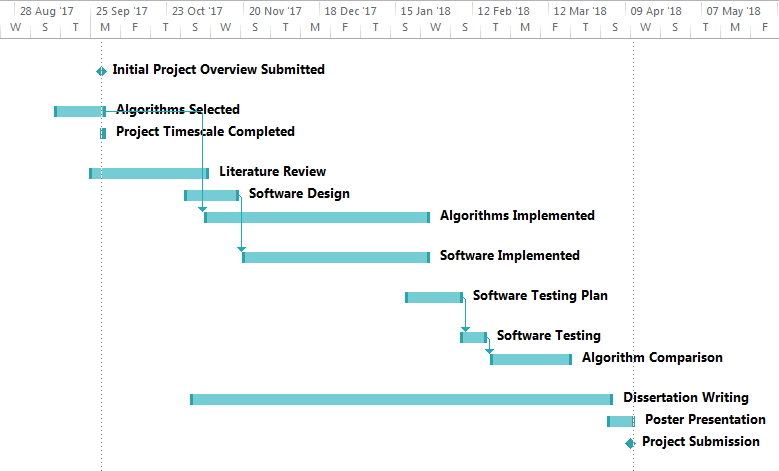
\includegraphics[width=1.11\textwidth,angle=90]{figures/Ganttchart}
	\caption{Project Timeline Gantt Chart}
	\label{gantt}
\end{figure}

\end{subappendices}

\newpage

\section{Second Formal Review Output}
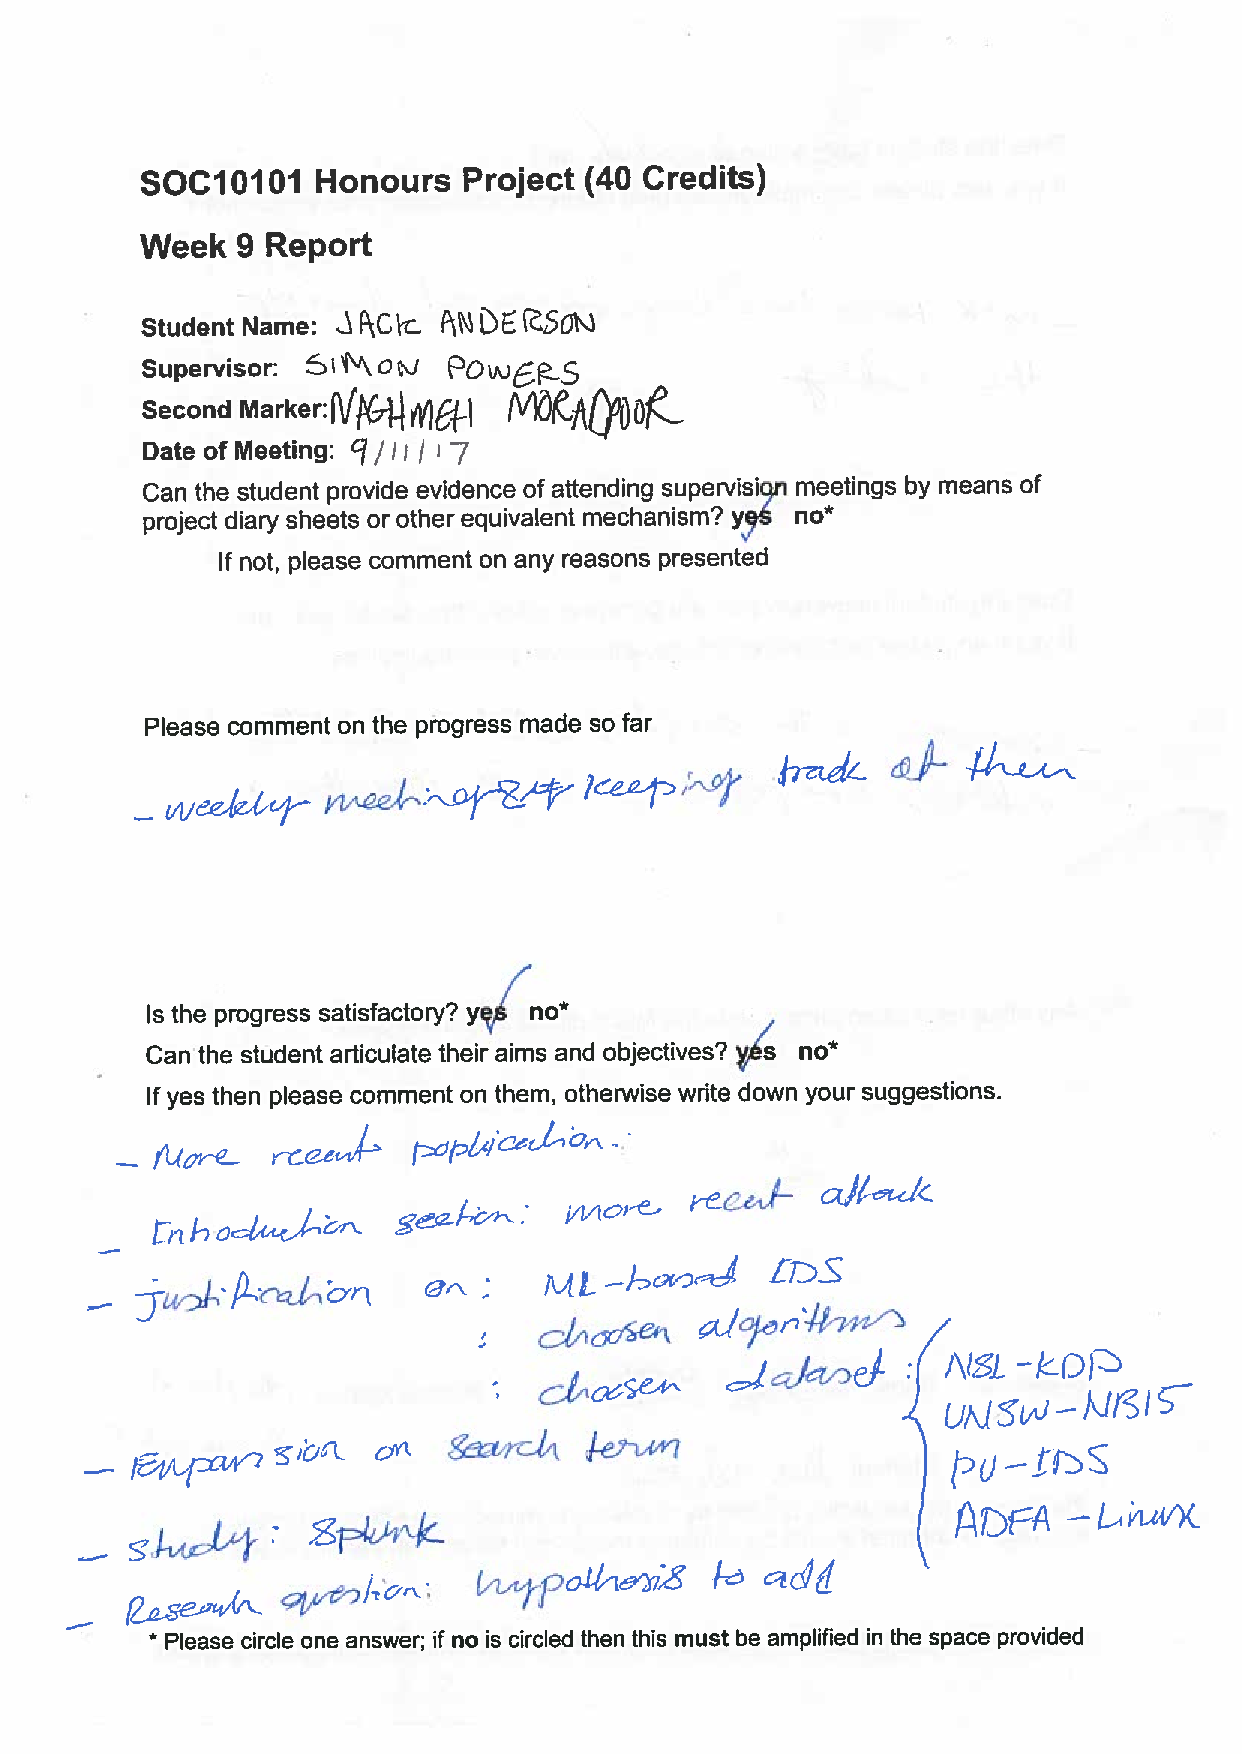
\includepdf[pages=-]{figures/interim}

\section{Diary Sheets (or other project management evidence)}
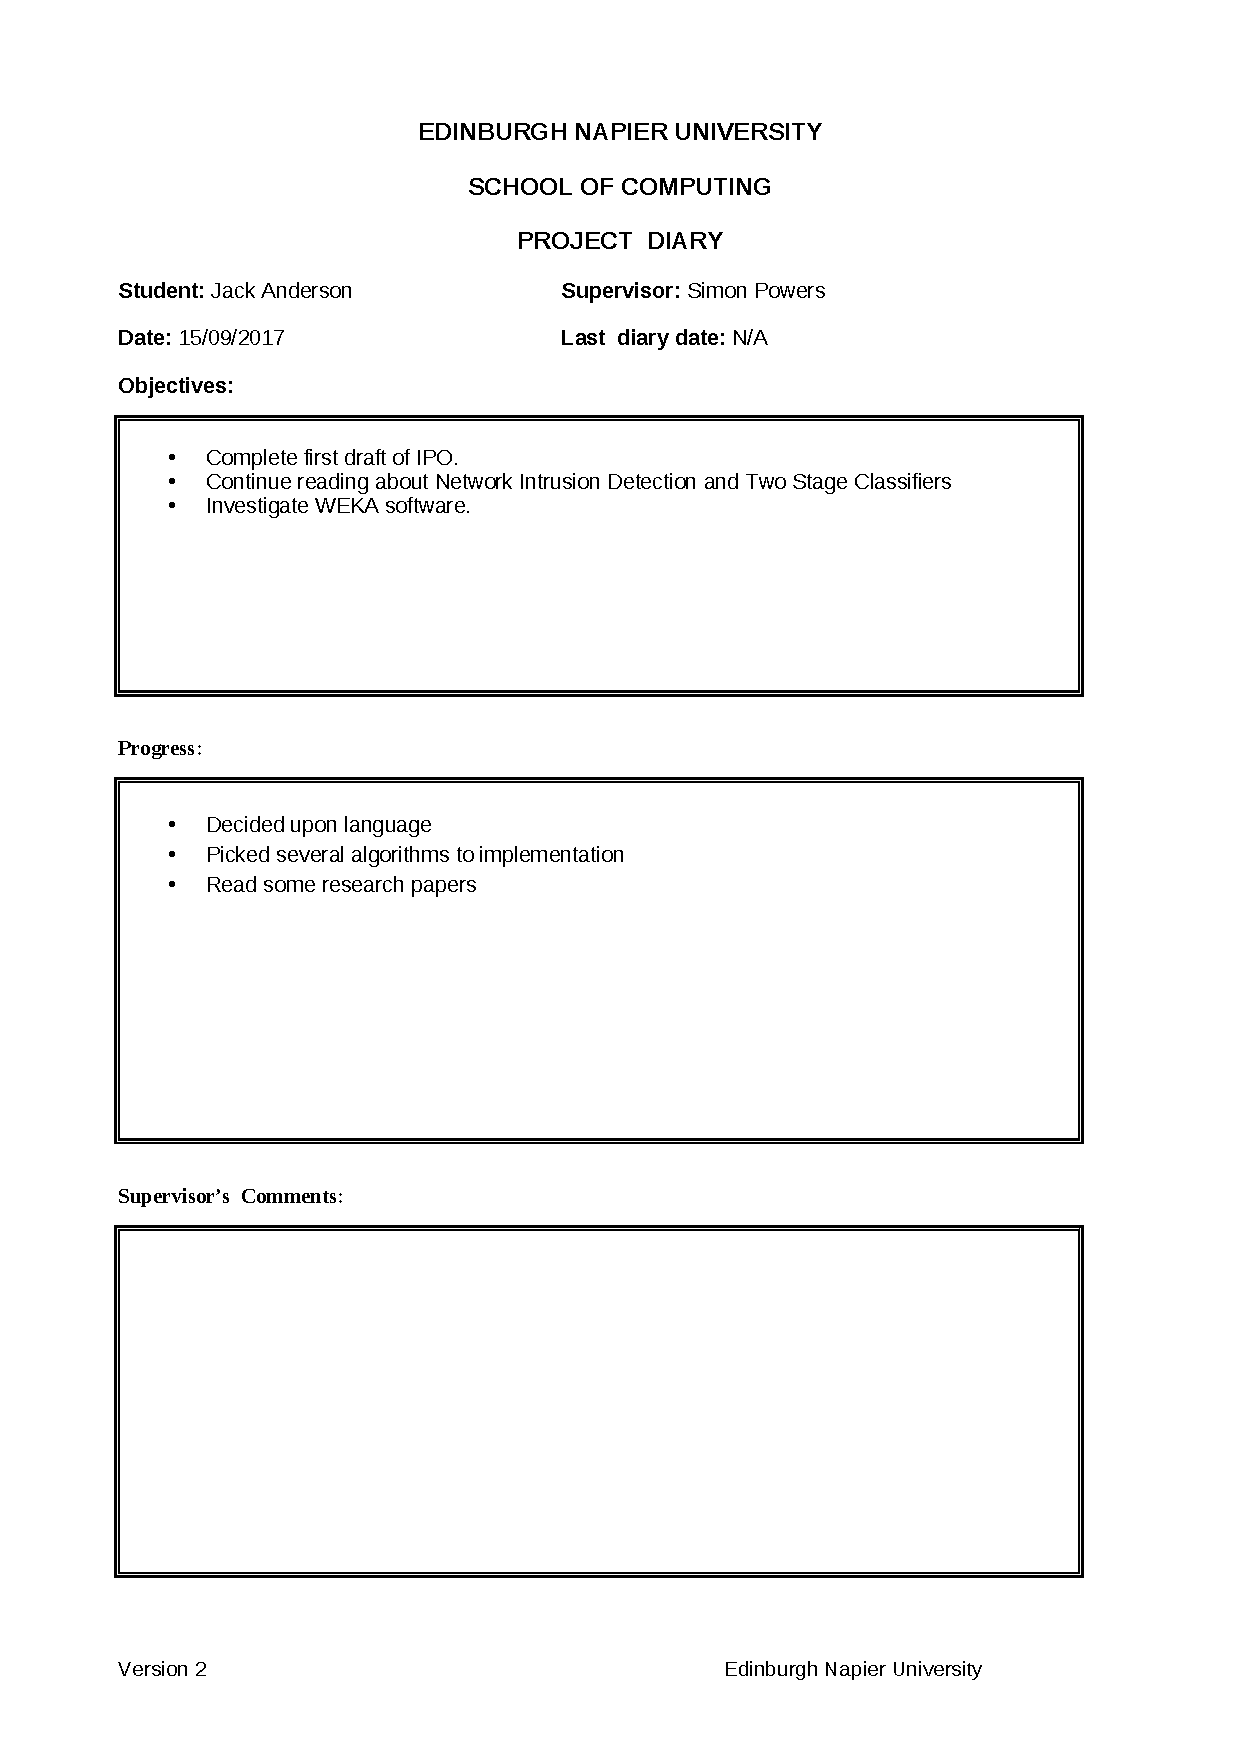
\includepdf[page=-]{figures/diaries}

\newpage

\section{MoSCoW Analysis}
\begin{table}[H]
\centering
\caption{MoSCoW Analysis of Requirements}
\label{my-label}
\begin{adjustbox}{center=\textwidth}
\begin{tabular}{@{}llcccc@{}}
\toprule
\multicolumn{2}{c}{Requirement} & \multicolumn{4}{c}{Priority} \\ 
\cmidrule(lr){1-2}
\cmidrule(lr){3-6}
ID & Title & Must & Should & Could & Wont \\ \midrule
FR1 & Select Classifiers                 & \textbf{x} & \textbf{} & \textbf{} & \textbf{} \\
FR2 & Two Stage Classification           & \textbf{x} & \textbf{} & \textbf{} & \textbf{} \\
FR3 & Run Classifiers                    & \textbf{x} & \textbf{} & \textbf{} & \textbf{} \\
FR4 & Create New Classifier              & \textbf{} & \textbf{} & \textbf{x} & \textbf{} \\
FR5 & Debug Output                       & \textbf{} & \textbf{x} & \textbf{} & \textbf{} \\
FR6 & Multiple Classifier Configurations & \textbf{} & \textbf{x} & \textbf{} & \textbf{} \\
FR7 & Aggregate Results By Attack        & \textbf{x} & \textbf{} & \textbf{} & \textbf{} \\
FR8 & Write Results to File              & \textbf{} & \textbf{x} & \textbf{} & \textbf{} \\
FR9 & Get Classification Results         & \textbf{x} & \textbf{} & \textbf{} & \textbf{} \\
FR10 & Graph Results                     & \textbf{} & \textbf{x} & \textbf{} & \textbf{} \\
FR11 & Select Training Dataset           & \textbf{x} & \textbf{} & \textbf{} & \textbf{} \\
FR12 & Select Testing Dataset            & \textbf{x} & \textbf{} & \textbf{} & \textbf{} \\
FR13 & k-Fold Cross Validation           & \textbf{x} & \textbf{} & \textbf{} & \textbf{} \\
FR14 & Select Dataset Column Labels      & \textbf{x} & \textbf{} & \textbf{} & \textbf{} \\
FR15 & Select Dataset Attack Categories  & \textbf{x} & \textbf{} & \textbf{} & \textbf{} \\
FR16 & Categorise Dataset Fields         & \textbf{x} & \textbf{} & \textbf{} & \textbf{} \\
FR17 & One Hot Encoding                  & \textbf{x} & \textbf{} & \textbf{} & \textbf{} \\
FR18 & Load Data                         & \textbf{x} & \textbf{} & \textbf{} & \textbf{} \\
FR19 & k-Nearest Neighbour Classifier    & \textbf{x} & \textbf{} & \textbf{} & \textbf{} \\
FR20 & Multi-layer Perceptron Classifier & \textbf{x} & \textbf{} & \textbf{} & \textbf{} \\
FR21 & Negative Selection Classifier     & \textbf{} & \textbf{} & \textbf{x} & \textbf{} \\
FR22 & Support Vector Machine Classifier & \textbf{x} & \textbf{} & \textbf{} & \textbf{} \\
FR23 & Stochastic Classifier Averaging   & \textbf{} & \textbf{x} & \textbf{} & \textbf{} \\
FR24 & Feature Selection                 & \textbf{} & \textbf{} & \textbf{} & \textbf{x} \\
QR1 & Robustness                         & \textbf{x} & \textbf{} & \textbf{} & \textbf{} \\
QR2 & Responsiveness                     & \textbf{} & \textbf{} & \textbf{x} & \textbf{} \\
QR3 & Usability                          & \textbf{} & \textbf{x} & \textbf{} & \textbf{} \\
QR4 & Maintainability                    & \textbf{x} & \textbf{} & \textbf{} & \textbf{} \\
QR4 & Correctness                        & \textbf{x} & \textbf{} & \textbf{} & \textbf{} \\
QR5 & Portability                        & \textbf{} & \textbf{} & \textbf{x} & \textbf{} \\ \bottomrule
\end{tabular}
\end{adjustbox}
\end{table}


\newpage

\section{Class Diagram} \label{classdiagram}
\begin{figure}[H]
	\makebox[\textwidth][c]{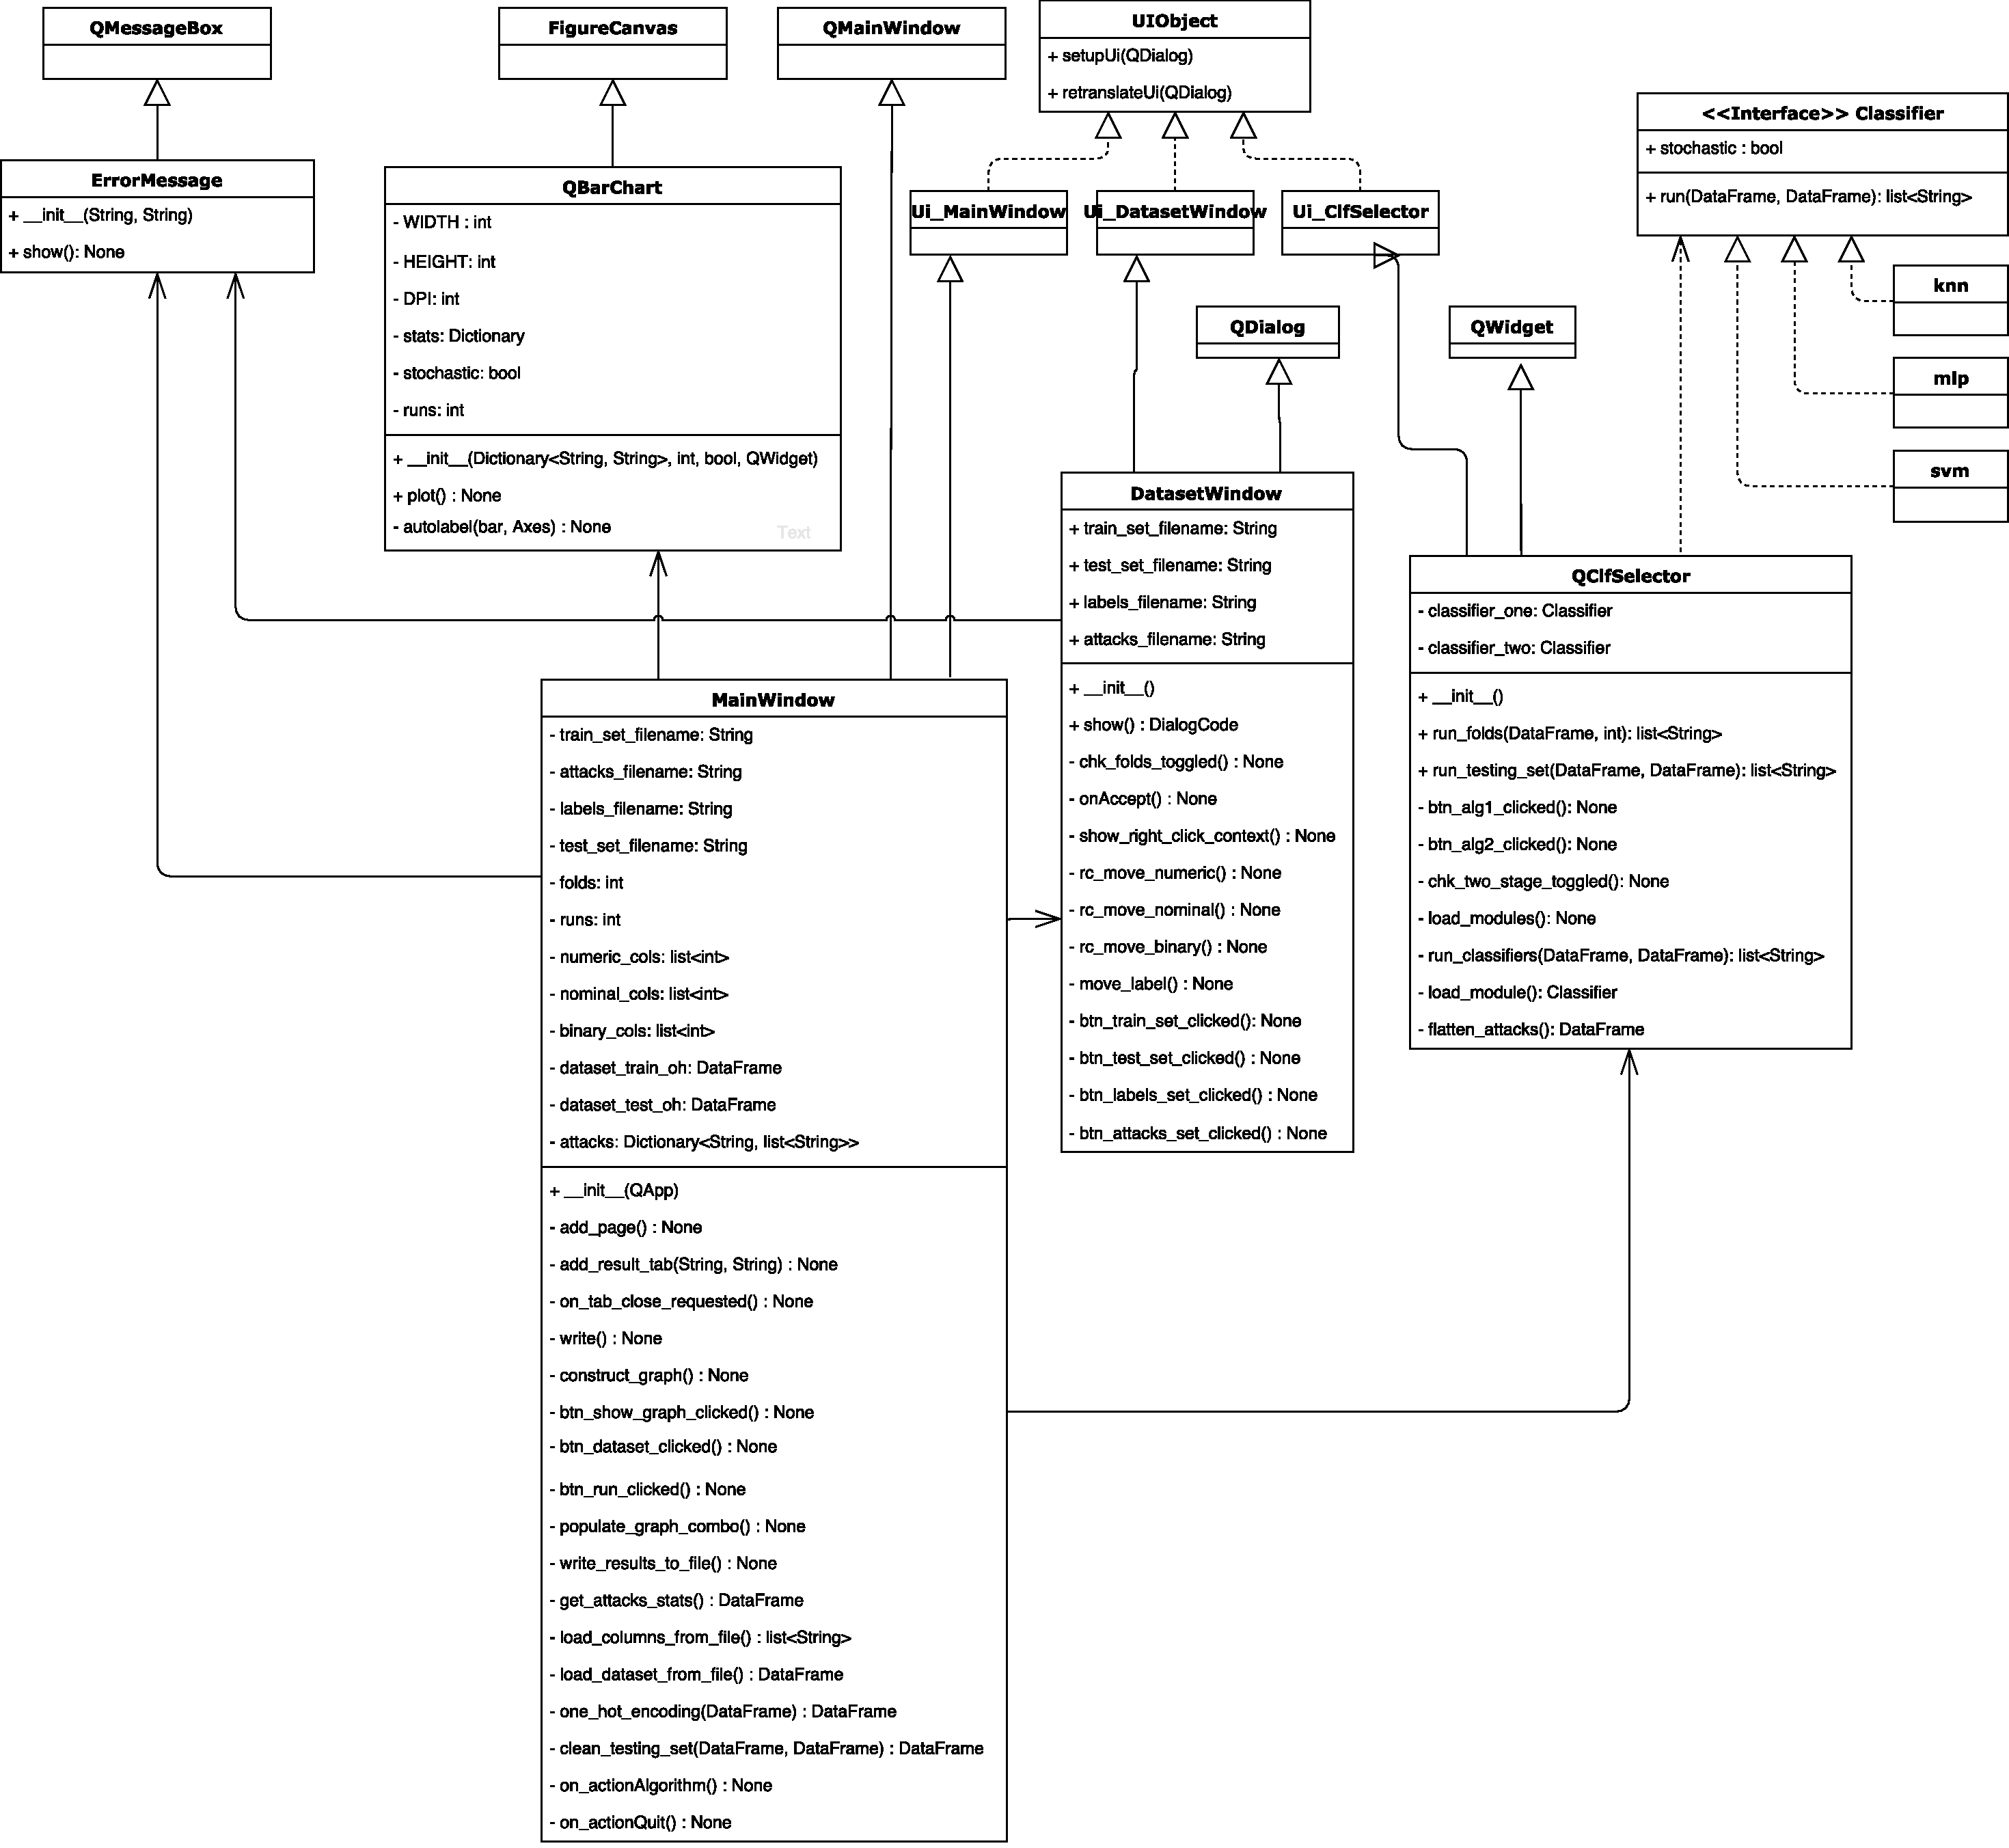
\includegraphics[width=1.2\textwidth, center]{figures/classuml.pdf}}
\caption{UML Class Diagram}
\end{figure}

\newpage

\section{Use Case Diagram} \label{usecase}
\begin{figure}[H]
	\makebox[\textwidth][c]{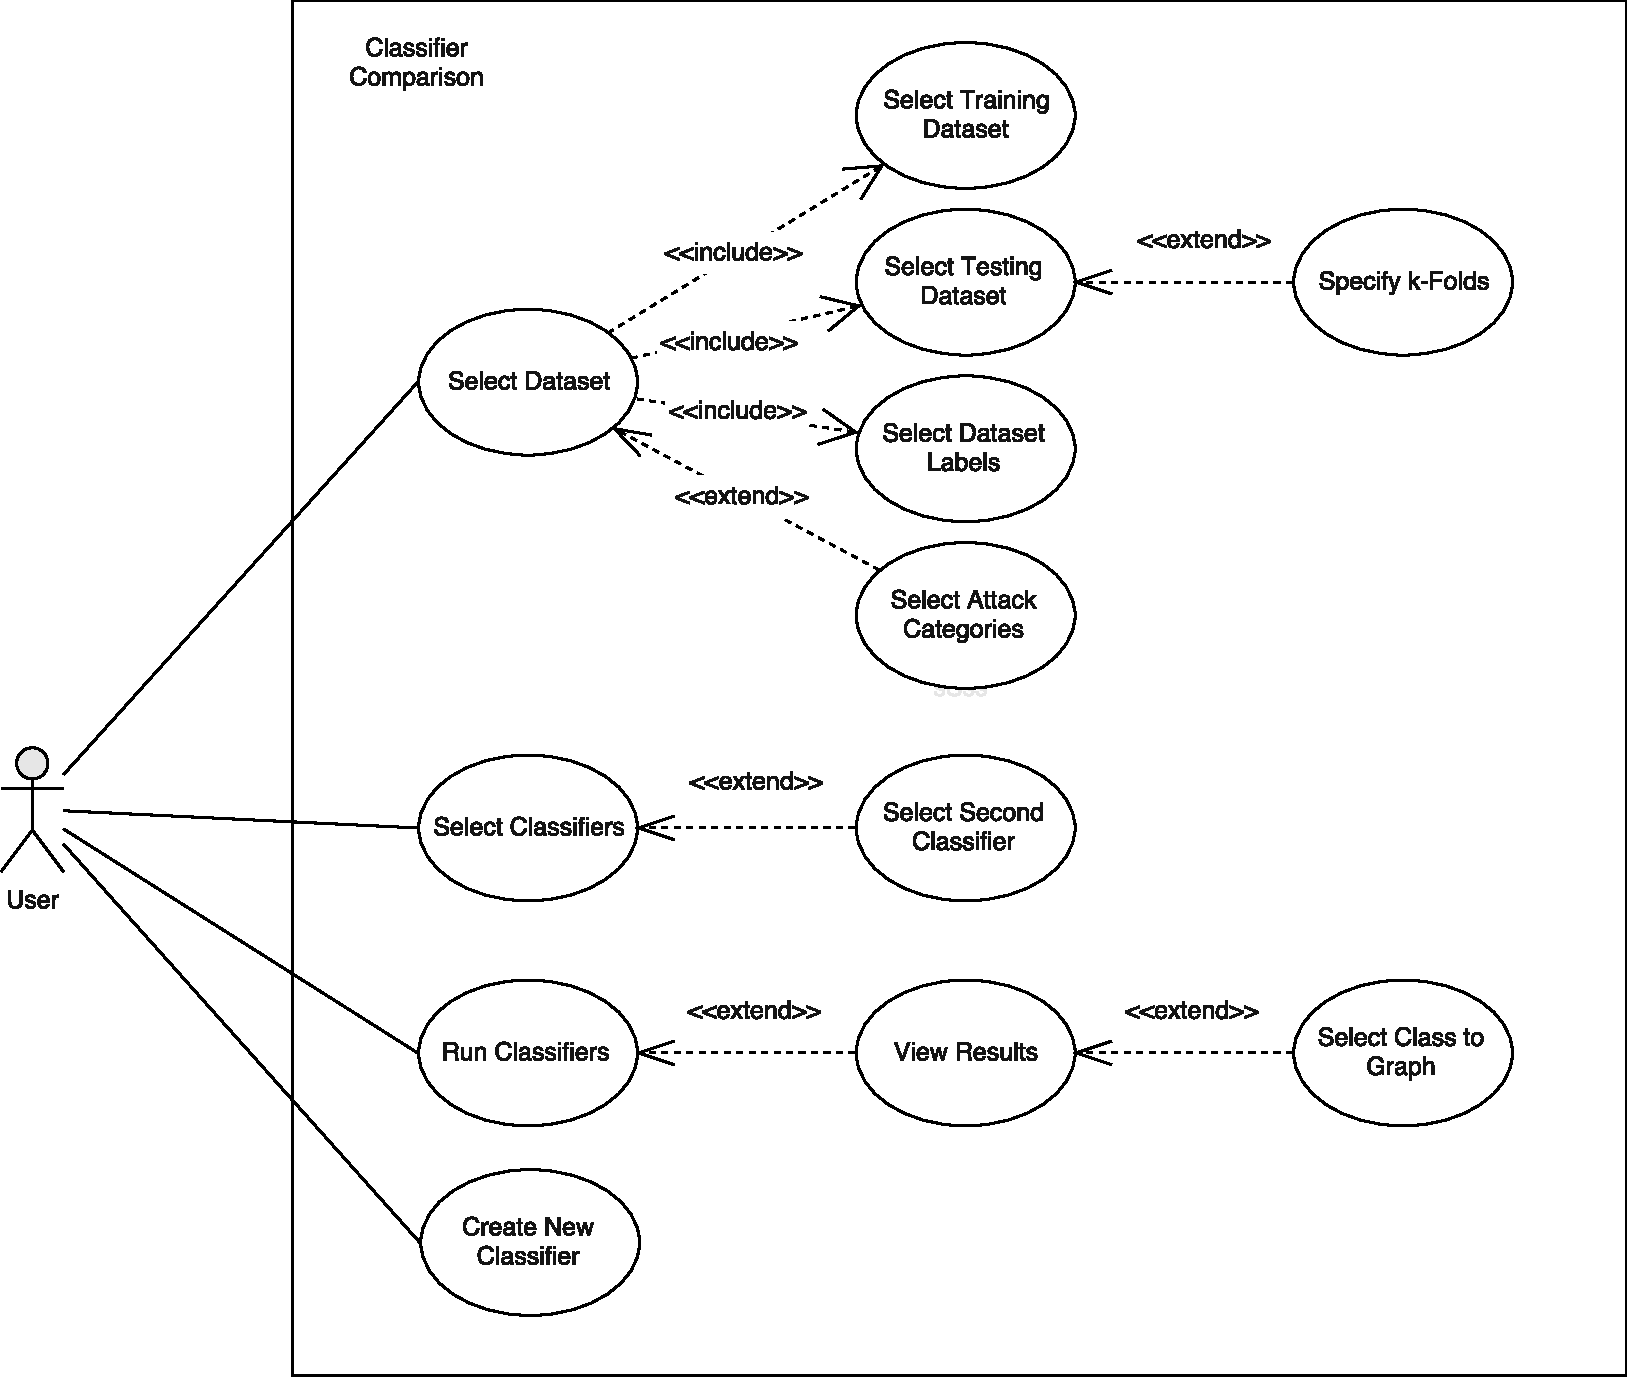
\includegraphics[width=1.2\textwidth, center]{figures/usecase.pdf}}
\caption{UML Use Case Diagram}
\end{figure}

\newpage

\section{NSL-KDD Features} \label{kddfeatures}
\begin{longtable}{@{}ll@{}}
\caption{NSL-KDD Features} \\
\label{nf} \\
\toprule
Feature & Type \\ \midrule
duration & continuous \\
protocol\_type & symbolic \\
service & symbolic \\
flag & symbolic \\
src\_bytes & continuous \\
dst\_bytes & continuous \\
land & binary \\
wrong\_fragment & continuous \\
urgent & continuous \\
hot & continuous \\
num\_failed\_logins & continuous \\
logged\_in & binary \\
num\_compromised & continuous \\
root\_shell & binary \\
su\_attempted & binary \\
num\_root & continuous \\
num\_file\_creations & continuous \\
num\_shells & continuous \\
num\_access\_files & continuous \\
num\_outbound\_cmds & continuous \\
is\_host\_login & binary \\
is\_guest\_login & binary \\
count & continuous \\
srv\_count & continuous \\
serror\_rate & continuous \\
srv\_serror\_rate & continuous \\
rerror\_rate & continuous \\
srv\_rerror\_rate & continuous \\
same\_srv\_rate & continuous \\
diff\_srv\_rate & continuous \\
srv\_diff\_host\_rate & continuous \\
dst\_host\_count & continuous \\
dst\_host\_srv\_count & continuous \\
dst\_host\_same\_srv\_rate & continuous \\
dst\_host\_diff\_srv\_rate & continuous \\
dst\_host\_same\_src\_port\_rate & continuous \\
dst\_host\_srv\_diff\_host\_rate & continuous \\
dst\_host\_serror\_rate & continuous \\
dst\_host\_srv\_serror\_rate & continuous \\
dst\_host\_rerror\_rate & continuous \\
dst\_host\_srv\_rerror\_rate & continuous \\
\bottomrule
\end{longtable}


\newpage

\section{UNSW-NB15 Features} \label{unswfeatures}

% Please add the following required packages to your document preamble:
% \usepackage{booktabs}
\begin{longtable}{@{}p{0.22\textwidth}p{0.1\textwidth}p{0.63\textwidth}@{}}
\caption{UNSW-NB15 Fields}\\
\label{unswfieldstable}\\
\toprule
Field & Type & Description \\ \midrule
dur & Float & Record total duration \\
proto & nominal & Transaction protocol \\
service & nominal & http, ftp, smtp, ssh, dns, ftp-data ,irc  and (-) if not much used service \\
state & nominal & Indicates to the state and its dependent protocol, e.g. ACC, CLO, CON, ECO, ECR, FIN, INT, MAS, PAR, REQ, RST, TST, TXD, URH, URN, and (-) (if not used state) \\
spkts & integer & Source to destination packet count \\
dpkts & integer & Destination to source packet count \\
sbytes & Integer & Source to destination transaction bytes \\
dbytes & Integer & Destination to source transaction bytes \\
rate & Float & Connection rate \\
sttl & Integer & Source to destination time to live value \\
dttl & Integer & Destination to source time to live value \\
sload & Float & Source bits per second \\
dload & Float & Destination bits per second \\
sloss & Integer & Source packets retransmitted or dropped \\
dloss & Integer & Destination packets retransmitted or dropped \\
Sintpkt & Float & Source interpacket arrival time (mSec) \\
Dintpkt & Float & Destination interpacket arrival time (mSec) \\
sjit & Float & Source jitter (mSec) \\
djit & Float & Destination jitter (mSec) \\
swin & integer & Source TCP window advertisement value \\
stcpb & integer & Source TCP base sequence number \\
dtcpb & integer & Destination TCP base sequence number \\
dwin & integer & Destination TCP window advertisement value \\
tcprtt & Float & TCP connection setup round-trip time, the sum of �synack� and �ackdat�. \\
synack & Float & TCP connection setup time, the time between the SYN and the SYN\_ACK packets. \\
ackdat & Float & TCP connection setup time, the time between the SYN\_ACK and the ACK packets. \\
smean & integer & Mean of the ?ow packet size transmitted by the src \\
dmean & integer & Mean of the ?ow packet size transmitted by the dst \\
trans\_depth & integer & Represents the pipelined depth into the connection of http request/response transaction \\
res\_bdy\_len & integer & Actual uncompressed content size of the data transferred from the server�s http service. \\
ct\_srv\_src & integer & No. of connections that contain the same service (14) and source address (1) in 100 connections according to the last time (26). \\
ct\_state\_ttl & Integer & No. for each state (6) according to specific range of values for source/destination time to live (10) (11). \\
ct\_dst\_ltm & integer & No. of connections of the same destination address (3) in 100 connections according to the last time (26). \\
ct\_src\_dport\_ltm & integer & No of connections of the same source address (1) and the destination port (4) in 100 connections according to the last time (26). \\
ct\_dst\_sport\_ltm & integer & No of connections of the same destination address (3) and the source port (2) in 100 connections according to the last time (26). \\
ct\_dst\_src\_ltm & integer & No of connections of the same source (1) and the destination (3) address in in 100 connections according to the last time (26). \\
is\_ftp\_login & binary & If the ftp session is accessed by user and password then 1 else 0. \\
ct\_ftp\_cmd & integer & No of flows that has a command in ftp session. \\
ct\_flw\_http\_mthd & Integer & No. of flows that has methods such as Get and Post in http service. \\
ct\_src\_ltm & integer & No. of connections of the same source address (1) in 100 connections according to the last time (26). \\
ct\_srv\_dst & integer & No. of connections that contain the same service (14) and destination address (3) in 100 connections according to the last time (26). \\
is\_sm\_ips\_ports & binary & If source (1) and destination (3)IP addresses equal and port numbers (2)(4)  equal then, this variable takes value 1 else 0 \\
attack\_cat & nominal & The name of each attack category. In this data set , nine categories e.g. Fuzzers, Analysis, Backdoors, DoS Exploits, Generic, Reconnaissance, Shellcode and Worms \\
labels & binary & 0 for normal and 1 for attack records \\ \bottomrule
\end{longtable}


\newpage

\section{NSL-KDD Precision}
% Please add the following required packages to your document preamble:
% \usepackage{booktabs}
\begin{table}[H]
\centering
\caption{NSL-KDD Classifiers Precision Table}
\label{nslprecisiontable}
\begin{tabular}{@{}llllll@{}}
\toprule
 & dos & u2r & r2l & probe & normal \\ \midrule
K-NN & 0.91 & 0.17 & 0.69 & 0.9 & 0.99 \\
MLP & 0.94 & 0.38 & 0.79 & 0.98 & 0.99 \\
SVM & 0.93 & 0.64 & 0.83 & 0.99 & 0.99 \\
K-NN/K-NN & 0.9 & 0.18 & 0.73 & 0.91 & 0.99 \\
K-NN/MLP & 0.94 & 0.3 & 0.51 & 0.98 & 0.99 \\
K-NN/SVM & 0.93 & 0.58 & 0.64 & 0.96 & 0.99 \\
MLP/K-NN & 0.89 & 0.33 & 0.51 & 0.91 & 0.99 \\
MLP/MLP & 0.94 & 0.49 & 0.71 & 0.98 & 0.99 \\
MLP/SVM & 0.93 & 0.73 & 0.8 & 0.97 & 0.99 \\
SVM/K-NN & 0.9 & 0.21 & 0.44 & 0.91 & 0.99 \\
SVM/MLP & 0.94 & 0.37 & 0.49 & 0.98 & 0.99 \\
SVM/SVM & 0.93 & 0.65 & 0.83 & 0.96 & 0.99 \\ \bottomrule
\end{tabular}
\end{table}

\begin{figure}[H]
\begin{adjustbox}{height=0.68\paperheight, center=\textwidth}
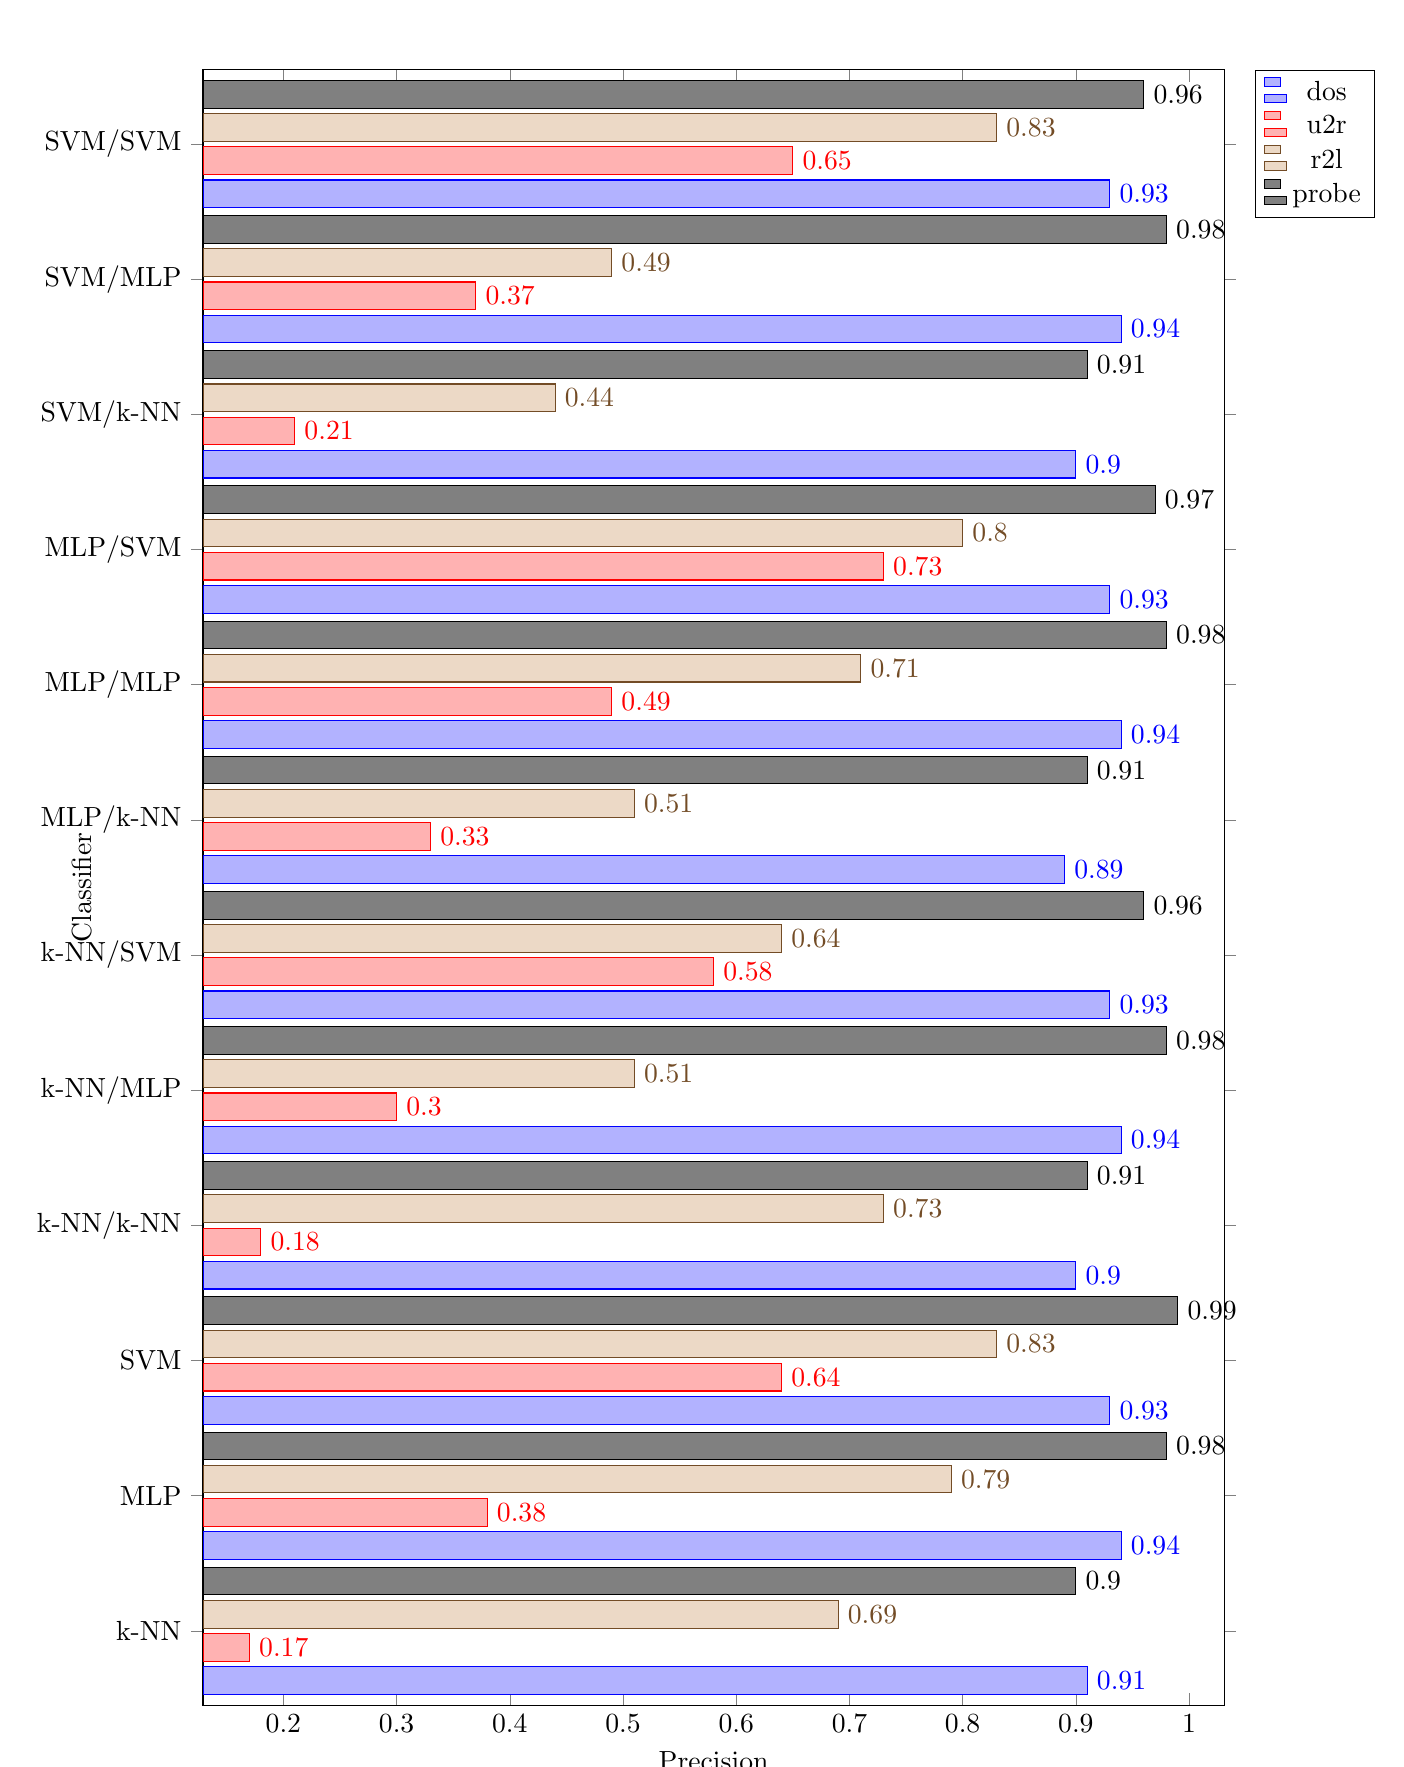
\begin{tikzpicture}
\begin{axis}[
    xbar,
    enlargelimits=0.05,
    legend pos=outer north east,
    ylabel={Classifier},
    xlabel={Precision},
    y label style={at={(axis description cs:-0.1,.5)},anchor=south},
    symbolic y coords={k-NN,MLP,SVM,k-NN/k-NN,k-NN/MLP,k-NN/SVM,MLP/k-NN,MLP/MLP,MLP/SVM,SVM/k-NN,SVM/MLP,SVM/SVM},
    ytick=data,
    nodes near coords,
    nodes near coords align={horizontal},
    width=1.2\textwidth,
    height=0.8\paperheight
    ]
    \addplot coordinates {(0.91,k-NN) (0.94,MLP) (0.93,SVM) 
	                  (0.90,k-NN/k-NN) (0.94,k-NN/MLP) (0.93,k-NN/SVM) 
		          (0.89,MLP/k-NN) (0.94,MLP/MLP) (0.93,MLP/SVM) 
		          (0.90,SVM/k-NN) (0.94,SVM/MLP) (0.93,SVM/SVM)};
    \addplot coordinates {(0.17,k-NN) (0.38,MLP) (0.64,SVM) 
	                  (0.18,k-NN/k-NN) (0.30,k-NN/MLP) (0.58,k-NN/SVM) 
		          (0.33,MLP/k-NN) (0.49,MLP/MLP) (0.73,MLP/SVM) 
		          (0.21,SVM/k-NN) (0.37,SVM/MLP) (0.65,SVM/SVM)};
    \addplot coordinates {(0.69,k-NN) (0.79,MLP) (0.83,SVM) 
	                  (0.73,k-NN/k-NN) (0.51,k-NN/MLP) (0.64,k-NN/SVM) 
		          (0.51,MLP/k-NN) (0.71,MLP/MLP) (0.80,MLP/SVM) 
		          (0.44,SVM/k-NN) (0.49,SVM/MLP) (0.83,SVM/SVM)};
    \addplot coordinates {(0.90,k-NN) (0.98,MLP) (0.99,SVM) 
	                  (0.91,k-NN/k-NN) (0.98,k-NN/MLP) (0.96,k-NN/SVM) 
		          (0.91,MLP/k-NN) (0.98,MLP/MLP) (0.97,MLP/SVM) 
		          (0.91,SVM/k-NN) (0.98,SVM/MLP) (0.96,SVM/SVM)};
        \legend{dos,u2r,r2l,probe}
\end{axis}
\end{tikzpicture}
\end{adjustbox}
\caption{Classifiers Precision Graph}
\end{figure}


\newpage


\section{NSL-KDD Recall}
% Please add the following required packages to your document preamble:
% \usepackage{booktabs}
\begin{table}[H]
\centering
\caption{NSL-KDD Classifiers Recall Table}
\label{nslrecalltable}
\begin{tabular}{@{}llllll@{}}
\toprule
          & dos  & u2r  & r2l  & probe & normal \\ \midrule
K-NN      & 0.96 & 0.19 & 0.62 & 0.86  & 0.99   \\
K-NN/K-NN & 0.97 & 0.31 & 0.62 & 0.87  & 0.99   \\
K-NN/MLP  & 0.94 & 0.19 & 0.57 & 0.98  & 0.99   \\
K-NN/SVM  & 0.9  & 0.21 & 0.55 & 0.97  & 0.99   \\
MLP       & 0.95 & 0.34 & 0.57 & 0.98  & 0.99   \\
MLP/K-NN  & 0.89 & 0.28 & 0.53 & 0.88  & 0.99   \\
MLP/MLP   & 0.94 & 0.44 & 0.65 & 0.98  & 0.99   \\
MLP/SVM   & 0.92 & 0.34 & 0.61 & 0.97  & 0.99   \\
SVM       & 0.93 & 0.36 & 0.6  & 0.95  & 0.99   \\
SVM/K-NN  & 0.93 & 0.29 & 0.56 & 0.88  & 0.99   \\
SVM/MLP   & 0.98 & 0.51 & 0.57 & 0.98  & 0.99   \\
SVM/SVM   & 0.93 & 0.36 & 0.6  & 0.97  & 0.99   \\ \bottomrule
\end{tabular}
\end{table}

\begin{figure}[H]
\begin{adjustbox}{width=\textwidth, center=\textwidth}
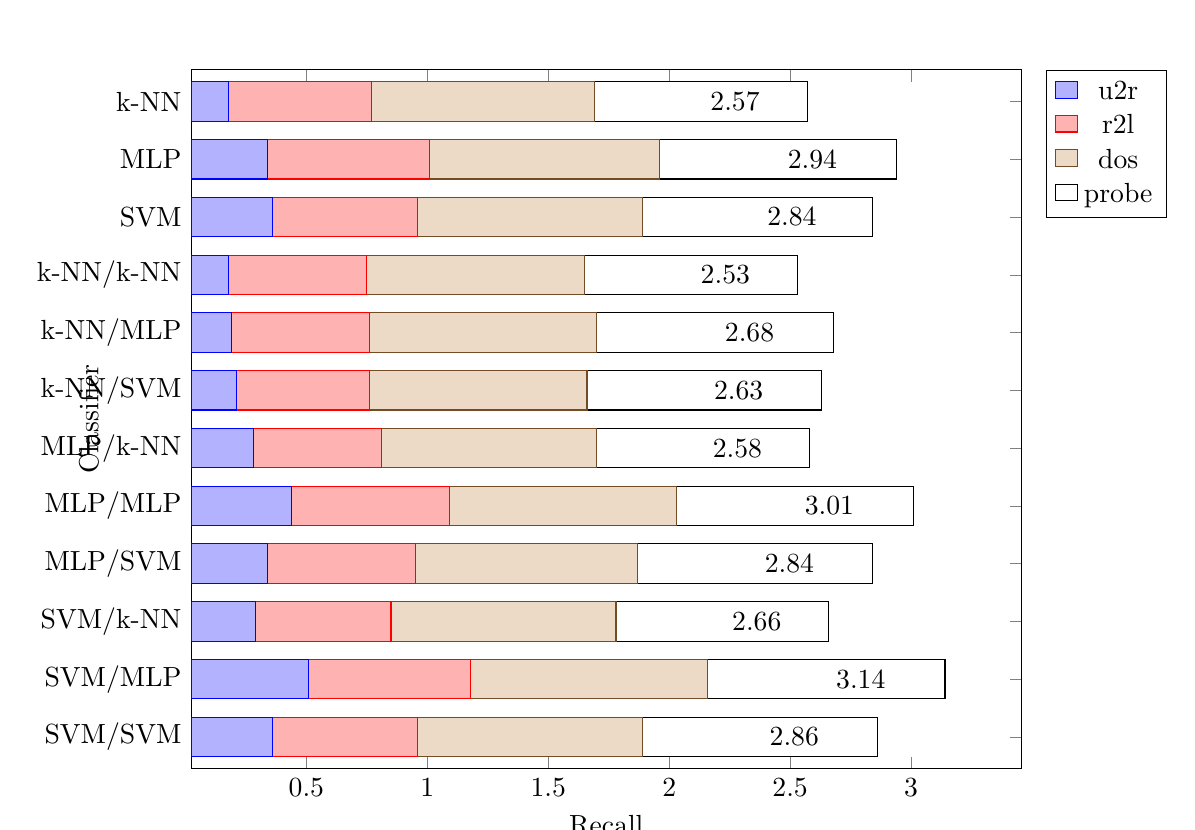
\begin{tikzpicture}
\begin{axis}[
    xbar stacked,
    enlargelimits=0.05,
    legend pos=outer north east,
    ylabel={Classifier},
    xlabel={Recall},
    y label style={at={(axis description cs:-0.1,.5)},anchor=south},
    symbolic y coords={k-NN,MLP,SVM,k-NN/k-NN,k-NN/MLP,k-NN/SVM,MLP/k-NN,MLP/MLP,MLP/SVM,SVM/k-NN,SVM/MLP,SVM/SVM},
    ytick=data,
    %nodes near coords,
    %nodes near coords align={horizontal},
    bar width = 0.5cm,
    xmax = 3.3,
    y dir = reverse,
    width=1.0\textwidth,
    ]
    \addplot coordinates {(0.18,k-NN) (0.34,MLP) (0.36,SVM) 
	                  (0.18,k-NN/k-NN) (0.19,k-NN/MLP) (0.21,k-NN/SVM) 
		          (0.28,MLP/k-NN) (0.44,MLP/MLP) (0.34,MLP/SVM) 
		          (0.29,SVM/k-NN) (0.51,SVM/MLP) (0.36,SVM/SVM)};
    \addplot coordinates {(0.59,k-NN) (0.67,MLP) (0.60,SVM) 
	                  (0.57,k-NN/k-NN) (0.57,k-NN/MLP) (0.55,k-NN/SVM) 
		          (0.53,MLP/k-NN) (0.65,MLP/MLP) (0.61,MLP/SVM) 
		          (0.56,SVM/k-NN) (0.67,SVM/MLP) (0.60,SVM/SVM)};
    \addplot coordinates {(0.92,k-NN) (0.95,MLP) (0.93,SVM) 
	                  (0.90,k-NN/k-NN) (0.94,k-NN/MLP) (0.90,k-NN/SVM) 
		          (0.89,MLP/k-NN) (0.94,MLP/MLP) (0.92,MLP/SVM) 
		          (0.93,SVM/k-NN) (0.98,SVM/MLP) (0.93,SVM/SVM)};

    \addplot [point meta = x, nodes near coords, nodes near coords align={anchor=west}] coordinates {(0.88,k-NN) (0.98,MLP) (0.95,SVM) 
	                  (0.88,k-NN/k-NN) (0.98,k-NN/MLP) (0.97,k-NN/SVM) 
		          (0.88,MLP/k-NN) (0.98,MLP/MLP) (0.97,MLP/SVM) 
		          (0.88,SVM/k-NN) (0.98,SVM/MLP) (0.97,SVM/SVM)};
    \legend{u2r,r2l,dos,probe}
\end{axis}
\end{tikzpicture}
\end{adjustbox}
\caption{Classifiers Recall Graph}
\end{figure}


\newpage

\section{NSL-KDD F1-Score}
% Please add the following required packages to your document preamble:
% \usepackage{booktabs}
\begin{table}[H]
\centering
\caption{NSL-KDD Classifiers f1-Score Table}
\label{nslf1scoretable}
\begin{tabular}{@{}llllll@{}}
\toprule
          & dos  & u2r  & r2l  & probe & normal \\ \midrule
K-NN      & 0.93 & 0.16 & 0.65 & 0.88  & 0.99   \\
K-NN/K-NN & 0.93 & 0.28 & 0.62 & 0.88  & 0.99   \\
K-NN/MLP  & 0.94 & 0.23 & 0.54 & 0.98  & 0.99   \\
K-NN/SVM  & 0.91 & 0.29 & 0.58 & 0.96  & 0.99   \\
MLP       & 0.95 & 0.36 & 0.72 & 0.98  & 0.99   \\
MLP/K-NN  & 0.89 & 0.24 & 0.51 & 0.89  & 0.99   \\
MLP/MLP   & 0.94 & 0.46 & 0.67 & 0.98  & 0.99   \\
MLP/SVM   & 0.93 & 0.45 & 0.68 & 0.97  & 0.99   \\
SVM       & 0.93 & 0.45 & 0.69 & 0.97  & 0.99   \\
SVM/K-NN  & 0.91 & 0.22 & 0.48 & 0.89  & 0.99   \\
SVM/MLP   & 0.96 & 0.43 & 0.54 & 0.98  & 0.99   \\
SVM/SVM   & 0.93 & 0.45 & 0.69 & 0.96  & 0.99   \\ \bottomrule
\end{tabular}
\end{table}

\begin{figure}[H]
\begin{adjustbox}{height=0.64\paperheight, center=\textwidth}
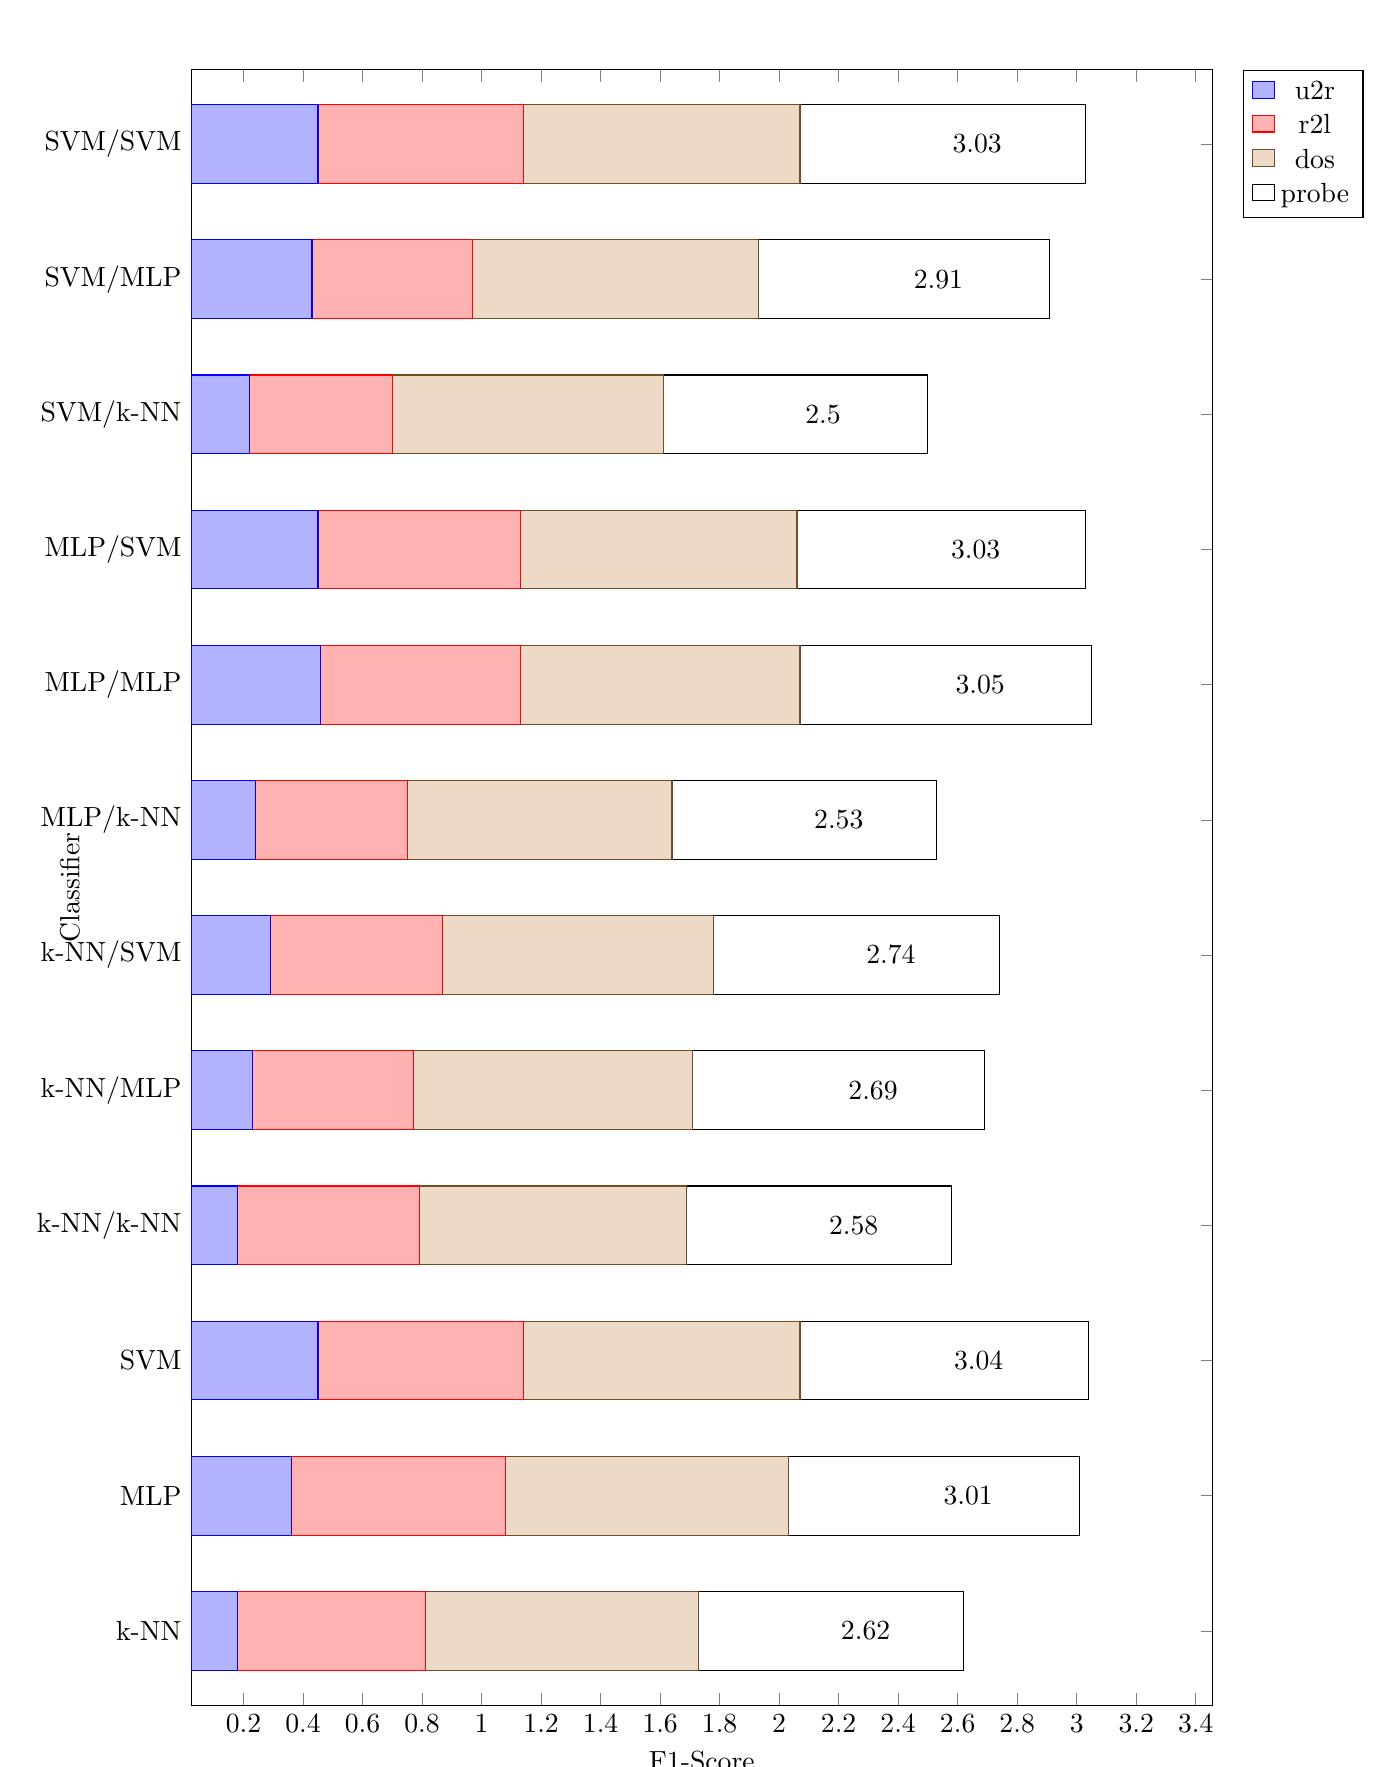
\begin{tikzpicture}
\begin{axis}[
    xbar stacked,
    enlargelimits=0.05,
    legend pos=outer north east,
    ylabel={Classifier},
    xlabel={F1-Score},
    y label style={at={(axis description cs:-0.1,.5)},anchor=south},
    symbolic y coords={k-NN,MLP,SVM,k-NN/k-NN,k-NN/MLP,k-NN/SVM,MLP/k-NN,MLP/MLP,MLP/SVM,SVM/k-NN,SVM/MLP,SVM/SVM},
    ytick=data,
    %nodes near coords,
    %nodes near coords align={horizontal},
    bar width = 1cm,
    xmax=3.3,
    width=1.2\textwidth,
    height=0.8\paperheight
    ]
    \addplot coordinates {(0.18,k-NN) (0.36,MLP) (0.45,SVM) 
	                  (0.18,k-NN/k-NN) (0.23,k-NN/MLP) (0.29,k-NN/SVM) 
		          (0.24,MLP/k-NN) (0.46,MLP/MLP) (0.45,MLP/SVM) 
		          (0.22,SVM/k-NN) (0.43,SVM/MLP) (0.45,SVM/SVM)};
    \addplot coordinates {(0.63,k-NN) (0.72,MLP) (0.69,SVM) 
	                  (0.61,k-NN/k-NN) (0.54,k-NN/MLP) (0.58,k-NN/SVM) 
		          (0.51,MLP/k-NN) (0.67,MLP/MLP) (0.68,MLP/SVM) 
		          (0.48,SVM/k-NN) (0.54,SVM/MLP) (0.69,SVM/SVM)};
    \addplot coordinates {(0.92,k-NN) (0.95,MLP) (0.93,SVM) 
	                  (0.90,k-NN/k-NN) (0.94,k-NN/MLP) (0.91,k-NN/SVM) 
		          (0.89,MLP/k-NN) (0.94,MLP/MLP) (0.93,MLP/SVM) 
		          (0.91,SVM/k-NN) (0.96,SVM/MLP) (0.93,SVM/SVM)};

    \addplot [point meta = x, nodes near coords, nodes near coords align={anchor=west}] coordinates {(0.89,k-NN) (0.98,MLP) (0.97,SVM) 
	                  (0.89,k-NN/k-NN) (0.98,k-NN/MLP) (0.96,k-NN/SVM) 
		          (0.89,MLP/k-NN) (0.98,MLP/MLP) (0.97,MLP/SVM) 
		          (0.89,SVM/k-NN) (0.98,SVM/MLP) (0.96,SVM/SVM)};
        \legend{u2r,r2l,dos,probe}
\end{axis}
\end{tikzpicture}
\end{adjustbox}
\caption{Classifiers f1-Score Graph}
\end{figure}


\newpage


\section{UNSW-NB15 Precision}
% Please add the following required packages to your document preamble:
% \usepackage{booktabs}
\begin{table}[H]
\centering
\caption{UNSW-NB15 Classifiers Precision Table}
\label{unswprecisiontable}
\begin{tabular}{@{}lllllllllll@{}}
\toprule
 & \rotatebox{90}{Analysis} & \rotatebox{90}{Backdoor} & \rotatebox{90}{DoS} & \rotatebox{90}{Exploits} & \rotatebox{90}{Fuzzers} & \rotatebox{90}{Generic} & \rotatebox{90}{Recon} & \rotatebox{90}{Shellcode} & \rotatebox{90}{Worms} & \rotatebox{90}{Normal} \\ \midrule
K-NN & 0.1 & 0.08 & 0.22 & 0.23 & 0.19 & 0.95 & 0.7 & 0.18 & 0 & 0.73 \\
MLP & 0.13 & 0.13 & 0.38 & 0.62 & 0.57 & 0.98 & 0.71 & 0.3 & 0.49 & 0.93 \\
SVM & 0.06 & 0 & 0.23 & 0.59 & 0.6 & 0.99 & 0.69 & 0.44 & 0.1 & 0.9 \\
K-NN/K-NN & 0.1 & 0.06 & 0.19 & 0.24 & 0.19 & 0.95 & 0.62 & 0.14 & 0 & 0.73 \\
K-NN/MLP & 0.01 & 0.13 & 0.34 & 0.4 & 0.25 & 0.99 & 0.6 & 0.16 & 0.27 & 0.73 \\
K-NN/SVM & 0.01 & 0 & 0.17 & 0.39 & 0.24 & 0.99 & 0.64 & 0.31 & 0 & 0.73 \\
MLP/K-NN & 0.1 & 0.06 & 0.21 & 0.46 & 0.25 & 0.95 & 0.63 & 0.16 & 0 & 0.94 \\
MLP/MLP & 0.11 & 0.13 & 0.38 & 0.61 & 0.52 & 0.98 & 0.68 & 0.32 & 0.53 & 0.94 \\
MLP/SVM & 0.06 & 0 & 0.23 & 0.58 & 0.59 & 0.98 & 0.68 & 0.44 & 1 & 0.93 \\
SVM/K-NN & 0.1 & 0.06 & 0.21 & 0.45 & 0.22 & 0.95 & 0.63 & 0.15 & 0 & 0.92 \\
SVM/MLP & 0.11 & 0.14 & 0.38 & 0.61 & 0.47 & 0.98 & 0.65 & 0.28 & 0.53 & 0.92 \\
SVM/SVM & 0.06 & 0 & 0.23 & 0.57 & 0.53 & 0.98 & 0.66 & 0.39 & 1 & 0.92 \\ \bottomrule
\end{tabular}
\end{table}

\begin{figure}[H]
\begin{adjustbox}{width=1.0\textwidth, center=\textwidth}
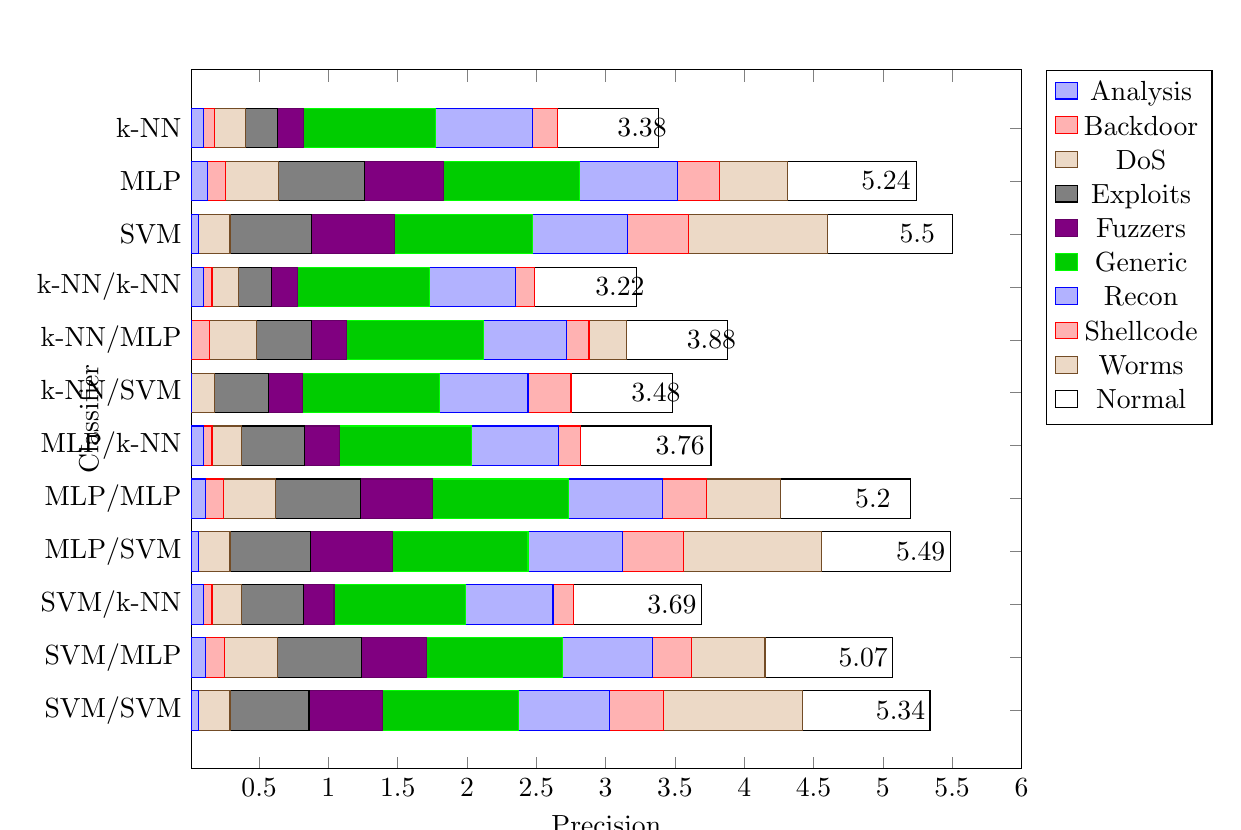
\begin{tikzpicture}
\begin{axis}[
    xbar stacked,
    enlarge x limits=0.00,
    legend pos=outer north east,
    ylabel={Classifier},
    xlabel={Precision},
    y label style={at={(axis description cs:-0.1,.5)},anchor=south},
    symbolic y coords={k-NN,MLP,SVM,k-NN/k-NN,k-NN/MLP,k-NN/SVM,MLP/k-NN,MLP/MLP,MLP/SVM,SVM/k-NN,SVM/MLP,SVM/SVM},
    ytick=data,
    %nodes near coords,
    %nodes near coords align={horizontal},
    point meta=rawx,
    bar width = 0.5cm,
    y dir = reverse,
    xmax = 6,
    width=1.0\textwidth,
    ]
    % Analysis
    \addplot coordinates {(0.10,k-NN) (0.13,MLP) (0.06,SVM) 
	                  (0.10,k-NN/k-NN) (0.01,k-NN/MLP) (0.01,k-NN/SVM) 
		          (0.10,MLP/k-NN) (0.11,MLP/MLP) (0.06,MLP/SVM) 
		          (0.10,SVM/k-NN) (0.11,SVM/MLP) (0.06,SVM/SVM)};
    % Backdoor
    \addplot coordinates {(0.08,k-NN) (0.13,MLP) (0.00,SVM) 
	                  (0.06,k-NN/k-NN) (0.13,k-NN/MLP) (0.00,k-NN/SVM) 
		          (0.06,MLP/k-NN) (0.13,MLP/MLP) (0.00,MLP/SVM) 
		          (0.06,SVM/k-NN) (0.14,SVM/MLP) (0.00,SVM/SVM)};
    % DoS
    \addplot  coordinates {(0.22,k-NN) (0.38,MLP) (0.23,SVM) 
	                  (0.19,k-NN/k-NN) (0.34,k-NN/MLP) (0.17,k-NN/SVM) 
		          (0.21,MLP/k-NN) (0.38,MLP/MLP) (0.23,MLP/SVM) 
		          (0.21,SVM/k-NN) (0.38,SVM/MLP) (0.23,SVM/SVM)};
    % Exploits
    \addplot  coordinates {(0.23,k-NN) (0.62,MLP) (0.59,SVM) 
	                  (0.24,k-NN/k-NN) (0.40,k-NN/MLP) (0.39,k-NN/SVM) 
		          (0.46,MLP/k-NN) (0.61,MLP/MLP) (0.58,MLP/SVM) 
		          (0.45,SVM/k-NN) (0.61,SVM/MLP) (0.57,SVM/SVM)};
    % Fuzzers
    \addplot  coordinates {(0.19,k-NN) (0.57,MLP) (0.60,SVM) 
	                  (0.19,k-NN/k-NN) (0.25,k-NN/MLP) (0.24,k-NN/SVM) 
		          (0.25,MLP/k-NN) (0.52,MLP/MLP) (0.59,MLP/SVM) 
		          (0.22,SVM/k-NN) (0.47,SVM/MLP) (0.53,SVM/SVM)};
    % Generic
    \addplot coordinates {(0.95,k-NN) (0.98,MLP) (0.99,SVM) 
	                  (0.95,k-NN/k-NN) (0.99,k-NN/MLP) (0.99,k-NN/SVM) 
		          (0.95,MLP/k-NN) (0.98,MLP/MLP) (0.98,MLP/SVM) 
		          (0.95,SVM/k-NN) (0.98,SVM/MLP) (0.98,SVM/SVM)};
    % Reconnaissance
    \addplot coordinates {(0.70,k-NN) (0.71,MLP) (0.69,SVM) 
	                  (0.62,k-NN/k-NN) (0.60,k-NN/MLP) (0.64,k-NN/SVM) 
		          (0.63,MLP/k-NN) (0.68,MLP/MLP) (0.68,MLP/SVM) 
		          (0.63,SVM/k-NN) (0.65,SVM/MLP) (0.66,SVM/SVM)};
    % Shellcode
    \addplot coordinates {(0.18,k-NN) (0.30,MLP) (0.44,SVM) 
	                  (0.14,k-NN/k-NN) (0.16,k-NN/MLP) (0.31,k-NN/SVM) 
		          (0.16,MLP/k-NN) (0.32,MLP/MLP) (0.44,MLP/SVM) 
		          (0.15,SVM/k-NN) (0.28,SVM/MLP) (0.39,SVM/SVM)};
    % Worms
    \addplot coordinates {(0.00,k-NN) (0.49,MLP) (1.00,SVM) 
	                  (0.00,k-NN/k-NN) (0.27,k-NN/MLP) (0.00,k-NN/SVM) 
		          (0.00,MLP/k-NN) (0.53,MLP/MLP) (1.00,MLP/SVM) 
		          (0.00,SVM/k-NN) (0.53,SVM/MLP) (1.00,SVM/SVM)};
    % Normal
    \addplot [point meta = x, nodes near coords, nodes near coords align={anchor=west}] coordinates {(0.73,k-NN) (0.93,MLP) (0.90,SVM) 
	                  (0.73,k-NN/k-NN) (0.73,k-NN/MLP) (0.73,k-NN/SVM) 
		          (0.94,MLP/k-NN) (0.94,MLP/MLP) (0.93,MLP/SVM) 
		          (0.92,SVM/k-NN) (0.92,SVM/MLP) (0.92,SVM/SVM)};


        \legend{Analysis, Backdoor, DoS, Exploits, Fuzzers, Generic, Recon, Shellcode, Worms, Normal}
\end{axis}
\end{tikzpicture}
\end{adjustbox}
\caption{UNSW-NB15 Classifiers Precision Graph}
\label{unswprecision}
\end{figure}


\newpage

\section{UNSW-NB15 Recall}
% Please add the following required packages to your document preamble:
% \usepackage{booktabs}
\begin{table}[H]
\centering
\caption{UNSW-NB15 Classifier Recall Table}
\label{unswrecalltable}
\begin{tabular}{@{}lllllllllll@{}}
\toprule
 & \rotatebox{90}{Analysis} & \rotatebox{90}{Backdoor} & \rotatebox{90}{DoS} & \rotatebox{90}{Exploits} & \rotatebox{90}{Fuzzers} & \rotatebox{90}{Generic} & \rotatebox{90}{Recon} & \rotatebox{90}{Shellcode} & \rotatebox{90}{Worms} & \rotatebox{90}{Normal} \\ \midrule
k-NN & 0.33 & 0.08 & 0.24 & 0.26 & 0.14 & 0.96 & 0.36 & 0.03 & 0 & 0.72 \\
MLP & 0.01 & 0.02 & 0.15 & 0.78 & 0.6 & 0.97 & 0.69 & 0.21 & 0.09 & 0.95 \\
SVM & 0 & 0 & 0.13 & 0.82 & 0.43 & 0.96 & 0.6 & 0.23 & 0.05 & 0.92 \\
k-NN/k-NN & 0.35 & 0.08 & 0.19 & 0.26 & 0.14 & 0.96 & 0.37 & 0.03 & 0 & 0.72 \\
k-NN/MLP & 0.01 & 0.03 & 0.13 & 0.43 & 0.4 & 0.96 & 0.52 & 0.14 & 0.03 & 0.72 \\
k-NN/SVM & 0 & 0 & 0.11 & 0.48 & 0.3 & 0.96 & 0.51 & 0.13 & 0 & 0.72 \\
MLP/k-NN & 0.35 & 0.08 & 0.21 & 0.51 & 0.2 & 0.96 & 0.36 & 0.05 & 0 & 0.94 \\
MLP/MLP & 0.01 & 0.02 & 0.16 & 0.79 & 0.61 & 0.97 & 0.65 & 0.26 & 0.1 & 0.93 \\
MLP/SVM & 0 & 0 & 0.13 & 0.83 & 0.5 & 0.97 & 0.62 & 0.24 & 0.05 & 0.93 \\
SVM/k-NN & 0.35 & 0.08 & 0.21 & 0.5 & 0.17 & 0.96 & 0.36 & 0.05 & 0 & 0.91 \\
SVM/MLP & 0.01 & 0.02 & 0.15 & 0.78 & 0.56 & 0.97 & 0.64 & 0.26 & 0.1 & 0.91 \\
SVM/SVM & 0 & 0 & 0.13 & 0.83 & 0.45 & 0.97 & 0.6 & 0.24 & 0.05 & 0.91 \\ \bottomrule
\end{tabular}
\end{table}

\begin{figure}[H]
\begin{adjustbox}{width=1.0\textwidth, center=\textwidth}
\begin{tikzpicture}
\begin{axis}[
    xbar stacked,
    ytick=data,
    xmin=0,
    ylabel={Classifier},
    xlabel={Recall},
    y label style={at={(axis description cs:-0.1,.5)},anchor=south},
    symbolic y coords={k-NN,MLP,SVM,k-NN/k-NN,k-NN/MLP,k-NN/SVM,MLP/k-NN,MLP/MLP,MLP/SVM,SVM/k-NN,SVM/MLP,SVM/SVM},
    legend pos=outer north east,
    bar width = 0.5cm,
    xmax = 5,
    y dir = reverse,
    width=1.0\textwidth,
    %height=1.0\paperheight
    ]

    \addplot table[
    	x index=1,
	y=Class,
	col sep = comma,
	] {data/UNSWResultsRecall.csv};
\addplot table[
    	x index=2,
	y=Class,
	col sep = comma,
	] {data/UNSWResultsRecall.csv};
\addplot table[
    	x index=3,
	y=Class,
	col sep = comma,
	] {data/UNSWResultsRecall.csv};
\addplot table[
    	x index=4,
	y=Class,
	col sep = comma,
	] {data/UNSWResultsRecall.csv};
\addplot table[
    	x index=5,
	y=Class,
	col sep = comma,
	] {data/UNSWResultsRecall.csv};
\addplot table[
    	x index=6,
	y=Class,
	col sep = comma,
	] {data/UNSWResultsRecall.csv};
\addplot table[
    	x index=7,
	y=Class,
	col sep = comma,
	] {data/UNSWResultsRecall.csv};
\addplot table[
    	x index=8,
	y=Class,
	col sep = comma,
	] {data/UNSWResultsRecall.csv};
\addplot table[
    	x index=9,
	y=Class,
	col sep = comma,
	] {data/UNSWResultsRecall.csv};
\addplot [point meta = x, nodes near coords, nodes near coords align={anchor=west}] table[
    	x index=10,
	y=Class,
	col sep = comma,
	] {data/UNSWResultsRecall.csv};

        \legend{Analysis, Backdoor, DoS, Exploits, Fuzzers, Generic, Recon, Shellcode, Worms, Normal}
\end{axis}
\end{tikzpicture}
\end{adjustbox}
\caption{UNSW-NB15 Classifiers Recall Graph}
\end{figure}


\newpage

\section{UNSW-NB15 f1-Score}
% Please add the following required packages to your document preamble:
% \usepackage{booktabs}
\begin{table}[H]
\centering
\caption{UNSW-NB15 Classifiers f1-Score Table}
\label{unswf1table}
\begin{tabular}{@{}lllllllllll@{}}
\toprule
 & \rotatebox{90}{Analysis} & \rotatebox{90}{Backdoor} & \rotatebox{90}{DoS} & \rotatebox{90}{Exploits} & \rotatebox{90}{Fuzzers} & \rotatebox{90}{Generic} & \rotatebox{90}{Recon} & \rotatebox{90}{Shellcode} & \rotatebox{90}{Worms} & \rotatebox{90}{Normal} \\ \midrule
k-NN & 0.16 & 0.08 & 0.23 & 0.25 & 0.16 & 0.95 & 0.48 & 0.05 & 0 & 0.73 \\
MLP & 0.02 & 0.03 & 0.21 & 0.69 & 0.58 & 0.97 & 0.7 & 0.25 & 0.15 & 0.94 \\
SVM & 0 & 0 & 0.17 & 0.69 & 0.5 & 0.97 & 0.64 & 0.3 & 0.09 & 0.92 \\
k-NN/k-NN & 0.15 & 0.07 & 0.19 & 0.25 & 0.16 & 0.96 & 0.46 & 0.05 & 0 & 0.73 \\
k-NN/MLP & 0.01 & 0.05 & 0.19 & 0.42 & 0.31 & 0.98 & 0.56 & 0.15 & 0.05 & 0.73 \\
k-NN/SVM & 0 & 0 & 0.13 & 0.43 & 0.26 & 0.98 & 0.57 & 0.18 & 0 & 0.73 \\
MLP/k-NN & 0.15 & 0.07 & 0.21 & 0.48 & 0.22 & 0.96 & 0.46 & 0.08 & 0 & 0.93 \\
MLP/MLP & 0.01 & 0.03 & 0.23 & 0.69 & 0.56 & 0.98 & 0.66 & 0.29 & 0.16 & 0.93 \\
MLP/SVM & 0 & 0 & 0.17 & 0.68 & 0.54 & 0.97 & 0.65 & 0.31 & 0.09 & 0.93 \\
SVM/k-NN & 0.15 & 0.07 & 0.21 & 0.48 & 0.19 & 0.96 & 0.45 & 0.08 & 0 & 0.91 \\
SVM/MLP & 0.01 & 0.04 & 0.22 & 0.68 & 0.51 & 0.98 & 0.64 & 0.27 & 0.17 & 0.91 \\
SVM/SVM & 0 & 0 & 0.17 & 0.68 & 0.49 & 0.97 & 0.63 & 0.3 & 0.09 & 0.91 \\ \bottomrule
\end{tabular}
\end{table}

\begin{figure}[H]
\begin{adjustbox}{height=0.64\paperheight, center=\textwidth}
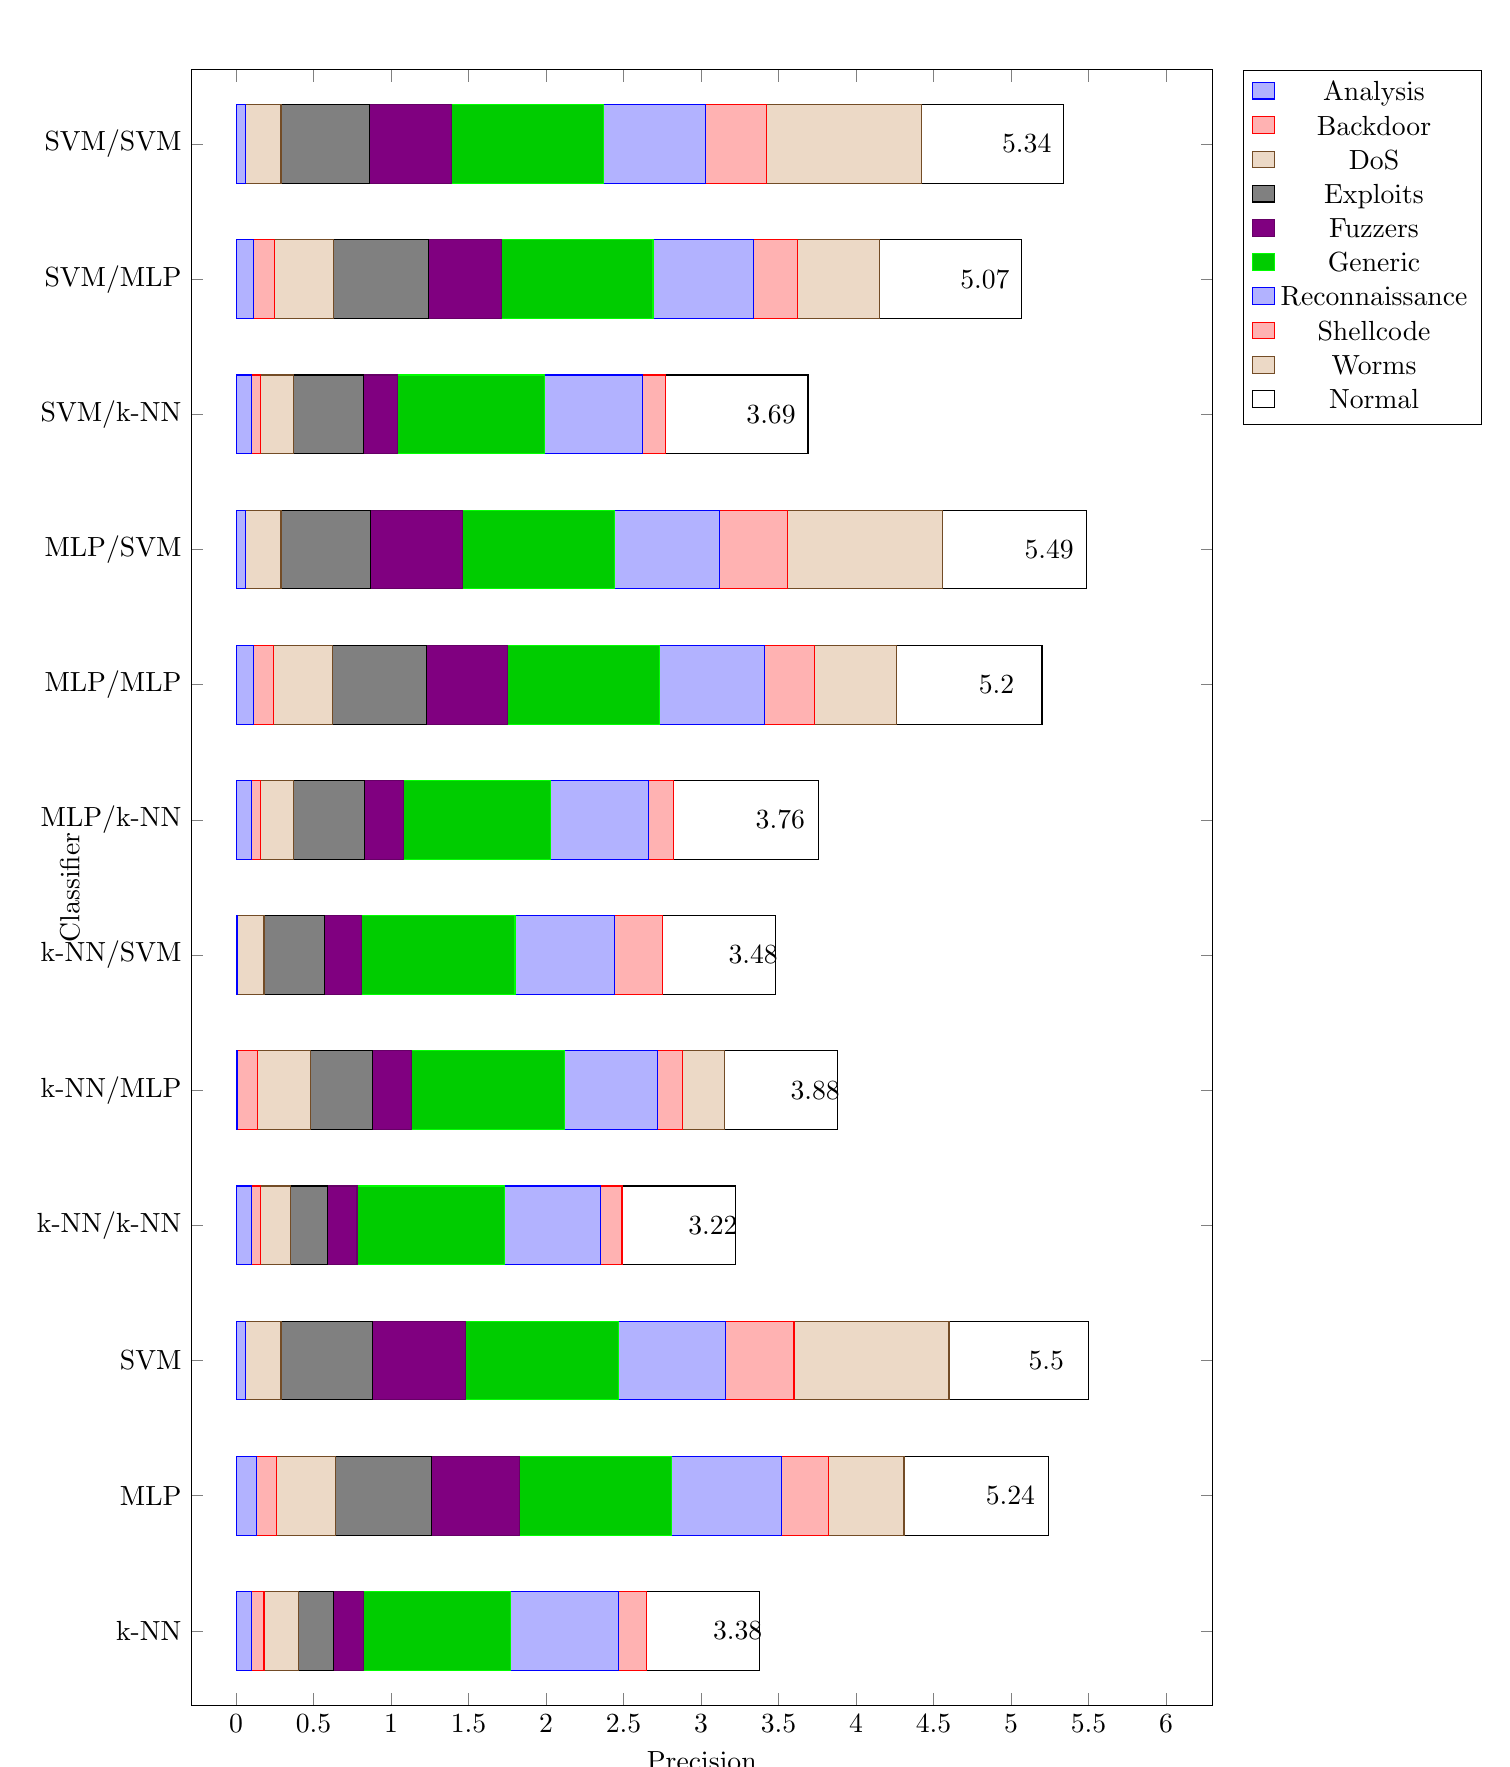
\begin{tikzpicture}
\begin{axis}[
    xbar stacked,
    enlargelimits=0.05,
    legend pos=outer north east,
    ylabel={Classifier},
    xlabel={Precision},
    y label style={at={(axis description cs:-0.1,.5)},anchor=south},
    symbolic y coords={k-NN,MLP,SVM,k-NN/k-NN,k-NN/MLP,k-NN/SVM,MLP/k-NN,MLP/MLP,MLP/SVM,SVM/k-NN,SVM/MLP,SVM/SVM},
    ytick=data,
    %nodes near coords,
    %nodes near coords align={horizontal},
    point meta=rawx,
    bar width = 1cm,
    xmax = 6,
    width=1.2\textwidth,
    height=0.8\paperheight
    ]
    % Analysis
    \addplot coordinates {(0.10,k-NN) (0.13,MLP) (0.06,SVM) 
	                  (0.10,k-NN/k-NN) (0.01,k-NN/MLP) (0.01,k-NN/SVM) 
		          (0.10,MLP/k-NN) (0.11,MLP/MLP) (0.06,MLP/SVM) 
		          (0.10,SVM/k-NN) (0.11,SVM/MLP) (0.06,SVM/SVM)};
    % Backdoor
    \addplot coordinates {(0.08,k-NN) (0.13,MLP) (0.00,SVM) 
	                  (0.06,k-NN/k-NN) (0.13,k-NN/MLP) (0.00,k-NN/SVM) 
		          (0.06,MLP/k-NN) (0.13,MLP/MLP) (0.00,MLP/SVM) 
		          (0.06,SVM/k-NN) (0.14,SVM/MLP) (0.00,SVM/SVM)};
    % DoS
    \addplot  coordinates {(0.22,k-NN) (0.38,MLP) (0.23,SVM) 
	                  (0.19,k-NN/k-NN) (0.34,k-NN/MLP) (0.17,k-NN/SVM) 
		          (0.21,MLP/k-NN) (0.38,MLP/MLP) (0.23,MLP/SVM) 
		          (0.21,SVM/k-NN) (0.38,SVM/MLP) (0.23,SVM/SVM)};
    % Exploits
    \addplot  coordinates {(0.23,k-NN) (0.62,MLP) (0.59,SVM) 
	                  (0.24,k-NN/k-NN) (0.40,k-NN/MLP) (0.39,k-NN/SVM) 
		          (0.46,MLP/k-NN) (0.61,MLP/MLP) (0.58,MLP/SVM) 
		          (0.45,SVM/k-NN) (0.61,SVM/MLP) (0.57,SVM/SVM)};
    % Fuzzers
    \addplot  coordinates {(0.19,k-NN) (0.57,MLP) (0.60,SVM) 
	                  (0.19,k-NN/k-NN) (0.25,k-NN/MLP) (0.24,k-NN/SVM) 
		          (0.25,MLP/k-NN) (0.52,MLP/MLP) (0.59,MLP/SVM) 
		          (0.22,SVM/k-NN) (0.47,SVM/MLP) (0.53,SVM/SVM)};
    % Generic
    \addplot coordinates {(0.95,k-NN) (0.98,MLP) (0.99,SVM) 
	                  (0.95,k-NN/k-NN) (0.99,k-NN/MLP) (0.99,k-NN/SVM) 
		          (0.95,MLP/k-NN) (0.98,MLP/MLP) (0.98,MLP/SVM) 
		          (0.95,SVM/k-NN) (0.98,SVM/MLP) (0.98,SVM/SVM)};
    % Reconnaissance
    \addplot coordinates {(0.70,k-NN) (0.71,MLP) (0.69,SVM) 
	                  (0.62,k-NN/k-NN) (0.60,k-NN/MLP) (0.64,k-NN/SVM) 
		          (0.63,MLP/k-NN) (0.68,MLP/MLP) (0.68,MLP/SVM) 
		          (0.63,SVM/k-NN) (0.65,SVM/MLP) (0.66,SVM/SVM)};
    % Shellcode
    \addplot coordinates {(0.18,k-NN) (0.30,MLP) (0.44,SVM) 
	                  (0.14,k-NN/k-NN) (0.16,k-NN/MLP) (0.31,k-NN/SVM) 
		          (0.16,MLP/k-NN) (0.32,MLP/MLP) (0.44,MLP/SVM) 
		          (0.15,SVM/k-NN) (0.28,SVM/MLP) (0.39,SVM/SVM)};
    % Worms
    \addplot coordinates {(0.00,k-NN) (0.49,MLP) (1.00,SVM) 
	                  (0.00,k-NN/k-NN) (0.27,k-NN/MLP) (0.00,k-NN/SVM) 
		          (0.00,MLP/k-NN) (0.53,MLP/MLP) (1.00,MLP/SVM) 
		          (0.00,SVM/k-NN) (0.53,SVM/MLP) (1.00,SVM/SVM)};
    % Normal
    \addplot [point meta = x, nodes near coords, nodes near coords align={anchor=west}] coordinates {(0.73,k-NN) (0.93,MLP) (0.90,SVM) 
	                  (0.73,k-NN/k-NN) (0.73,k-NN/MLP) (0.73,k-NN/SVM) 
		          (0.94,MLP/k-NN) (0.94,MLP/MLP) (0.93,MLP/SVM) 
		          (0.92,SVM/k-NN) (0.92,SVM/MLP) (0.92,SVM/SVM)};


        \legend{Analysis, Backdoor, DoS, Exploits, Fuzzers, Generic, Reconnaissance, Shellcode, Worms, Normal}
\end{axis}
\end{tikzpicture}
\end{adjustbox}
\caption{Classifiers Precision Graph}
\end{figure}


\newpage


\end{appendices}

\end{document}
